\documentclass[american,]{article}
\usepackage{lmodern}
\usepackage{amssymb,amsmath}
\usepackage{ifxetex,ifluatex}
\usepackage{fixltx2e} % provides \textsubscript
\ifnum 0\ifxetex 1\fi\ifluatex 1\fi=0 % if pdftex
  \usepackage[T1]{fontenc}
  \usepackage[utf8]{inputenc}
\else % if luatex or xelatex
  \ifxetex
    \usepackage{mathspec}
  \else
    \usepackage{fontspec}
  \fi
  \defaultfontfeatures{Ligatures=TeX,Scale=MatchLowercase}
\fi
% use upquote if available, for straight quotes in verbatim environments
\IfFileExists{upquote.sty}{\usepackage{upquote}}{}
% use microtype if available
\IfFileExists{microtype.sty}{%
\usepackage{microtype}
\UseMicrotypeSet[protrusion]{basicmath} % disable protrusion for tt fonts
}{}
\usepackage[margin=1in]{geometry}
\usepackage{hyperref}
\hypersetup{unicode=true,
            pdftitle={Improving Convergence Diagnostics of Iterative Algorithms},
            pdfauthor={Aki Vehtari, Andrew Gelman, Daniel Simpson, Bob Carpenter, Paul Bürkner},
            pdfkeywords={keywords},
            pdfborder={0 0 0},
            breaklinks=true}
\urlstyle{same}  % don't use monospace font for urls
\ifnum 0\ifxetex 1\fi\ifluatex 1\fi=0 % if pdftex
  \usepackage[shorthands=off,main=american]{babel}
\else
  \usepackage{polyglossia}
  \setmainlanguage[variant=american]{english}
\fi
\usepackage{natbib}
\bibliographystyle{plainnat}
\usepackage{placeins}
\usepackage{graphicx,grffile}
\makeatletter
\def\maxwidth{\ifdim\Gin@nat@width>\linewidth\linewidth\else\Gin@nat@width\fi}
\def\maxheight{\ifdim\Gin@nat@height>\textheight\textheight\else\Gin@nat@height\fi}
\makeatother
% Scale images if necessary, so that they will not overflow the page
% margins by default, and it is still possible to overwrite the defaults
% using explicit options in \includegraphics[width, height, ...]{}
\setkeys{Gin}{width=\maxwidth,height=\maxheight,keepaspectratio}
\IfFileExists{parskip.sty}{%
\usepackage{parskip}
}{% else
\setlength{\parindent}{0pt}
\setlength{\parskip}{6pt plus 2pt minus 1pt}
}
\setlength{\emergencystretch}{3em}  % prevent overfull lines
\providecommand{\tightlist}{%
  \setlength{\itemsep}{0pt}\setlength{\parskip}{0pt}}
\setcounter{secnumdepth}{5}
% Redefines (sub)paragraphs to behave more like sections
\ifx\paragraph\undefined\else
\let\oldparagraph\paragraph
\renewcommand{\paragraph}[1]{\oldparagraph{#1}\mbox{}}
\fi
\ifx\subparagraph\undefined\else
\let\oldsubparagraph\subparagraph
\renewcommand{\subparagraph}[1]{\oldsubparagraph{#1}\mbox{}}
\fi

%%% Use protect on footnotes to avoid problems with footnotes in titles
\let\rmarkdownfootnote\footnote%
\def\footnote{\protect\rmarkdownfootnote}

%%% Change title format to be more compact
\usepackage{titling}

% Create subtitle command for use in maketitle
\newcommand{\subtitle}[1]{
  \posttitle{
    \begin{center}\large#1\end{center}
    }
}

\setlength{\droptitle}{-2em}

  \title{Improving Convergence Diagnostics of Iterative Algorithms}
    \pretitle{\vspace{\droptitle}\centering\huge}
  \posttitle{\par}
    \author{Aki Vehtari, Andrew Gelman, Daniel Simpson, Bob Carpenter, Paul Bürkner}
    \preauthor{\centering\large\emph}
  \postauthor{\par}
    \date{}
    \predate{}\postdate{}
  
\usepackage{booktabs}
\usepackage{longtable}
\usepackage{array}
\usepackage{multirow}
\usepackage[table]{xcolor}
\usepackage{wrapfig}
\usepackage{float}
\usepackage{colortbl}
\usepackage{pdflscape}
\usepackage{tabu}
\usepackage{threeparttable}
\usepackage{threeparttablex}
\usepackage[normalem]{ulem}
\usepackage{makecell}

\usepackage{mathtools}
\usepackage[utf8]{inputenc}
\usepackage[T1]{fontenc}
\usepackage{textcomp}
\usepackage{graphicx,pdflscape}
\usepackage{geometry}
\usepackage{amsmath}
\usepackage{float}
\usepackage{supertabular}
\usepackage{booktabs,caption,fixltx2e}
\usepackage{tcolorbox}
\usepackage{paralist}
\usepackage{multicol}
\setcitestyle{round}
\newcommand\numberthis{\addtocounter{equation}{1}\tag{\theequation}}
\DeclareMathOperator*{\dd}{d}
\DeclareMathOperator{\Cauchy}{Cauchy}
\DeclareMathOperator{\N}{N}
\DeclareMathOperator{\Gam}{Gamma}

\begin{document}
\maketitle
\begin{abstract}
Abstract
\end{abstract}

\hypertarget{introduction}{%
\section{Introduction}\label{introduction}}

Iterative simulation, particularly Markov chain Monte Carlo (MCMC), is
increasingly popular in statistics \citep{Brooks+Gelman:1998},
especially in Bayesian applications where the goal is to represent
posterior inference using a sample of posterior draws. Iterative
simulation algorithms in common use typically can be proven to converge
to the target distribution as the number of draws approaches infinity,
but convergence is only approximate for any finite number of draws.

In practice we have two concerns:

\begin{enumerate}
\item The $M$ chains may not have not mixed well, so that the simulations do not
represent the target distribution because they still retain the influence of
their history.
\item The effective sample size (number of effective simulation draws) is low,
possibly much less than the total number of draws across chains, because
of dependence (autocorrelation) within each chain.
\end{enumerate}

These two issues are related. It is only possible to have a large number
of effective draws if the chains have mixed well. Figure
\ref{converge.challenge} illustrates two ways in which sequences of
iterative simulations can fail to mix. In the first example, two chains
are in different parts of the target distribution, in the second
example, the chains move but have not attained stationarity. This
situation may arise due to multimodal posteriors or because one chain is
stuck in a region of high curvature with a step size too high to make an
acceptable proposal. These two examples make it clear that any method
for assessing mixing and effective sample size should use information
between and within chains.

\begin{figure}
\vspace{-.22\textwidth}
\centerline{\hspace{-.1\textwidth}
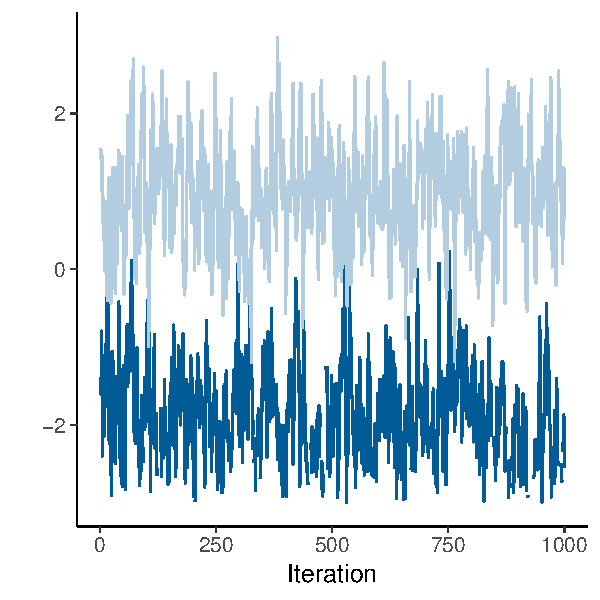
\includegraphics[width=\textwidth]{graphics/convergechallenge1.pdf}
\hspace{-.5\textwidth}
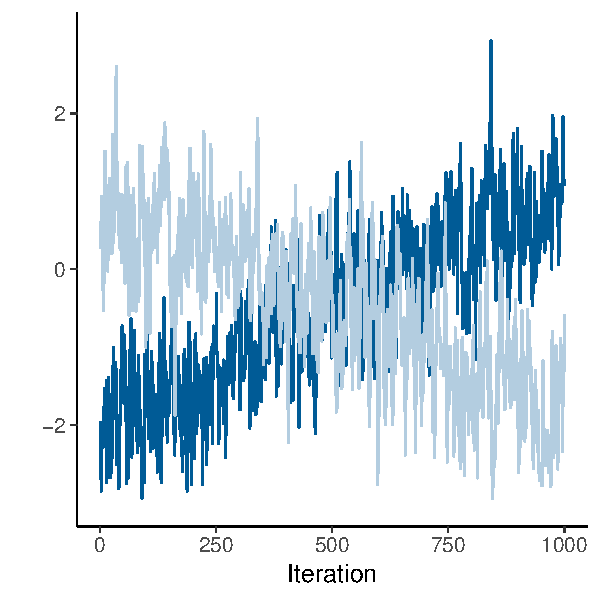
\includegraphics[width=\textwidth]{graphics/convergechallenge2.pdf}}
\vspace{-.22\textwidth}
\caption{\em Examples of two challenges in assessing convergence of iterative
simulations. (a) In the left plot, either sequence alone looks stable, but the
juxtaposition makes it clear that they have not converged to a common
distribution. (b) In the right plot, the two sequences happen to cover a common
distribution but neither sequence appears stationary. These graphs demonstrate
the need to use between-sequence and also within-sequence information when
assessing convergence. From Gelman et al. (2013).}
\label{converge.challenge}
\end{figure}

The other relevant point is that we are often fitting models with large
numbers of parameters, so that it is not realistic to expect to make
trace plots such as in Figure \ref{converge.challenge} for all
quantities of interest. We need numerical summaries that can flag
potential problems. However, as we will show in this paper, the
currently existing and widely applied convergence diagnostics have
serious flaws under some conditions. We will thus propose improvements
to these diagnostics.

\hypertarget{CD}{%
\section{Convergence diagnostics for iterative algorithms}\label{CD}}

The Split-\(\widehat{R}\) statistic and the \emph{effective sample size}
(ESS) are routinely used to monitor the convergence of iterative
simulations, which are omnipresent in Bayesian statistics in the form of
Markov-Chain Monte-Carlo samples. The original \(\widehat{R}\) statistic
\citep{Gelman+Rubin:1992, Brooks+Gelman:1998} and
\emph{split}-\(\widehat{R}\) \citep{BDA3} are both based on the ratio of
between and within-chain marginal variances of the simulations, while
the latter is computed from split chains (hence the name).

\hypertarget{SplitRhat}{%
\subsection{\texorpdfstring{\emph{Split}-\(\widehat{R}\)}{Split-\textbackslash{}widehat\{R\}}}\label{SplitRhat}}

Below, we present the computation of \emph{Split}-\(\widehat{R}\)
following \citet{BDA3}, but using the notation style of
\citet{StanBook}. These implementations represent the current de facto
standard of convergence diagnostics for iterative simulations. In the
equations below, \(N\) is the number of draws per chain, \(M\) is the
number of chains, and \(S=MN\) is the total number of draws from all
chains. For each scalar summary of interest \(\theta\), we compute \(B\)
and \(W\), the between- and within-chain variances:

\begin{align}
B &= \frac{N}{M-1}\sum_{m=1}^{M}(\overline{\theta}^{(.m)} - 
\overline{\theta}^{(..)})^2, \quad \mbox{where} \quad 
\overline{\theta}^{(.m)}=\frac{1}{N}\sum_{n=1}^N \theta^{(nm)}, \quad
\overline{\theta}^{(..)} = \frac{1}{M}\sum_{m=1}^M\overline{\theta}^{(.m)} 
\\
W &= \frac{1}{M}\sum_{m=1}^{M}s_j^2, \quad \mbox{where} \quad
s_m^2=\frac{1}{N-1} \sum_{n=1}^N (\theta^{(nm)}-\overline{\theta}^{(.m)})^2.
\end{align}

The between-chain variance, \(B\), also contains the factor \(N\)
because it is based on the variance of the within-chain means,
\(\overline{\theta}^{(.m)}\), each of which is an average of \(N\)
values \(\theta^{(nm)}\). We can estimate \(\mbox{var}(\theta \mid y)\),
the marginal posterior variance of the estimand, by a weighted average
of \(W\) and \(B\), namely

\begin{equation}
\widehat{\mbox{var}}^+(\theta \mid y) = \frac{N-1}{N}W + \frac{1}{N}B.
\end{equation}

This quantity \emph{overestimates} the marginal posterior variance
assuming the starting distribution of the simulations is appropriately
overdispersed compared to the target distribution, but is
\emph{unbiased} under stationarity (that is, if the starting
distribution equals the target distribution), or in the limit
\(N\rightarrow\infty\). To have an overdispersed starting distribution,
independent Markov chains should be initialized with diffuse starting
values for the parameters.

Meanwhile, for any finite \(N\), the within-chain variance \(W\) should
\emph{underestimate} \(\mbox{var}(\theta \mid y)\) because the
individual chains haven't had the time to explore all of the target
distribution and, as a result, will have less variability. In the limit
as \(N\rightarrow\infty\), the expectation of \(W\) also approaches
\(\mbox{var}(\theta \mid y)\).

We monitor convergence of the iterative simulations to the target
distribution by estimating the factor by which the scale of the current
distribution for \(\theta\) might be reduced if the simulations were
continued in the limit \(N\rightarrow\infty\). This potential scale
reduction is estimated as

\begin{equation}
\widehat{R} = \sqrt{\frac{\widehat{\mbox{var}}^+(\theta \mid y)}{W}},
\end{equation}

which declines to 1 as \(N\rightarrow\infty\). We call this
\emph{split}-\(\widehat{R}\) because we are applying it to chains that
have been split in half so that \(M\) is twice the number of actual
chains. Without splitting, \(\widehat{R}\) would get fooled by
non-stationary chains (see section/appendix).

We note that \emph{split}-\(\widehat{R}\) is also well defined for
sequences that are not Markov-chains. However, for simplicity, we always
refer to `chains' instead of more generally to `sequences' as the former
is our primary use case for \(\widehat{R}\)-like measures.

\hypertarget{ESS}{%
\subsection{Effective sample size}\label{ESS}}

If the \(N\) simulation draws within each chain were truly independent,
the between-chain variance \(B\) would be an unbiased estimate of the
posterior variance, \(\mbox{var}(\theta \mid y)\), and we would have a
total of \(S = MN\) independent simulations from the \(M\) chains. In
general, however, the simulations of \(\theta\) within each chain will
be autocorrelated, and thus \(B\) will be larger than
\(\mbox{var}(\theta \mid y)\), in expectation.

One way to define effective sample size for correlated simulation draws
is to consider the statistical efficiency of the average of the
simulations \(\bar{\theta}^{(..)}\) as an estimate of the posterior mean
\(\mbox{E}(\theta \mid y)\). This also generalizes to posterior
expectations of functionals of parameters \(\mbox{E}(g(\theta) \mid y)\)
and we return later to how to estimate the effective sample size of
quantiles which cannot be presented as expectations. For simplification,
in this section we consider the effective sample size for the posterior
mean.

The effective sample size of a chain is defined in terms of the
autocorrelations within the chain at different lags. The autocorrelation
\(\rho_t\) at lag \(t \geq 0\) for a chain with joint probability
function \(p(\theta)\) with mean \(\mu\) and variance \(\sigma^2\) is
defined to be

\begin{equation}
\rho_t = \frac{1}{\sigma^2} \, \int_{\Theta} (\theta^{(n)} - \mu)
(\theta^{(n+t)} - \mu) \, p(\theta) \, d \theta.
\end{equation}

This is just the correlation between the two chains offset by \(t\)
positions. Because we know \(\theta^{(n)}\) and \(\theta^{(n+t)}\) have
the same marginal distribution in an MCMC setting, multiplying the two
difference terms and reducing yields

\begin{equation}
\rho_t = \frac{1}{\sigma^2} \, \int_{\Theta} \theta^{(n)} \, \theta^{(n+t)}
\, p(\theta) \, d \theta.
\end{equation}

The effective sample size of one chain generated by a process with
autocorrelations \(\rho_t\) is defined by

\begin{equation}
N_{\rm eff} \ = \
\frac{N}{\sum_{t = -\infty}^{\infty} \rho_t} \ = \
\frac{N}{1 + 2 \sum_{t = 1}^{\infty} \rho_t}.
\end{equation}

Effective sample size \(N_{\rm eff}\) can be larger than \(N\) in case
of antithetic Markov chains, which have negative autocorrelations on odd
lags. The Dynamic Hamiltonian Monte-Carlo algorithms used in Stan
\citep{Hoffman+Gelman:2014, betancourt2017conceptual} can produce
\(N_{\rm eff}>N\) for parameters with a close to Gaussian posterior (in
the unconstrained space) and low dependency on other parameters.

In practice, the probability function in question cannot be tractably
integrated and thus neither autocorrelation nor the effective sample
size can be calculated. Instead, these quantities must be estimated from
the samples themselves. The rest of this section describes an
autocorrelation and split-\(\widehat{R}\) based effective sample size
estimator, based on multiple split chains. For simplicity, each chain
will be assumed to be of the same length \(N\).

Computations of autocorrelations for all lags simultaneously can be done
via the fast Fourier transform algorithm \citep[FFT; see][ for more
details]{Geyer:2011}. The autocorrelation estimates \(\hat{\rho}_{t,m}\)
at lag \(t\) from multiple chains \(m \in (1,\ldots,M)\) are combined
with the within-chain variance estimate \(W\) and the multi-chain
variance estimate \(\widehat{\mbox{var}}^{+}\) introduced above to
compute the combined autocorrelation at lag \(t\) as

\begin{equation}
\hat{\rho}_t
= 1 - \frac{\displaystyle W - \textstyle \frac{1}{M}\sum_{m=1}^M 
\hat{\rho}_{t,j}}{\widehat{\mbox{var}}^{+}}. \label{rhohat}
\end{equation}

If the chains have not converged, the variance estimator
\(\widehat{\mbox{var}}^{+}\) will overestimate the true marginal
variance which leads to an overestimation of the autocorrelation and an
underestimation of the effective sample size.

Because of noise in the correlation estimates \(\hat{\rho}_t\) increases
as \(t\) increases, typically the truncated sum of \(\hat{\rho}_t\) is
used. Negative autocorrelations can happen only on odd lags and by
summing over pairs starting from lag \(t=0\), the paired autocorrelation
is guaranteed to be positive, monotone and convex modulo estimator noise
\citep{Geyer:1992, Geyer:2011}. The effective sample size of combined
chains is then defined as

\begin{equation}
S_{\rm eff} = \frac{N \, M}{\hat{\tau}},
\end{equation} where \begin{equation}
\hat{\tau} = 1 + 2 \sum_{t=1}^{2k+1} \hat{\rho}_t = 
-1 + 2 \sum_{t'=0}^{k} \hat{P}_{t'},
\end{equation}

and \(\hat{P}_{t'}=\hat{\rho}_{2t'}+\hat{\rho}_{2t'+1}\). The initial
positive sequence estimator is obtained by choosing the largest \(k\)
such that \(\hat{P}_{t'}>0\) for all \(t' = 1,\ldots,k\). The initial
monotone sequence estimator is obtained by further reducing
\(\hat{P}_{t'}\) to the minimum of the preceding values so that the
estimated sequence becomes monotone.

The effective sample size \(S_{\rm eff}\) described here is different
from similar formulas in the literature in that we use multiple chains
and between-chain variance in the computation, which typically gives us
more conservative claims (lower values of \(S_{\rm eff}\)) compared to
single chain estimates, especially when mixing of the chains is poor. If
the chains are not mixing at all (e.g., the posterior is multimodal and
the chains are stuck in different modes), then our \(S_{\rm eff}\) is
close to the number of chains.

\hypertarget{problems-of-current-diagnostics}{%
\subsection{Problems of current
diagnostics}\label{problems-of-current-diagnostics}}

\emph{split}-\(\widehat{R}\), and \(S_{\rm eff}\) are well defined
only if the marginal posteriors have finite mean and variance, which is not always the case. \emph{split}-\(\widehat{R}\), and \(S_{\rm eff}\) can also be unstable even if the mean and variance are finite, if the marginal distribution has thick tails. Usually \emph{split}-\(\widehat{R}\), and \(S_{\rm eff}\) are computed only for the posterior mean, which can miss convergence and sampling efficiency problems in tails which affect, for example, the posterior interval estimates.

\hypertarget{improving-convergence-diagnostics}{%
\section{Improving convergence
diagnostics}\label{improving-convergence-diagnostics}}

In this section, we discuss several measures that, together, can solve
the problems of the current divergence diagnostics we identified above.

\hypertarget{rank-normalization}{%
\subsection{Rank normalization}\label{rank-normalization}}

As \emph{split}-\(\widehat{R}\), and \(S_{\rm eff}\) are well defined
only if the marginal posteriors have finite mean and variance, we
propose to use rank normalized parameter values instead of the actual
parameter values for the purpose of diagnosing convergence.

Rank normalized \emph{split}-\(\widehat{R}\) and \(S_{\rm eff}\) are
computed using the equations in Section \ref{CD}, but
replacing the original parameter values \(\theta^{(nm)}\) with their
corresponding rank normalized values denoted as \(z^{(nm)}\). Rank
normalization is done a follows: First, replace each value
\(\theta^{(nm)}\) by its rank \(r^{(nm)}\). Average rank for ties are
used to conserve the number of unique values of discrete quantities.
Ranks are computed jointly for all draws from all chains. Second,
normalize ranks via the inverse normal transformation
\begin{equation}
z^{(nm)} = \phi^{-1}((r^{(nm)}-1/2)/S).
\end{equation}
See online appendix for illustration of rank normalization.

For continuous variables and \(S \rightarrow \infty\), the rank
normalized values are normally distributed. Using normalized ranks
\(z^{(nm)}\) instead of ranks \(r^{(nm)}\) themselves has the additional
benefit that the behavior of \(\widehat{R}\) and \(S_{\rm eff}\) do
not change for normally distributed parameters.

We will use the term \emph{bulk effective sample size} (bulk-ESS or
bulk-\(S_{\rm eff}\)) to refer to the effective sample size based on the
rank normalized draws. Bulk-ESS is useful for diagnosing problems due to
trends or different locations of the chains (see section/appendix). Further, it is
well defined even for distributions with infinite mean or variance, a
case where previous ESS estimates fail. However, due to the rank
normalization, Bulk-ESS is no longer directly applicable to estimate the
Monte Carlo standard error of the posterior mean. We will come back to
the issue of computing Monte Carlo standard errors for relevant
quantities in Section \ref{mcse}.

\hypertarget{diagnostics-for-folded-draws}{%
\subsection{Diagnostics for folded
draws}\label{diagnostics-for-folded-draws}}

Both original and rank-normalized \emph{split}-\(\widehat{R}\) can be
fooled if the chains have different scales but the same location as
shown in (see section/appendix). To alleviate this problem, we propose to compute a
rank normalized \emph{split}-\(\widehat{R}\) statistic not only for the
original draws \(\theta^{(nm)}\), but also for the corresponding folded
draws \(\zeta^{(mn)}\), that is the absolute deviations from the median
\begin{equation}
\label{zeta}
\zeta^{(mn)} = {\rm abs}(\theta^{(nm)}-{\rm median}(\theta)).
\end{equation}

The rank-normalized \emph{split}-\(\widehat{R}\) measure computed on the
basis of \(\zeta^{(mn)}\) will be called rank-normalized
\emph{folded-split}-\(\widehat{R}\). It measures convergence in the
tails rather than in the bulk of the distribution. To obtain a single
conservative \(\widehat{R}\) estimate, we propose to report the maximum
of rank normalized \emph{split}-\(\widehat{R}\) and rank normalized
\emph{folded-split}-\(\widehat{R}\) for each parameter.

\hypertarget{convergence-diagnostics-for-quantiles}{%
\subsection{Convergence diagnostics for
quantiles}\label{convergence-diagnostics-for-quantiles}}

The new \(\widehat{R}\) and bulk-ESS introduced above are useful as overall efficiency
measures. Next we introduce
convergence diagnostics for quantiles and related quantities, which are more focused measures and help to diagnose reliability of often reported
posterior intervals. Estimating
the efficiency of quantile estimates has a high practical
relevance in particular as we observe the efficiency for tail quantiles
to often be lower than for the mean or median.

The \(\alpha\)-quantile
is defined as the parameter value \(\theta_\alpha\) for which
\(p(\theta \leq \theta_\alpha) = \alpha\). An estimate
\(\hat{\theta}_\alpha\) of \(\theta_\alpha\) can thus be obtained by
finding the \(\alpha\)-quantile of the empirical CDF (ECDF) of the
posterior draws \(\theta^{(s)}\). However, quantiles cannot be written
as an expectation, and thus the above equations for \(\widehat{R}\) and
\(S_{\rm eff}\) are not directly applicable. Thus, we first focus on the
efficiency estimate for the cumulative probability
\(p(\theta \leq \theta_\alpha)\) for different values of
\(\theta_\alpha\).

For any \(\theta_\alpha\), the ECDF gives an estimate of the cumulative
probability
\begin{equation}
p(\theta \leq \theta_\alpha) \approx \bar{I}_\alpha = \frac{1}{S}\sum_{s=1}^S
I(\theta^{(s)} \leq\theta_\alpha),
\end{equation}
where \(I()\) is the indicator function. The indicator function
transforms simulation draws to 0's and 1's, and thus the subsequent
computations are bijectively invariant. Efficiency estimates of the ECDF
at any \(\theta_\alpha\) can now be obtained by applying
rank-normalizing and subsequent computations directly on the indicator
function's results.

Assuming that we know the CDF to be a certain continuous function \(F\)
which is smooth near an \(\alpha\)-quantile of interest, we could use
the delta method to compute a variance estimate for
\(F^{-1}(\bar{I}_\alpha)\). Although we don't usually know \(F\), the
delta method approach reveals that the variance of \(\bar{I}_\alpha\)
for some \(\theta_\alpha\) is scaled by the (usually unknown) density
\(f(\theta_\alpha)\), but the efficiency depends only on the efficiency
of \(\bar{I}_\alpha\). Thus, we can use the effective sample size for
the ECDF (we computed using the indicator function
\(I(\theta^{(s)} \leq \theta_\alpha)\)) also for the corresponding
quantile estimates.
%
See online appendix for more details variance of the cumulative
distribution function.

To get a better sense of the efficiency of the chains in the
distributions' tails, we propose to compute the minimum of the effective
sample sizes of the 5\% and 95\% quantiles, which we will call
\emph{tail effective sample size} (tail-ESS or tail-\(S_{\rm eff}\)).
Tail-ESS can help diagnosing problems due to different scales of the
chains (see section/appendix).

% TODO: I (Paul) think we need to justify shortly why we compute ``tail-Rhat''
% (i.e., \emph{folded-split}-\(\widehat{R}\)) based on the folded draws,
% but tail-ESS based on tail quantiles.

\hypertarget{efficiency-estimates-for-the-median-absolute-deviation}{%
\subsection{Efficiency estimates for the median absolute
deviation}\label{efficiency-estimates-for-the-median-absolute-deviation}}

Since the marginal posterior distributions might not have finite mean
and variance, by default RStan \citep{RStan.2.17} and RStanARM
\citep{RStanARM.2.17} report median and median absolute deviation (MAD)
instead of mean and standard error (SE). Median and MAD are well defined
even when the marginal distribution does not have finite mean and
variance. Since the median is just 50\%-quantile, we can get an
efficiency estimate for it as for any other quantile.

Further, we can also compute an efficiency estimate for the median
absolute deviation (MAD) by computing the efficiency estimate of an
indicator function based on the folded parameter values \(\zeta\) (see
Equation (\ref{zeta})):
\begin{equation}
p(\zeta \leq \zeta_{0.5}) \approx \bar{I}_{\zeta,0.5} = \frac{1}{S}\sum_{s=1}^S
I(\zeta^{(s)} \leq \zeta_{0.5}),
\end{equation}
where \(\zeta_{0.5}\) is the median of the folded values. We see that
the efficiency estimate for the MAD is obtained by applying the same
approach as for the median (and other quantiles) but with the folded
parameters values also used in the computation of the tail-ESS.

\hypertarget{small_interval_S_eff}{%
\subsection{Efficiency estimates for small interval probability
estimates}\label{small_interval_S_eff}}

We can get more local efficiency estimates by considering small
probability intervals. We propose to compute the efficiency estimates
for
\begin{equation}
\bar{I}_{\alpha,\delta} = p(\hat{Q}_\alpha < \theta \leq \hat{Q}_{\alpha+\delta}),
\end{equation}

where \(\hat{Q}_\alpha\) is an empirical \(\alpha\)-quantile,
\(\delta=1/k\) is the length of the interval with some positive integer
\(k\), and \(\alpha \in (0,\delta,\ldots,1-\delta)\) changes in steps of
\(\delta\). Each interval has \(S/k\) draws, and the efficiency measures
the autocorrelation of an indicator function which is \(1\) when the
values are inside the specific interval and \(0\) otherwise. This gives
us a local efficiency measure which does not depend on the shape of the
distribution.

\hypertarget{mcse}{%
\subsection{Monte Carlo error estimates for quantiles}\label{mcse}}

It is common practice to only report the Monte Carlo error of the mean,
but not of quantiles and related quantities. As the delta method for
computing the variance would require explicit knowledge of the
normalized posterior density, which we don't have in most non-trivial
cases, we propose the following alternative approach to compute Montor
Carlo standard errors of quantiles:

\begin{enumerate}
\def\labelenumi{\arabic{enumi}.}
\item
  Compute quantiles of the Beta distribution with shape parameters
  \begin{equation}
  \beta_1 = S_{\rm eff} / S \times \bar{I}_\alpha+1 \quad \text{and} \quad
  \beta_2 = S_{\rm eff} / S \times (1-\bar{I}_\alpha) + 1.
  \end{equation} Including \(S_{\rm eff}/S\) takes into account the
  efficiency of the posterior draws.
\item
  Find indices in \(s \in \{1,\ldots,S\}\) closest to the ranks of these
  quantiles. For example, for quantile \(Q\), find
  \(s = {\rm round(Q \times S)}\).
\item
  Use the corresponding \(\theta^{(s)}\) from the list of sorted
  posterior draws as quantiles from the error distribution. These
  quantiles can be used to approximate the Monte Carlo standard error.
\end{enumerate}

\hypertarget{warning-thresholds}{%
\subsection{Interpreting \texorpdfstring{\emph{Split}-\(\widehat{R}\)}{Split-\textbackslash{}widehat\{R\}}, ESS, and MCSE}\label{warning-thresholds}}

The ultimate focus should be in the accuracy of the estimate for the
quantity of interest. This accuracy can be measure using Monte Carlo
standard error (or corresponding interval) and the acceptable MCSE
depends on the quantity and application. MCSE estimate is computed
using the marginal posterior of the quantity and adjusted using ESS,
and ESS is based on \emph{split}-\(\widehat{R}\) and autocorrelations
of the chains.

In cases of easy sampling, we could compute ESS only based on the
autocorrelations, but \emph{split}-\(\widehat{R}\) is very helpful in
case of multimodality or other reasons causing chains to get stuck in
part of the target distribution (e.g. in case of unimodal funnel and
HMC, differences in step size adaptation can lead to chains to have
different behavior reaching the narrow part of the funnel). In case of
well separated multimodality the \emph{split}-\(\widehat{R}\)
adjustment of ESS, makes the ESS estimate to be close to the number of
distinct modes. If only one chain would be run, and ESS would be
computed only based on autocorrelations, the ESS would be highly
over-estimated. The variance of \emph{split}-\(\widehat{R}\) adjusted
ESS could be improved by running more chains. We recommend running at
least four chains. The \emph{split}-\(\widehat{R}\) is not alone
directly determining the MCSE, as it only inflates ESS estimate which
is part of MCSE computation. As a generic ad hoc rule based on the
simulations we recommend to aim for \emph{split}-\(\widehat{R}<1.01\).

The required ESS can be ultimately decided only in the context of MCSE
of the quantity of interest. However, there are two reasons to look at
the ESS before MCSEs. Firstly, the computation of
\emph{split}-\(\widehat{R}\) and autocorrelations needed for ESS
itself require estimating means and variances, and in order to get
reliable convergence and ESS estimate, we recommend to aim for
ESS$>400$. In case of running four chains, this corresponds to having
at least effective sample size of 50 per each split chain to be used
for estimating means, variances and autocorrelations. Often for a
useful estimation accuracy ESS$>100$ would be sufficient, but that
would require that we know that ESS$>100$, and when we don't know that
we need higher ESS to be certain about the sampling efficiency.
Secondly, effective sample sizes for different parameters are on the
same scale, and thus it is easier to see which part of the model might
have sampling problems.

After checking that \emph{split}-\(\widehat{R}\) and ESS fullfil the
above ad hoc requirements, we recommend to take int account the
application specific requirements for the accuracy of the quantity of
interest and check that MCSE is low enough or continue sampling.

% Based on the experiments presented in
% \protect\hyperlink{AppendixD}{Appendices D-F}, more strict convergence
% diagnostics and effective sample size warning limits could be used. We
% propose the following warning thresholds although additional
% experiments would be useful:

% \begin{itemize}
% \tightlist
% \item
%   Rhat \textgreater{} 1.01
% \item
%   ESS \textless{} 400
% \end{itemize}

% In case of running 4 chains, an effective sample size of 400 corresponds
% to having an effective sample size of 50 for each 8 split chains, which
% we consider to be minimum for reliable mean, variance and
% autocorrelation estimates needed for the convergence diagnostic. We
% recommend running at least 4 chains to get reliable between chain
% variances for the convergence diagnostics.

% Plots shown in the upcoming sections have dashed lines based on these
% thresholds (in continuous plots, a dashed line at 1.005 is plotted
% instead of 1.01, as values larger than that are usually rounded in our
% summaries to 1.01).

\hypertarget{diagnostic-visualizations}{%
\subsection{Diagnostic visualizations}\label{diagnostic-visualizations}}

In order to intuitively grasp convergence of iterative algorithms, we
propose several new diagnostic visualizations in addition to the numeric
convergence diagnostics discussed above. We will illustrate the usage of
these visualizations by means of several examples in Section
\ref{examples}.

\hypertarget{rank-plots}{%
\subsubsection{Rank plots}\label{rank-plots}}

Extending the idea of using ranks instead of the original parameter
values, we propose to use rank plots for each chain instead
of trace plots. Rank plots are nothing else than histograms of the
ranked posterior samples (ranked over all chains) plotted separately for
each chain. If rank plots of all chains look similar, this indicates
good mixing of the chains. As compared to trace plots, rank plots don't
tend to squeeze to a fuzzy mess in case of long chains.

\hypertarget{quantile-and-small-interval-plots}{%
\subsubsection{Quantile and small interval
plots}\label{quantile-and-small-interval-plots}}

The efficiency of quantiles or small interval probabilities may vary
drastistically across different quantiles and small interval positions,
respectively. We thus propose to use diagnostic plots that display
efficiency of quanilites or small interval probabilities across their
whole range to better diagnose areas of the distributions that the
iterative algorithm fails to explore efficiently.

\hypertarget{efficiency-change-plots}{%
\subsubsection{Efficiency per iteration plots}\label{efficiency-change-plots}}

For a well explored distribution, we expect the ESS measures to grow
linearly with the total number of draws \(S\), or, equivalently, that
the relative efficiency (ESS divided \(S\)) is approximately constant
for different values of \(S\). For small number of draws, both bulk and
tail-ESS may be unreliable and cannot necessarily detect convergence
problems (see section/appendix). As a result, some convergence problems may only be
detectable as \(S\) increases, which then implies the ESS to grow slower
then linear or even decrease with increasing \(S\). Equivalently, in
such a case, we would expect to see a relatively sharp drop in the
relative efficiency measures. We therefore propose to plot the change of
both bulk and tail ESS with increasing \(S\). This can be done based on
a single model without a need to refit, as we can just extract initial
sequences of certain length from the original chains. However, it should
be noted that some convergence problems only occur at relatively high
\(S\) and may thus not be detectable if the total number of draws is too
small.

\hypertarget{examples}{%
\section{Examples}\label{examples}}

In this section, we will go through some examples to demonstrate the
usefulness of our proposed methods as well as the associated workflow
in determining convergence. The online appendix contains all model
details, code to reproduce the results and more detailed analysis of
different algorithm variants and further
examples\footnote{\url{https://avehtari.github.io/rhat_ess/rhat_ess.html}}.

We use either dynamic Hamiltonian Monte Carlo with multinomial
sampling \citep{betancourt2017conceptual} as implemented in Stan
\citep{StanManual.2.18.0} or Gibbs sampling as implemented in JAGS.

\hypertarget{cauchy-a-distribution-with-infinite-mean-and-variance}{%
\subsection{Cauchy: A distribution with infinite mean and
variance}\label{cauchy-a-distribution-with-infinite-mean-and-variance}}

The classic \emph{split}-\(\widehat{R}\) are based on calculating
within and between chain variances. If the marginal distribution of a
chain is such that the variance is not defined (i.e., infinite), the
classic \emph{split}-\(\widehat{R}\) is not well justified. In this
section, we will use the Cauchy distribution as an example of such a
distribution. 

\hypertarget{nominal-parameterization-of-cauchy}{%
\subsubsection{Nominal parameterization of
Cauchy}\label{nominal-parameterization-of-cauchy}}

% \begin{verbatim}
% parameters {
%   vector[50] x;
% }

% model {
%   x ~ cauchy(0, 1);
% }

% generated quantities {
%   real I = fabs(x[1]) < 1 ? 1 : 0;
% }
% \end{verbatim}

% \hypertarget{default-stan-options}{%
% \paragraph{Default Stan options}\label{default-stan-options}}

% Run the nominal model:

The nominal Cauchy model with direct parameterization is
\begin{align}
  x \sim \Cauchy(0,1).
\end{align}
We set independent Cauchy distribution for 50 dimensional vector $x$.
We use dynamic HMC and run 4 chains each with 1000 iterations of
warmup and 1000 iterations stored. Dynamic HMC specific diagnostics
treedepth exceedences and Bayesian fraction of missing information
indicate slow mixing of the chains.

% \begin{verbatim}
% Inference for the input samples (4 chains: each with iter = 2000; warmup = 1000):

%           Q5    Q50    Q95   Mean     SD  Rhat Bulk_ESS Tail_ESS
% x[1]   -5.74  -0.01   6.31   2.50  36.40  1.03     1181      393
% x[2]   -5.83  -0.01   6.07   0.65  16.20  1.01     2645      502
% x[3]   -5.23   0.01   5.73   0.58  17.70  1.01     2683      823
% x[4]   -6.25  -0.02   6.90   0.16  11.50  1.01     3627      644
% x[5]   -9.66  -0.05   5.11  -1.41  11.30  1.01      629      156
% x[6]   -5.26   0.00   5.41   0.20   5.32  1.01     3060      883
% x[7]   -6.35   0.06  10.80   4.14  32.60  1.02      607      184
% x[8]   -6.45  -0.01   5.37  -0.22   7.66  1.00     2658      886
% x[9]   -6.53   0.00   6.30   0.15   7.38  1.01     3128      901
% x[10]  -6.12  -0.01   5.92   0.06   5.74  1.01     2421      642
% x[11]  -6.73   0.00   6.15   0.03   9.68  1.01     2079      600
% x[12]  -5.68  -0.03   4.88   0.19  17.50  1.00     2633      774
% x[13]  -4.53  -0.06   4.27   0.09   6.28  1.00     3148      811
% x[14]  -4.88   0.00   5.03  -0.02   5.93  1.00     1461      492
% x[15] -14.50  -0.01  11.50  -1.41  22.70  1.03      486      160
% x[16]  -7.03   0.01   6.96   0.16  15.90  1.01     2329      463
% x[17]  -6.59   0.01   7.69   0.96  30.20  1.01     2292      446
% x[18]  -4.51   0.05   6.92   1.10  11.90  1.01     2640      447
% x[19]  -7.66  -0.05   6.08  -3.14  28.10  1.01     1147      298
% x[20]  -5.78   0.03  11.30   5.78  37.00  1.03      363       80
% x[21]  -4.89   0.02   5.38   0.11   5.45  1.01     3276      824
% x[22]  -5.59   0.04   5.37   0.49  15.40  1.01     2121      522
% x[23] -14.40   0.01   7.00  -3.10  32.00  1.01      391       89
% x[24]  -5.93  -0.04   5.47  -1.01  16.60  1.02     1434      284
% x[25]  -7.07  -0.02   5.94  -1.76  21.30  1.01     1544      324
% x[26]  -8.96  -0.06   5.85  -1.97  17.40  1.01     1778      452
% x[27]  -8.81  -0.01   8.34   0.15  18.10  1.00     1816      352
% x[28]  -5.26   0.02   5.93   0.11   9.51  1.02     3776      675
% x[29]  -5.88   0.00   5.90  -0.04  18.50  1.01     3642      846
% x[30]  -5.57  -0.02   5.14  -0.18   6.22  1.00     4363      643
% x[31]  -7.36   0.01   7.25   0.07   8.71  1.00     3384      896
% x[32]  -8.85  -0.04   6.50 -10.20  81.20  1.01      561      141
% x[33]  -4.79   0.03   4.96  -0.35   8.61  1.01     2626      735
% x[34]  -5.91  -0.03   5.37  -0.11   5.96  1.01     2408      634
% x[35]  -6.10   0.02   6.79  -0.33  14.60  1.01     2654      630
% x[36]  -4.86   0.10  15.60  19.30 108.00  1.04      155       34
% x[37]  -8.93   0.00   7.86  -0.09  13.30  1.01     1155      427
% x[38]  -5.54  -0.02   4.83  -0.33   5.95  1.00     3353      576
% x[39]  -5.89  -0.03   5.84   0.11   7.29  1.02     4493      724
% x[40]  -8.71   0.01   6.71  -1.98  19.80  1.00      877      148
% x[41]  -6.88  -0.03   7.55  -0.27  11.30  1.00     1726      512
% x[42]  -6.15   0.01   6.48   0.09  15.50  1.01     1519      448
% x[43]  -6.38   0.00   7.39   0.11  12.10  1.01     2746      483
% x[44]  -7.84   0.00   7.99   0.41  11.50  1.01     2999      659
% x[45]  -4.77  -0.02   4.66   0.04   6.73  1.01     2904     1014
% x[46]  -4.84   0.00   5.99   1.16  22.10  1.00      955      338
% x[47]  -8.51   0.03  24.30   0.80  37.10  1.07      231       56
% x[48]  -6.73   0.00   5.33  -0.72  10.40  1.01     1907      469
% x[49]  -6.27   0.04   6.92   0.73  12.40  1.00     1490      390
% x[50]  -5.21   0.00   4.65  -0.22   7.08  1.00     3109      680
% I       0.00   0.50   1.00   0.50   0.50  1.00      390     4000
% lp__  -92.70 -69.20 -49.00 -69.50  13.40  1.05      117      323

% For each parameter, Bulk_ESS and Tail_ESS are crude measures of 
% effective sample size for bulk and tail quantities respectively (good values is 
% ESS > 400), and Rhat is the potential scale reduction factor on rank normalized
% split chains (at convergence, Rhat = 1).
% \end{verbatim}

Several \emph{split}-\(\widehat{R}>1.01\) and some ESS\(<400\)
indicate also poor mixing. The online appendix has more results with
longer chains and also with classic \emph{split}-\(\widehat{R}\).
%
We can further analyze potential problems using local efficiency and
rank plots. We specifically investigate \(x_{36}\), which in this
specific run has the smallest tail-ESS of 34. Figure~\ref{fig:local-ess-fit-nom-1} shows
the local efficiency of small interval probability estimates (see
Section \protect\hyperlink{small_interval_S_eff}{Efficiency estimate for
  small interval probability estimates}).
\begin{figure}[tp]
  \centering
  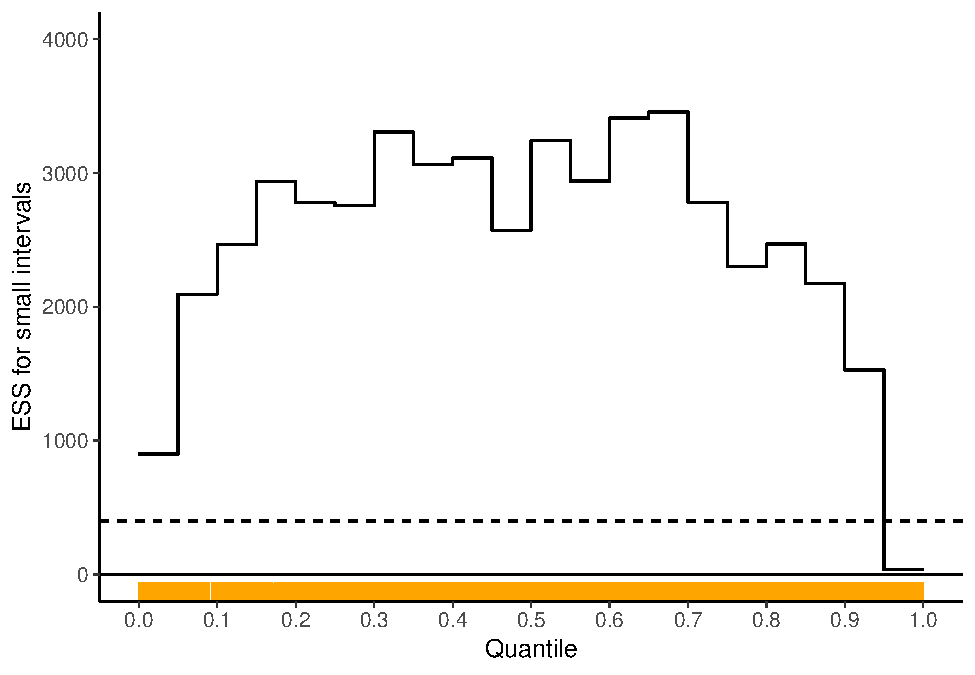
\includegraphics[width=0.6\linewidth]{graphics/local-ess-fit-nom-1.pdf}
  \caption{The local efficiency of small interval probability
    estimates for Cauchy model with nominal parameterization. Orange
    ticks show iterations that exceeded the maximum treedepth in
    dynamic HMC algorithm.}
\label{fig:local-ess-fit-nom-1}
\end{figure}
The efficiency of sampling is worryingly low in the tails (which is
caused by slow mixing in long tails of Cauchy).  
%
Figure~\ref{fig:quantile-ess-fit-nom-1} shows the efficiency
of quantile estimates (see Section
\protect\hyperlink{quantile_S_eff}{Efficiency for quantiles}).
\begin{figure}[tp]
  \centering
  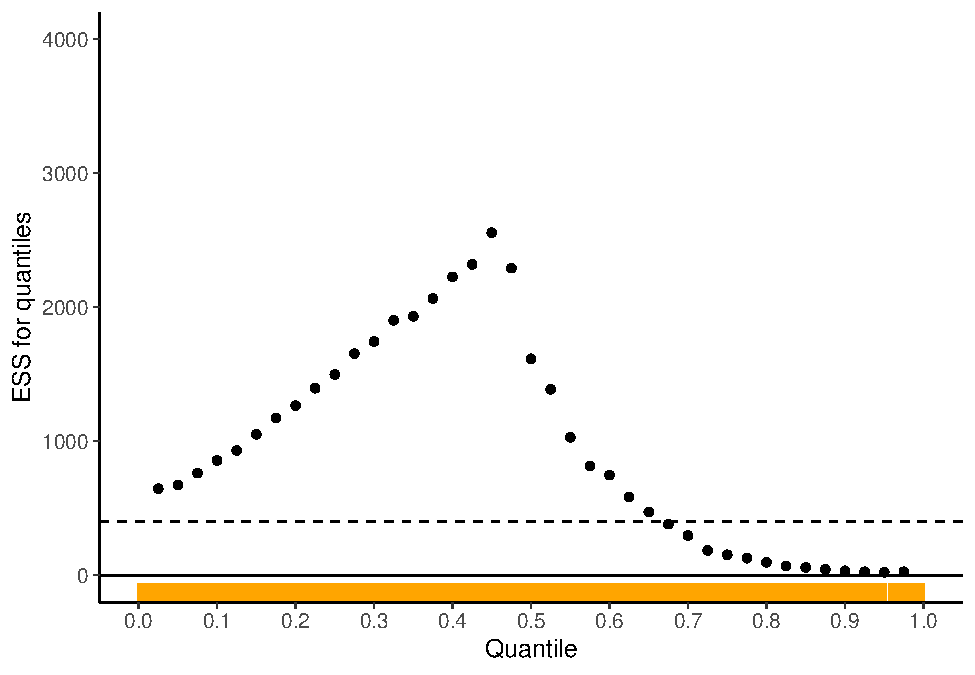
\includegraphics[width=0.6\linewidth]{graphics/quantile-ess-fit-nom-1.pdf}
  \caption{The efficiency of quantile estimates for Cauchy model with nominal parameterization.}
  \label{fig:quantile-ess-fit-nom-1}
\end{figure}
Similar as above, the sampling efficiency is worryingly low in the
tails. 

We may also investigate how the estimated effective sample sizes
change when we use more and more draws (\citet{Brooks+Gelman:1998}
proposed to use similar graph for \(\widehat{R}\)). If the effective
sample size is highly unstable, does not increase proportionally with
more draws, or even decreases, this indicates that simply running
longer chains will likely not solve the convergence issues. In
Figure~\ref{fig:change-ess-fit-nom-1}, we see how unstable both
bulk-ESS and tail-ESS are for this example.
\begin{figure}[tp]
  \centering
  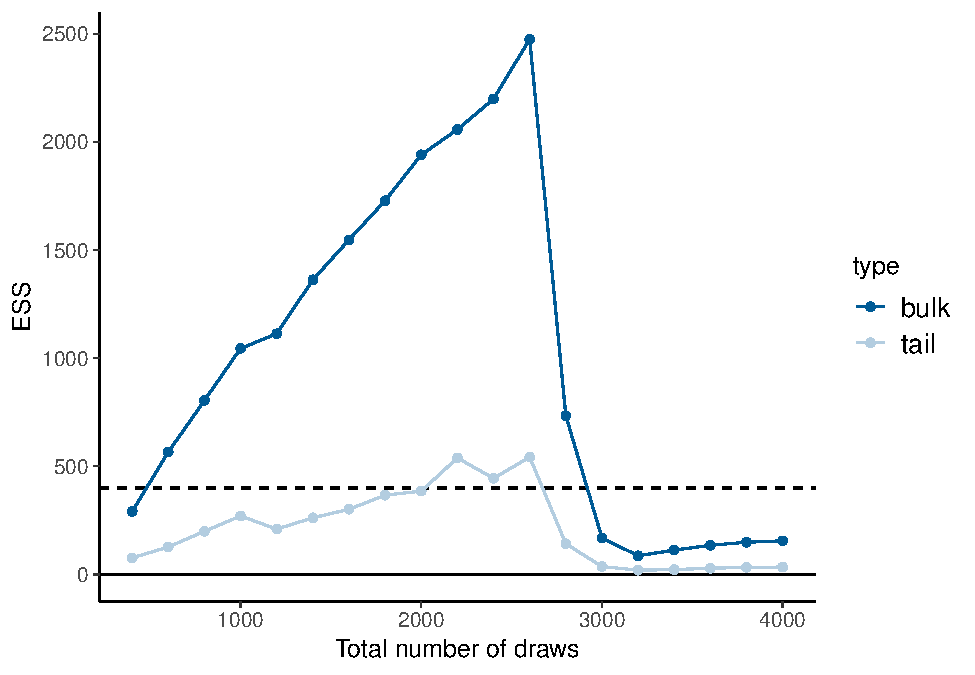
\includegraphics[width=0.6\linewidth]{graphics/change-ess-fit-nom-1.pdf}
  \caption{The estimated effective sample sizes with increasing number of iterations for Cauchy model with nominal parameterization.}
  \label{fig:change-ess-fit-nom-1}
\end{figure}
Rank plots in Figure~\ref{fig:hist-fit-nom-1} clearly show the
mixing problem between chains. In case of good mixing all rank plots
should be close to uniform.
\begin{figure}[tp]
  \centering
  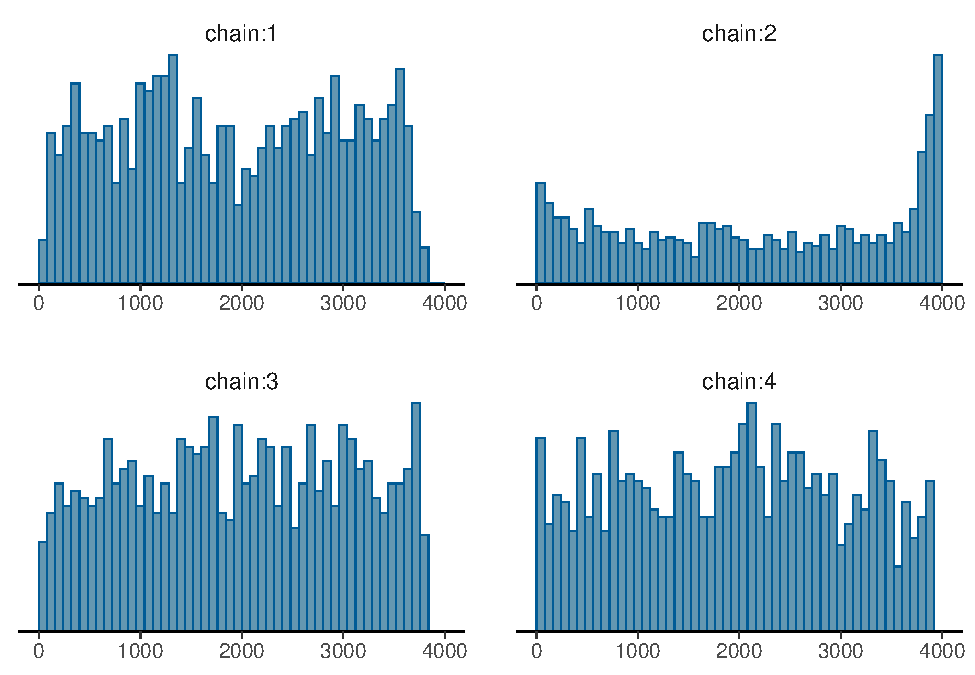
\includegraphics[width=0.6\linewidth]{graphics/hist-fit-nom-1.pdf}
  \caption{Rank plots of posterior draws from four chains for Cauchy model with nominal parameterization.}
  \label{fig:hist-fit-nom-1}
\end{figure}

\hypertarget{alternative-parameterization-of-cauchy}{%
\subsubsection{Alternative parameterization of
Cauchy}\label{alternative-parameterization-of-cauchy}}

Next we examine an alternative parameterization that considers the
Cauchy distribution as a scale mixture of Gaussian distributions
\begin{align}
  a \sim  \N(0,1), \qquad
  b \sim  \Gam\left(\frac{1}{2},\frac{1}{2}\right), \qquad
  x =  \frac{a}{\sqrt{b}}.
\end{align}
The model has two parameters and the Cauchy distributed \(x\)'s can be
computed from those. In addition to improved sampling performance, the
example illustrates that focusing on diagnostics matters.

We set define 50 dimensional parameter vectors $a$ and $b$ from which
50 dimensional quantity $x$ is computed.
We use dynamic HMC and run 4 chains each with 1000 iterations of
warmup and 1000 iterations stored. There are no warnings, and the
sampling is much faster.

% \begin{verbatim}
% parameters {
%   vector[50] x_a;
%   vector<lower=0>[50] x_b;
% }

% transformed parameters {
%   vector[50] x = x_a ./ sqrt(x_b);
% }

% model {
%   x_a ~ normal(0, 1);
%   x_b ~ gamma(0.5, 0.5);
% }

% generated quantities {
%   real I = fabs(x[1]) < 1 ? 1 : 0;
% }
% \end{verbatim}

% Run the alternative model:


% \begin{verbatim}
% Inference for the input samples (4 chains: each with iter = 2000; warmup = 1000):

%             Q5    Q50    Q95    Mean      SD  Rhat Bulk_ESS Tail_ESS
% x_a[1]   -1.65  -0.02   1.66   -0.01    0.99  1.00     4361     2961
% x_a[2]   -1.67   0.00   1.63   -0.01    1.01  1.00     4015     3167
% x_a[3]   -1.66  -0.03   1.62   -0.01    1.00  1.00     4190     3013
% x_a[4]   -1.63  -0.01   1.69    0.01    1.01  1.00     3626     2822
% x_a[5]   -1.64  -0.01   1.58   -0.01    0.98  1.00     3447     3029
% x_a[6]   -1.62  -0.01   1.56   -0.01    0.97  1.00     3975     2795
% x_a[7]   -1.61   0.00   1.65    0.01    1.01  1.00     3919     2271
% x_a[8]   -1.67  -0.03   1.60   -0.02    1.01  1.00     3736     3040
% x_a[9]   -1.63  -0.04   1.55   -0.03    0.99  1.00     3852     3075
% x_a[10]  -1.66  -0.03   1.74    0.00    1.02  1.00     3457     2810
% x_a[11]  -1.56  -0.02   1.55   -0.01    0.97  1.00     3532     2822
% x_a[12]  -1.64   0.00   1.69    0.01    1.00  1.00     3462     3036
% x_a[13]  -1.59   0.01   1.63    0.01    0.99  1.00     3479     2764
% x_a[14]  -1.72  -0.03   1.63   -0.03    1.01  1.00     3872     3179
% x_a[15]  -1.65   0.02   1.70    0.02    1.02  1.00     3843     2855
% x_a[16]  -1.67  -0.01   1.62   -0.01    1.01  1.00     3610     3047
% x_a[17]  -1.63  -0.01   1.66   -0.01    0.99  1.00     4363     3076
% x_a[18]  -1.65  -0.01   1.69   -0.01    1.01  1.00     4636     3088
% x_a[19]  -1.61  -0.02   1.59   -0.02    0.98  1.00     4055     3037
% x_a[20]  -1.64  -0.01   1.62    0.00    1.00  1.00     4340     2792
% x_a[21]  -1.67   0.04   1.68    0.02    1.03  1.00     3628     2719
% x_a[22]  -1.63  -0.01   1.64   -0.01    1.01  1.00     3976     2775
% x_a[23]  -1.62   0.03   1.70    0.02    1.01  1.00     4266     2682
% x_a[24]  -1.66   0.00   1.67    0.00    1.00  1.00     3710     2889
% x_a[25]  -1.64   0.02   1.66    0.00    1.00  1.00     4408     3062
% x_a[26]  -1.65  -0.02   1.61    0.00    1.00  1.00     3854     2674
% x_a[27]  -1.66   0.00   1.68    0.00    1.01  1.00     3331     2944
% x_a[28]  -1.69   0.02   1.68    0.02    1.01  1.00     4055     2689
% x_a[29]  -1.57   0.00   1.64    0.02    0.99  1.00     4097     3213
% x_a[30]  -1.61   0.00   1.64    0.01    0.99  1.00     3961     2900
% x_a[31]  -1.65   0.01   1.61    0.00    0.99  1.00     4097     3088
% x_a[32]  -1.59  -0.01   1.59   -0.01    0.97  1.00     4189     3171
% x_a[33]  -1.69  -0.01   1.77    0.00    1.05  1.00     3853     2594
% x_a[34]  -1.68   0.01   1.69    0.00    1.01  1.00     4012     2787
% x_a[35]  -1.61   0.03   1.67    0.03    1.00  1.00     3920     2829
% x_a[36]  -1.67   0.00   1.60   -0.01    0.99  1.00     4107     2797
% x_a[37]  -1.69  -0.03   1.59   -0.02    1.00  1.00     3956     2942
% x_a[38]  -1.67  -0.02   1.64   -0.02    1.02  1.00     4210     2919
% x_a[39]  -1.66  -0.02   1.65   -0.02    1.02  1.00     4482     2869
% x_a[40]  -1.63   0.00   1.62    0.00    1.00  1.00     4139     2848
% x_a[41]  -1.68   0.02   1.61    0.00    0.99  1.00     3963     2962
% x_a[42]  -1.64   0.03   1.64    0.02    1.00  1.00     4161     3077
% x_a[43]  -1.64  -0.03   1.63   -0.02    1.01  1.00     3808     2849
% x_a[44]  -1.66  -0.03   1.63   -0.02    1.00  1.00     3743     2865
% x_a[45]  -1.68   0.02   1.73    0.01    1.02  1.00     3783     2546
% x_a[46]  -1.56   0.04   1.66    0.05    0.97  1.00     4340     3277
% x_a[47]  -1.66   0.02   1.58    0.00    1.00  1.00     4283     2946
% x_a[48]  -1.61   0.00   1.66    0.00    0.98  1.00     4001     2779
% x_a[49]  -1.62   0.00   1.64    0.00    1.00  1.00     3906     3099
% x_a[50]  -1.62  -0.01   1.58    0.00    0.99  1.00     3794     2962
% x_b[1]    0.00   0.44   4.00    1.00    1.44  1.00     2268     1264
% x_b[2]    0.00   0.46   3.75    1.00    1.38  1.00     2444     1428
% x_b[3]    0.00   0.47   3.89    1.03    1.46  1.00     3578     1950
% x_b[4]    0.00   0.46   3.83    1.01    1.41  1.00     2693     1342
% x_b[5]    0.00   0.45   3.95    1.03    1.46  1.00     3056     1731
% x_b[6]    0.00   0.44   3.80    1.00    1.41  1.00     3264     1786
% x_b[7]    0.01   0.43   3.62    0.95    1.32  1.00     2888     1907
% x_b[8]    0.00   0.44   3.79    1.01    1.40  1.00     2876     1578
% x_b[9]    0.00   0.50   3.67    1.00    1.36  1.00     2820     1535
% x_b[10]   0.00   0.44   3.79    0.99    1.39  1.00     2534     1699
% x_b[11]   0.01   0.49   3.90    1.03    1.44  1.00     3595     2032
% x_b[12]   0.00   0.44   3.82    0.99    1.40  1.00     2405     1200
% x_b[13]   0.00   0.46   3.97    1.03    1.45  1.00     2045     1073
% x_b[14]   0.00   0.44   3.97    1.03    1.49  1.00     2829     1443
% x_b[15]   0.01   0.45   3.77    1.01    1.41  1.00     2853     1447
% x_b[16]   0.00   0.48   3.79    1.01    1.43  1.00     2661     1604
% x_b[17]   0.01   0.46   3.93    1.02    1.42  1.00     2775     1477
% x_b[18]   0.01   0.50   4.11    1.06    1.53  1.00     2689     1170
% x_b[19]   0.00   0.45   3.92    1.00    1.41  1.00     2392     1450
% x_b[20]   0.00   0.42   3.96    0.99    1.42  1.00     2296     1240
% x_b[21]   0.01   0.49   3.94    1.04    1.43  1.00     3069     1848
% x_b[22]   0.00   0.45   3.95    1.02    1.46  1.00     3012     1733
% x_b[23]   0.00   0.46   3.95    1.00    1.42  1.00     1787     1093
% x_b[24]   0.00   0.44   3.86    1.00    1.43  1.00     1903     1008
% x_b[25]   0.00   0.45   3.66    0.98    1.39  1.00     2348     1094
% x_b[26]   0.00   0.47   4.05    1.03    1.46  1.00     2421     1549
% x_b[27]   0.00   0.45   3.90    1.01    1.41  1.00     2777     1470
% x_b[28]   0.00   0.46   3.79    0.98    1.37  1.00     3353     1699
% x_b[29]   0.01   0.46   3.87    1.01    1.43  1.00     3428     1997
% x_b[30]   0.00   0.44   3.89    1.01    1.43  1.00     2833     1554
% x_b[31]   0.00   0.49   3.84    1.01    1.41  1.00     3035     1633
% x_b[32]   0.00   0.43   3.75    0.97    1.36  1.00     2276     1602
% x_b[33]   0.00   0.45   3.79    1.00    1.41  1.00     3093     1888
% x_b[34]   0.00   0.47   3.97    1.03    1.45  1.00     3309     1650
% x_b[35]   0.00   0.48   3.84    1.02    1.42  1.00     2493     1588
% x_b[36]   0.00   0.44   3.89    0.99    1.39  1.00     3108     1876
% x_b[37]   0.00   0.46   3.70    0.98    1.35  1.00     2644     1322
% x_b[38]   0.01   0.45   3.93    1.01    1.45  1.00     3155     1776
% x_b[39]   0.00   0.45   3.75    0.99    1.42  1.00     2038      934
% x_b[40]   0.00   0.42   3.76    0.94    1.31  1.00     2657     1403
% x_b[41]   0.00   0.46   3.78    1.00    1.38  1.00     2648     1370
% x_b[42]   0.00   0.45   3.89    1.00    1.43  1.00     2334     1365
% x_b[43]   0.00   0.47   4.03    1.03    1.44  1.00     2967     1797
% x_b[44]   0.00   0.43   3.69    0.97    1.37  1.00     2557     1591
% x_b[45]   0.00   0.44   3.66    0.96    1.30  1.00     2731     1785
% x_b[46]   0.00   0.46   3.74    1.01    1.40  1.00     2538     1183
% x_b[47]   0.01   0.47   3.83    1.01    1.39  1.00     3948     2071
% x_b[48]   0.01   0.48   3.89    1.02    1.39  1.00     3207     1917
% x_b[49]   0.00   0.47   3.74    1.00    1.35  1.00     2550     1533
% x_b[50]   0.00   0.46   4.01    1.00    1.48  1.00     2881     1395
% x[1]     -6.47  -0.02   6.52    0.01   34.90  1.01     3901     2122
% x[2]     -6.52   0.00   6.50    3.39  146.00  1.00     3767     1947
% x[3]     -6.31  -0.03   5.95   -0.08   16.20  1.00     3681     2514
% x[4]     -6.76  -0.01   5.86   -1.26   50.70  1.00     3244     2159
% x[5]     -6.67  -0.01   5.75   -0.31   30.30  1.00     3355     2430
% x[6]     -5.64  -0.01   6.48 -146.00 6460.00  1.00     3802     2536
% x[7]     -6.59   0.00   6.37   -0.58   22.60  1.00     3480     2508
% x[8]     -6.50  -0.04   6.29   -0.04   20.60  1.00     3474     2374
% x[9]     -5.73  -0.04   5.96   -0.92   55.60  1.00     3493     2262
% x[10]    -6.37  -0.04   6.43   -0.20   25.20  1.00     2871     2286
% x[11]    -5.61  -0.02   5.55    0.12   12.40  1.00     3423     2587
% x[12]    -7.12   0.00   6.19    0.41   91.80  1.00     3340     2329
% x[13]    -6.44   0.02   6.22   -5.65  202.00  1.00     3332     2164
% x[14]    -6.72  -0.04   6.56   -2.94  135.00  1.00     3693     2257
% x[15]    -5.68   0.02   6.06   -0.86   30.40  1.00     3511     1969
% x[16]    -6.99  -0.01   7.24   -0.40   24.60  1.00     3614     2406
% x[17]    -5.78  -0.01   5.39   -0.06   25.10  1.00     3880     2520
% x[18]    -5.45  -0.01   5.92   -0.55  259.00  1.00     4303     2254
% x[19]    -7.16  -0.02   5.84    9.85  549.00  1.00     3505     1931
% x[20]    -7.39  -0.01   6.68   -3.09  146.00  1.00     3411     1916
% x[21]    -5.93   0.05   5.85    0.23   45.60  1.00     3419     2179
% x[22]    -6.96  -0.02   6.23   -0.20   27.10  1.00     3554     2149
% x[23]    -5.99   0.05   6.54    2.51  115.00  1.00     3456     2098
% x[24]    -6.75   0.00   6.99   -0.67  111.00  1.00     3541     1922
% x[25]    -6.33   0.02   6.40   -2.71  100.00  1.00     4036     2356
% x[26]    -5.57  -0.02   6.32    0.20   14.50  1.00     3335     2319
% x[27]    -6.40   0.00   6.17   -0.78   52.60  1.00     3377     2400
% x[28]    -5.70   0.02   6.49    3.10  105.00  1.00     3446     2121
% x[29]    -5.40   0.00   5.67   -0.12   18.10  1.00     3918     2430
% x[30]    -5.83  -0.01   6.45    1.00   51.20  1.00     3642     2138
% x[31]    -5.85   0.02   5.66    0.86   26.30  1.00     3595     2271
% x[32]    -6.49  -0.01   6.18    0.11   50.70  1.00     4227     2731
% x[33]    -7.08  -0.01   6.34   -0.41   23.50  1.00     3807     2376
% x[34]    -6.59   0.01   6.05    0.95   48.20  1.00     4084     2358
% x[35]    -5.44   0.03   6.13    0.32   48.40  1.00     3756     2247
% x[36]    -6.15   0.00   6.11   -0.06   28.40  1.00     3600     2386
% x[37]    -6.08  -0.03   5.34    0.70   59.90  1.00     3623     2005
% x[38]    -5.74  -0.02   5.77    0.20   13.20  1.00     3820     2536
% x[39]    -6.73  -0.03   5.84    2.77  285.00  1.00     4121     1944
% x[40]    -6.39   0.01   6.52   -2.75  103.00  1.00     3612     1823
% x[41]    -6.01   0.02   5.92   -0.42   35.70  1.00     3492     2222
% x[42]    -7.39   0.05   6.86    0.49   22.50  1.00     3558     1949
% x[43]    -5.98  -0.03   6.69   14.40  626.00  1.00     3823     2516
% x[44]    -7.04  -0.04   6.17    1.55  106.00  1.00     3310     2239
% x[45]    -5.75   0.02   6.23   -0.43   32.30  1.00     3752     2437
% x[46]    -5.59   0.06   6.33   -0.32   76.00  1.00     3898     1976
% x[47]    -5.49   0.03   5.43   -0.02   12.10  1.00     3893     2659
% x[48]    -5.96   0.00   4.85   -0.01   21.00  1.00     3674     2274
% x[49]    -6.55   0.00   5.25   -1.24  129.00  1.00     3576     2243
% x[50]    -6.74  -0.01   6.90   -1.06  147.00  1.00     3437     2486
% I         0.00   0.00   1.00    0.50    0.50  1.00     2648     4000
% lp__    -95.20 -81.00 -68.70  -81.30    8.08  1.00     1310     1928

% For each parameter, Bulk_ESS and Tail_ESS are crude measures of 
% effective sample size for bulk and tail quantities respectively (good values is 
% ESS > 400), and Rhat is the potential scale reduction factor on rank normalized
% split chains (at convergence, Rhat = 1).
% \end{verbatim}

All \emph{split}-\(\widehat{R}<1.01\) and ESS\(>400\) indicate the
sampling worked much better with the alternative parameterization.
Oneline appendix has more results using other
alternative parameterizations. The \(a\) and \(b\) used
to form the Cauchy distributed \(x\) have stable quantile, mean and
sd values. As \(x\) is Cauchy distributed it has stable
quantiles, but wildly varying mean and sd estimates as the true values
are not finite.
%
We can further analyze potential problems using local efficiency
estimates and rank plots. We take a detailed look at \(x_{40}\), which
has the smallest bulk-ESS of 2848.
%
Figure~\ref{fig:local-ess-fit-alt1-1} shows
the local efficiency of small interval probability estimates.
\begin{figure}[tp]
  \centering
  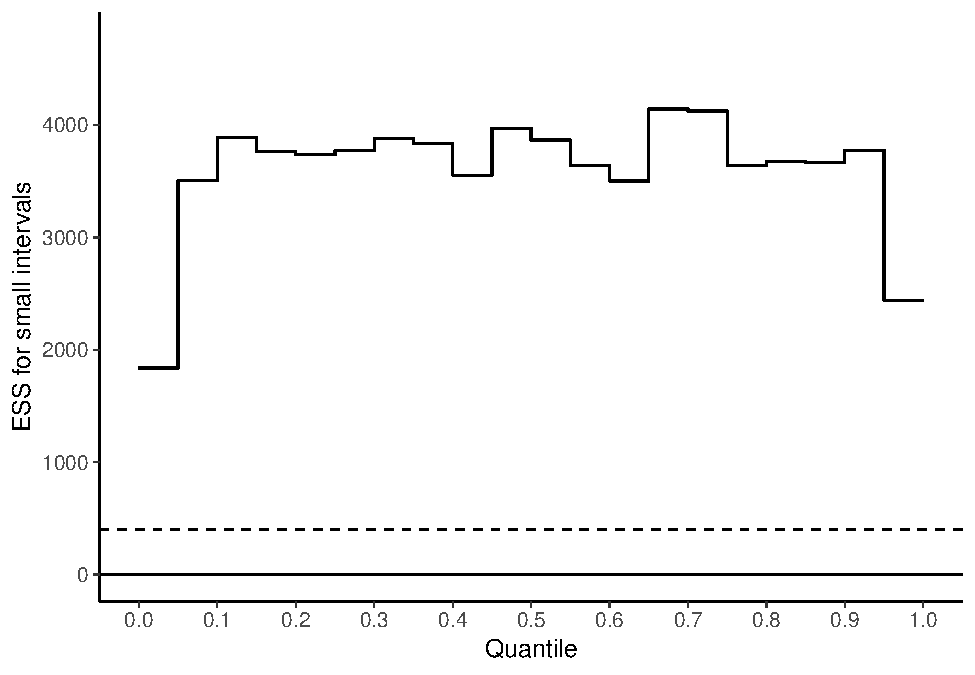
\includegraphics[width=0.6\linewidth]{graphics/local-ess-fit-alt1-1.pdf}
  \caption{The local efficiency of small interval probability estimates for Cauchy model with alternative parameterization.}
\label{fig:local-ess-fit-alt1-1}
\end{figure}
Figure~\ref{fig:quantile-ess-alt1-1} shows also the good sampling efficiency
of quantile estimates.
\begin{figure}[tp]
  \centering
  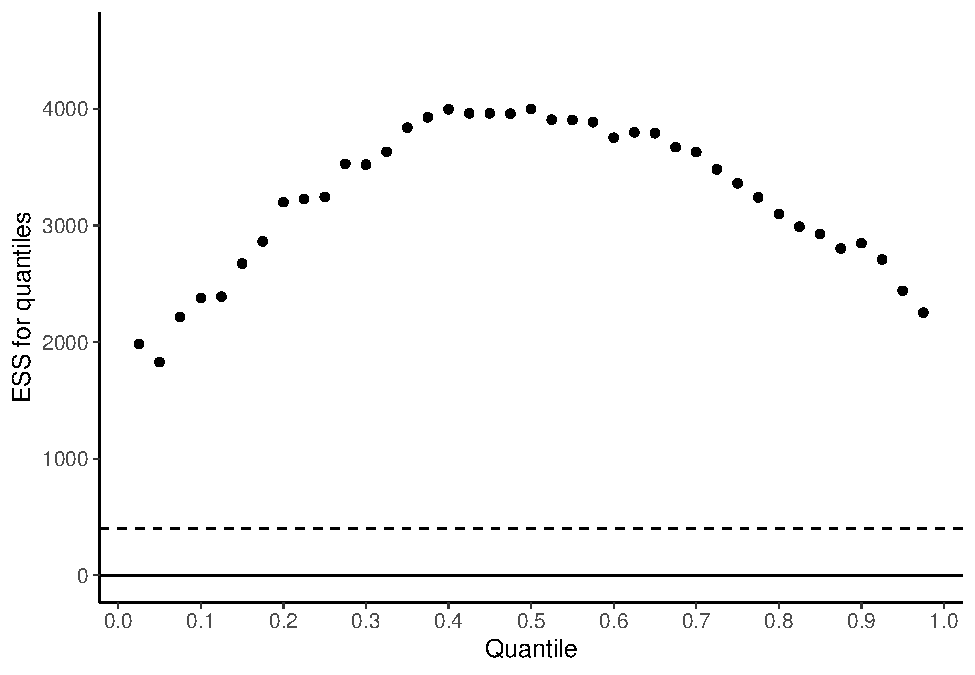
\includegraphics[width=0.6\linewidth]{graphics/quantile-ess-fit-alt1-1.pdf}
  \caption{The efficiency of quantile estimates for Cauchy model with alternative parameterization.}
  \label{fig:quantile-ess-alt1-1}
\end{figure}
%
Rank plots in Figure~\ref{fig:hist-fit-alt1-1} also look quite uniform across chains.
\begin{figure}[tp]
  \centering
  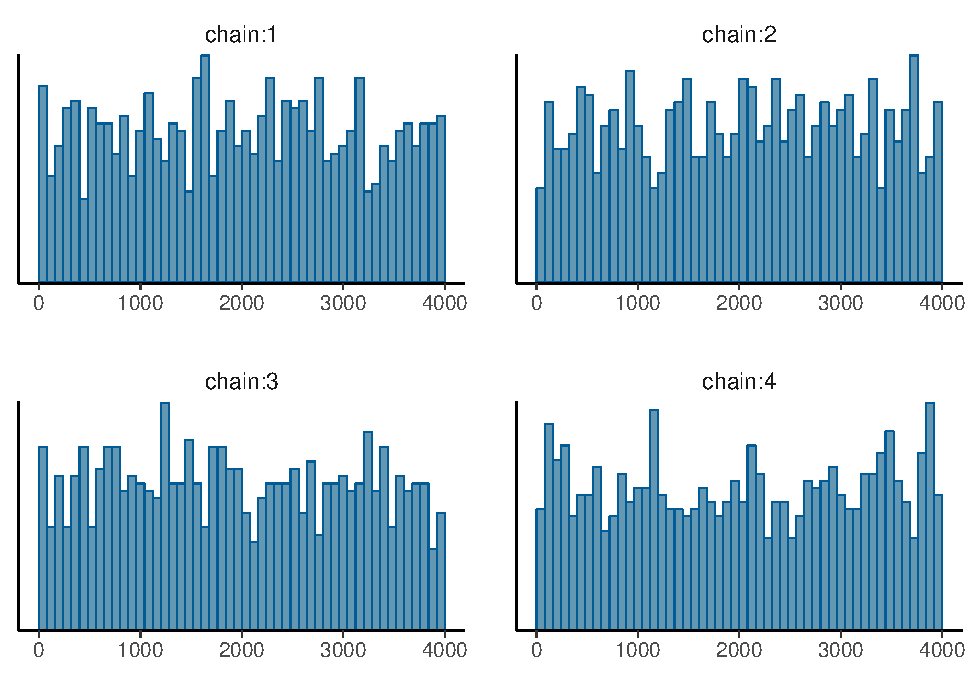
\includegraphics[width=0.6\linewidth]{graphics/hist-fit-alt1-1.pdf}
  \caption{Rank plots of posterior draws from four chains for Cauchy model with alternative parameterization.}
  \label{fig:hist-fit-alt1-1}
\end{figure}

In summary, the alternative parameterization produces results that look
much better than for the nominal parameterization.

\hypertarget{half-cauchy-with-nominal-parameterization}{%
\subsubsection{Half-Cauchy with nominal
parameterization}\label{half-cauchy-with-nominal-parameterization}}

Half-Cauchy priors are common and, for example, in Stan usually set
using the nominal parameterization
\begin{align}
  x \sim \Cauchy^+(0,1).
\end{align}
However, when the constraint \texttt{\textless{}lower=0\textgreater{}}
is used, Stan does the sampling automatically in the unconstrained
\(\log(x)\) space, which changes the geometry crucially.

We set independent half-Cauchy distribution for 50 dimensional vector
$x$ with automatic transformation so that sampling is done in
\(\log(x)\) space.  We use dynamic HMC and run 4 chains each with 1000
iterations of warmup and 1000 iterations stored.  There are no
warnings, and the sampling is much faster than for the Cauchy nominal
model.


% \begin{verbatim}
% parameters {
%   vector<lower=0>[50] x;
% }

% model {
%   x ~ cauchy(0, 1);
% }

% generated quantities {
%   real I = fabs(x[1]) < 1 ? 1 : 0;
% }
% \end{verbatim}

% Run the half-Cauchy with nominal parameterization (and positive
% constraint):


% \begin{verbatim}
% Inference for the input samples (4 chains: each with iter = 2000; warmup = 1000):

%           Q5    Q50   Q95   Mean      SD  Rhat Bulk_ESS Tail_ESS
% x[1]    0.08   1.03  13.6  11.10  388.00     1     8077     2223
% x[2]    0.10   1.02  10.8  11.60  482.00     1     9868     2612
% x[3]    0.06   1.00  12.9   5.40   71.60     1     7895     2097
% x[4]    0.09   0.98  11.5   4.41   29.50     1     7596     2347
% x[5]    0.08   1.03  14.0   4.52   19.80     1     7495     2230
% x[6]    0.08   0.99  11.7  12.50  380.00     1     7948     2145
% x[7]    0.07   0.98  12.0   9.23  281.00     1     8336     2117
% x[8]    0.09   0.99  10.8   4.61   40.80     1     8194     2165
% x[9]    0.09   1.02  11.6  11.70  483.00     1     8464     2127
% x[10]   0.07   1.03  14.9   6.01   51.00     1     7963     2399
% x[11]   0.08   0.97  12.5  15.60  532.00     1     6980     1788
% x[12]   0.07   1.03  13.3   4.10   17.50     1     8226     2029
% x[13]   0.08   1.01  14.1   8.88  120.00     1     8077     2032
% x[14]   0.07   0.96  13.5   6.91   71.50     1     7455     2261
% x[15]   0.07   1.00  14.4   8.66   95.80     1     6766     2246
% x[16]   0.08   0.99  14.1   5.55   38.40     1     7396     2174
% x[17]   0.08   0.99  11.7   8.70  300.00     1     7144     2260
% x[18]   0.09   0.98  11.6  14.40  398.00     1     7614     2035
% x[19]   0.07   0.99  14.3   6.33   69.10     1     7823     1825
% x[20]   0.09   1.00  11.2   6.40  160.00     1     7905     2355
% x[21]   0.07   1.00  12.0   7.03  144.00     1     7843     2078
% x[22]   0.09   1.02  12.7  32.20 1730.00     1     7735     2043
% x[23]   0.07   0.98  13.5   6.33   67.30     1     7119     2142
% x[24]   0.07   1.00  12.3   4.99   41.60     1     6893     1982
% x[25]   0.09   1.00  11.5   8.60  270.00     1     7757     2351
% x[26]   0.08   0.98  10.7   6.97  119.00     1     6433     2230
% x[27]   0.08   1.01  13.4   4.88   34.30     1     7005     2119
% x[28]   0.08   0.97  11.4   5.76   66.70     1     9631     2228
% x[29]   0.07   1.00  13.7  10.40  240.00     1     6109     2312
% x[30]   0.09   1.02  11.0   7.98  206.00     1     7958     2368
% x[31]   0.08   0.96  12.4   4.39   32.10     1     6493     2102
% x[32]   0.10   1.01  11.5   4.99   55.40     1     7043     1742
% x[33]   0.08   0.99  13.8   5.45   36.80     1     6913     2455
% x[34]   0.08   0.98  12.4   5.92   78.20     1     8610     2514
% x[35]   0.07   0.96  13.6   5.70   57.40     1     6406     2160
% x[36]   0.06   1.00  13.5   5.36   39.60     1     7694     2031
% x[37]   0.07   1.00  13.9   8.29  196.00     1     7276     2491
% x[38]   0.08   1.02  12.2   6.40  119.00     1     6790     2369
% x[39]   0.10   1.01  11.7   6.67   88.50     1     7739     2518
% x[40]   0.09   0.96  12.1   5.16   44.40     1     7087     2349
% x[41]   0.07   0.96  12.9   4.97   42.30     1     8650     2333
% x[42]   0.07   1.02  13.3   7.77  132.00     1     8703     2410
% x[43]   0.08   0.97  10.2  26.60 1400.00     1     8747     2194
% x[44]   0.08   1.03  12.3   5.96   59.30     1     6378     2257
% x[45]   0.08   0.98  12.2   7.70  123.00     1     8430     2314
% x[46]   0.08   0.99  12.1   5.36   72.20     1     8185     2237
% x[47]   0.08   1.01  14.5   7.00   76.70     1     9562     2265
% x[48]   0.08   1.01  13.0   5.06   30.40     1     8402     2690
% x[49]   0.08   1.00  12.9   7.48  100.00     1     7993     1804
% x[50]   0.08   1.00  13.2   8.86  179.00     1     7523     2243
% I       0.00   0.00   1.0   0.49    0.50     1     7357     4000
% lp__  -80.60 -69.10 -59.3 -69.30    6.42     1     1218     2001

% For each parameter, Bulk_ESS and Tail_ESS are crude measures of 
% effective sample size for bulk and tail quantities respectively (good values is 
% ESS > 400), and Rhat is the potential scale reduction factor on rank normalized
% split chains (at convergence, Rhat = 1).
% \end{verbatim}

All \emph{split}-\(\widehat{R}<1.01\) and ESS\(>400\) indicate good
performance of the sampler. We see that the Stan's automatic (and
implicit) transformation of constraint parameters can have a big effect
on the sampling performance. More experiments with different
parameterizations of the half-Cauchy distribution can be found in
the online appendix.

%\FloatBarrier

\hypertarget{eightschools}{%
\subsection{Hierarchical model: Eight Schools}\label{eightschools}}

The Eight Schools data is a classic example for hierarchical models
\citep[see Section 5.5 in][]{BDA3}, which despite the apparent
simplicity nicely illustrates the typical problems in inference for
hierarchical models. The centered parameterization exhibits a funnel shape
that contracts into a region of strong curvature around small
values of population prior scale $\tau$, making it difficult for most Markov chain
methods to adequately explore.
Online appendix contains more detailed
analysis of different algorithm variants including also Gibbs sampling.

\hypertarget{a-centered-eight-schools-model}{%
\subsubsection{A Centered Eight Schools
model}\label{a-centered-eight-schools-model}}

We use dynamic HMC and run 4 chains each with 1000 iterations of
warmup and 1000 iterations stored. Instead of the default options, we
run the centered parameterization model with an increased
\texttt{adapt\_delta} value to reduce the probability of getting
divergent transitions. Despite an increased \texttt{adapt\_delta}, we
still observe a lot of divergent transitions, which in itself is
already sufficient indicator of convergence problems. We can use
\emph{split}-\(\widehat{R}\) and ESS diagnostics to recognize
problematic parts of the posterior, and they can be used also in cases
when other MCMC algorithms than HMC is used.

% \begin{verbatim}
% Inference for the input samples (4 chains: each with iter = 2000; warmup = 1000):

%              Q5    Q50   Q95   Mean   SD  Rhat Bulk_ESS Tail_ESS
% mu        -1.11   4.53  9.90   4.44 3.39  1.02      548      754
% tau        0.39   2.85  9.61   3.62 3.10  1.07       67       82
% theta[1]  -2.24   5.81 16.30   6.23 5.74  1.02      747     1294
% theta[2]  -2.60   5.07 13.40   5.08 4.86  1.01      970     1240
% theta[3]  -5.01   4.35 12.10   3.94 5.33  1.01      899     1147
% theta[4]  -2.86   5.00 12.80   4.89 4.82  1.01      986     1059
% theta[5]  -4.74   4.03 10.80   3.66 4.81  1.01      715      988
% theta[6]  -4.15   4.28 11.60   4.08 4.84  1.01      833      976
% theta[7]  -1.30   5.97 15.60   6.31 5.18  1.02      612     1182
% theta[8]  -3.37   5.12 13.80   4.98 5.34  1.01      901     1477
% lp__     -24.70 -15.00  0.37 -14.00 7.44  1.07       69       89

% For each parameter, Bulk_ESS and Tail_ESS are crude measures of 
% effective sample size for bulk and tail quantities respectively (good values is 
% ESS > 400), and Rhat is the potential scale reduction factor on rank normalized
% split chains (at convergence, Rhat = 1).
% \end{verbatim}

See online appendix for more details and results of longer chains.

Bulk-ESS and Tail-ESS for the between school standard deviation $\tau$
are 67 and 82 respectively. Both are less than 400, indicating we
should investigate that parameter more carefully. We thus examine the
local sampling efficiency in different parts of the posterior by
computing the efficiency estimate for small interval estimates.

Figures~\ref{fig:local-ess-fit-cp-1} and
\ref{fig:local-ess-fit-cp-norank-1} show the local efficiency of small
interval probability estimates with respect to ranks and parameter
values, respectively.
\begin{figure}[tp]
  \centering
  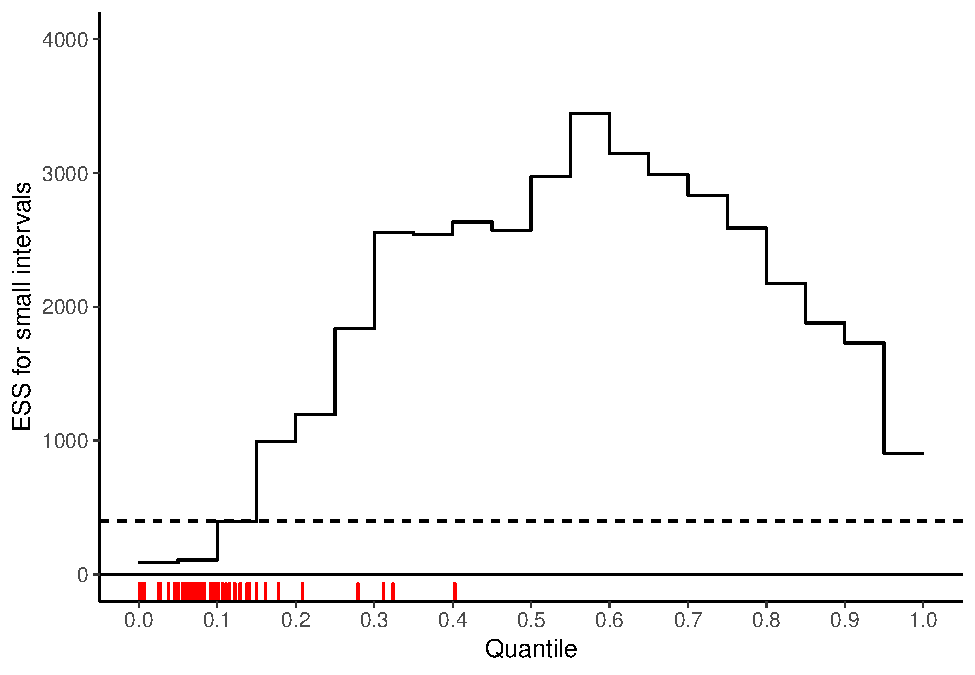
\includegraphics[width=0.6\linewidth]{graphics/local-ess-fit-cp-1.pdf}
  \caption{The local efficiency of small interval probability estimates for 8 schools model with centered parameterization. Red ticks show divergent transitions.}
  \label{fig:local-ess-fit-cp-1}
\end{figure}
\begin{figure}[tp]
  \centering
  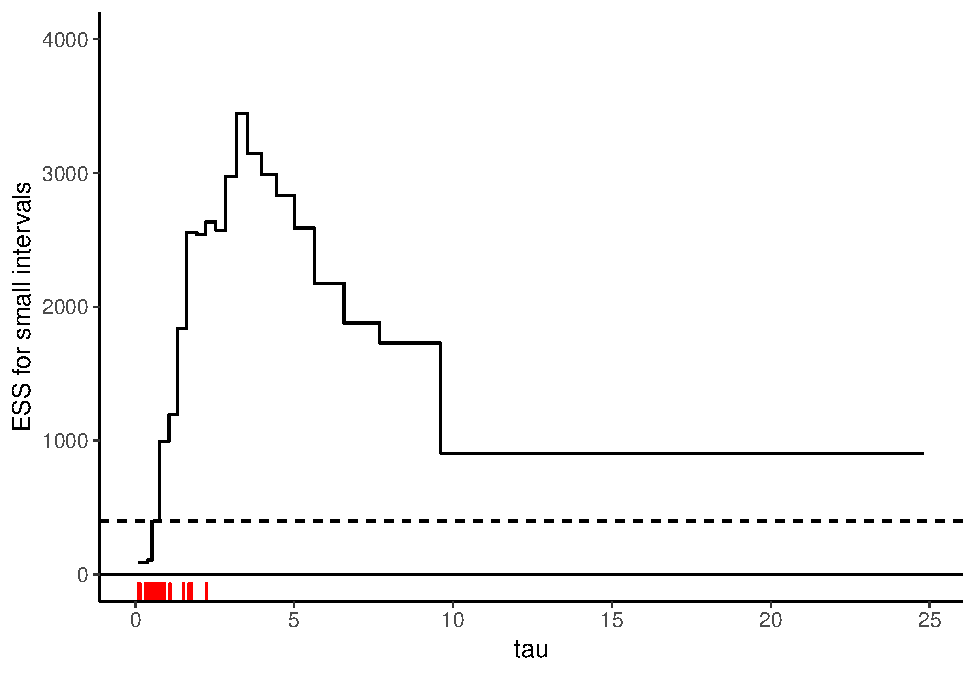
\includegraphics[width=0.6\linewidth]{graphics/local-ess-fit-cp-norank-1.pdf}
  \caption{The local efficiency of small interval probability estimates for 8 schools model with centered parameterization. Vertical axis is instead of ranks in scale of parameter $\tau$. Red ticks show divergent transitions.}
  \label{fig:local-ess-fit-cp-norank-1}
\end{figure}
The sampler has difficulties in exploring small $\tau$
values. As the sampling efficiency for estimating small $\tau$
values is practically zero, we may assume that we may miss substantial
amount of posterior mass and get biased estimates. Red ticks, which show
iterations with divergences, have concentrated to small $\tau$
values, indicate also problems exploring small values which is likely to
cause bias.
%
Figures~\ref{fig:quantile-ess-fit-cp-1}
and~\ref{fig:quantile-ess-fit-cp-norank-1} show corresponding
efficiency of quantile estimates with respect to ranks and parameter
values, respectively.
\begin{figure}[tp]
  \centering
  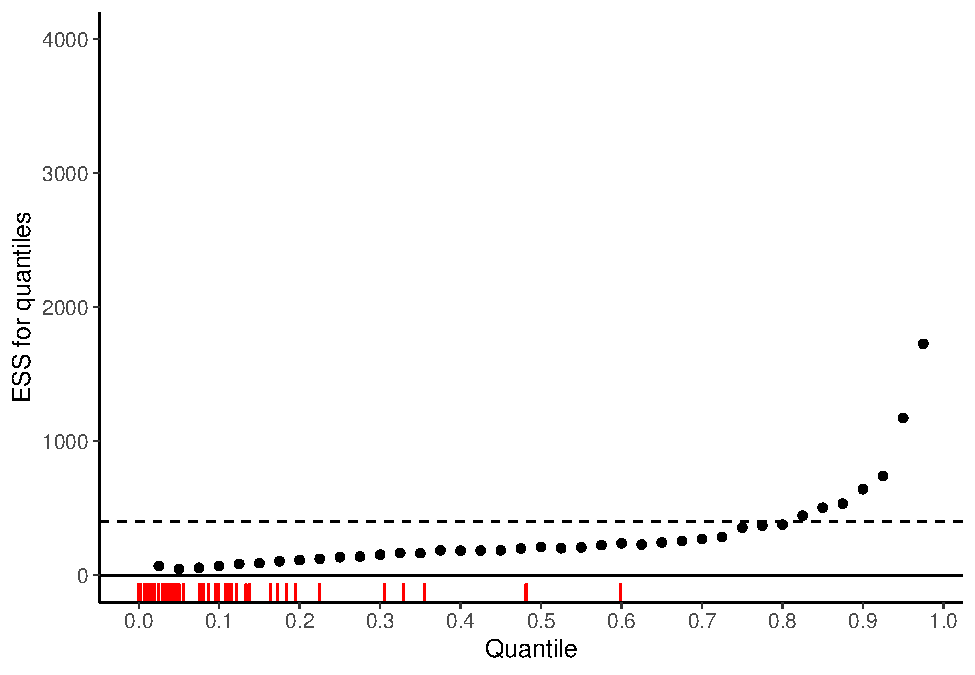
\includegraphics[width=0.6\linewidth]{graphics/quantile-ess-fit-cp-1.pdf}
  \caption{The efficiency of quantile estimates for 8 schools model with centered parameterization. Red ticks show divergent transitions.}
  \label{fig:quantile-ess-fit-cp-1}
\end{figure}
\begin{figure}[tp]
  \centering
  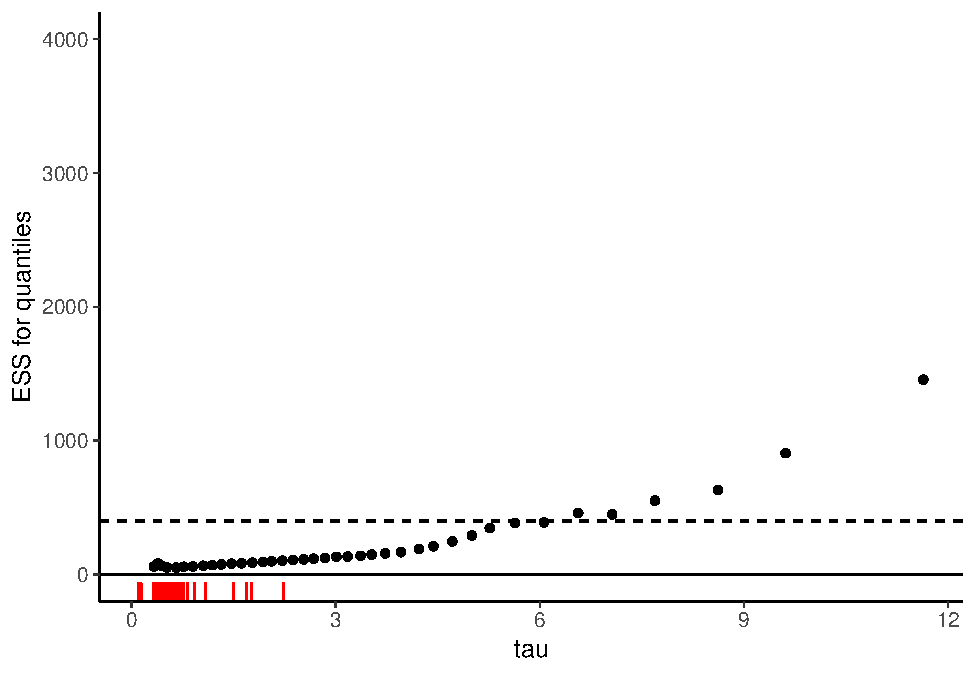
\includegraphics[width=0.6\linewidth]{graphics/quantile-ess-fit-cp-norank-1.pdf}
  \caption{The efficiency of quantile estimates for 8 schools model with centered parameterization. Vertical axis is instead of ranks in scale of parameter $\tau$. Red ticks show divergent transitions.}
  \label{fig:quantile-ess-fit-cp-norank-1}
\end{figure}
Most of the quantile estimates have worryingly low effective sample
size estimate.

Figure~\ref{fig:change-ess-fit-cp-1} shows how the estimated effective
sample sizes change when we use more and more draws.  Here we don't
see sudden changes, but both bulk-ESS and tail-ESS are low. See online
appendix for results of longer chains.
\begin{figure}[tp]
  \centering
  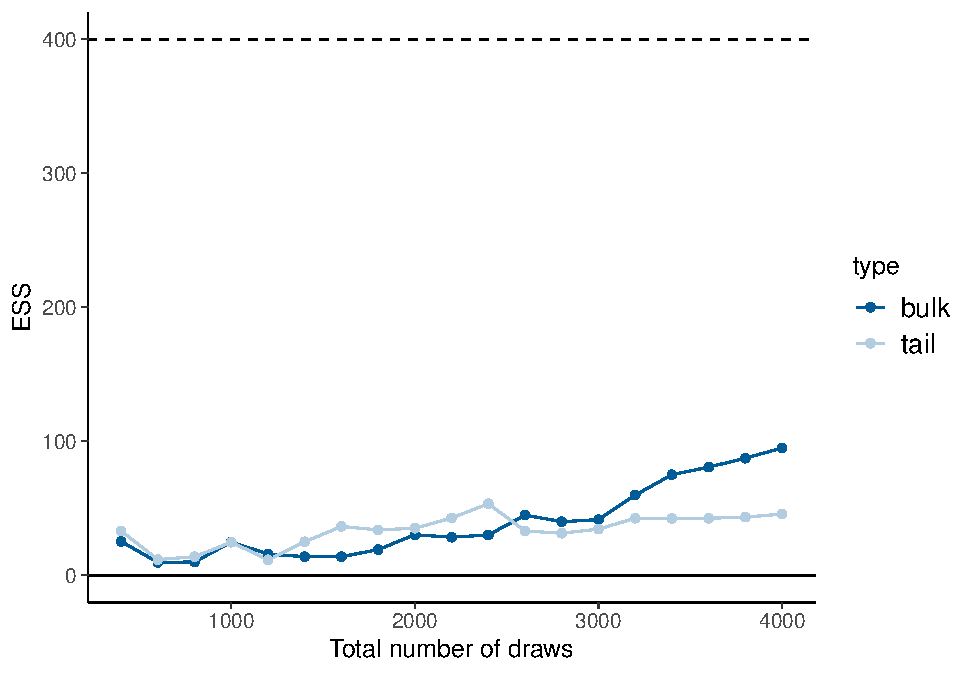
\includegraphics[width=0.6\linewidth]{graphics/change-ess-fit-cp-1.pdf}
  \caption{The estimated effective sample sizes with increasing number of iterations for 8 schools model with centered parameterization.}
  \label{fig:change-ess-fit-cp-1}
\end{figure}

In line with other findings, the rank plots of $\tau$ in
Figure~\ref{fig:hist-fit-cp-1} clearly show problems in the mixing of
the chains.
\begin{figure}[tp]
  \centering
  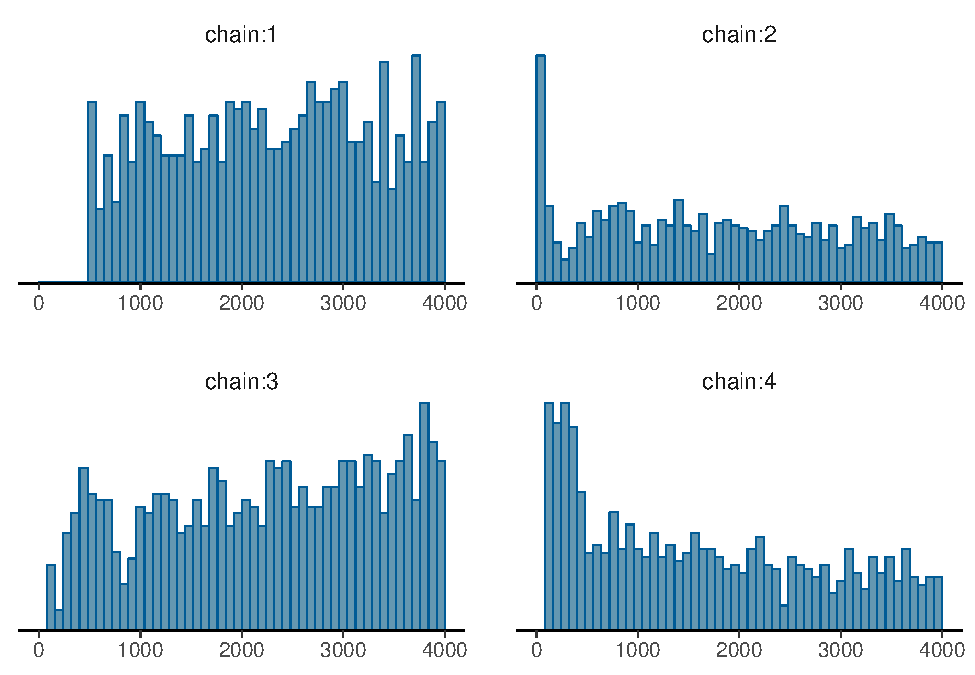
\includegraphics[width=0.6\linewidth]{graphics/hist-fit-cp-1.pdf}
  \caption{Rank plots of posterior draws from four chains for 8 schools model with centered parameterization.}
  \label{fig:hist-fit-cp-1}
\end{figure}

%\FloatBarrier

\hypertarget{non-centered-eight-schools-model}{%
\subsubsection{Non-centered Eight Schools
model}\label{non-centered-eight-schools-model}}

For hierarchical models, the corresponding non-centered
parameterization often works better.

% \begin{verbatim}
% data {
%   int<lower=0> J;
%   real y[J];
%   real<lower=0> sigma[J];
% }

% parameters {
%   real mu;
%   real<lower=0> tau;
%   real theta_tilde[J];
% }

% transformed parameters {
%   real theta[J];
%   for (j in 1:J)
%     theta[j] = mu + tau * theta_tilde[j];
% }

% model {
%   mu ~ normal(0, 5);
%   tau ~ cauchy(0, 5);
%   theta_tilde ~ normal(0, 1);
%   y ~ normal(theta, sigma);
% }
% \end{verbatim}

We use dynamic HMC and run 4 chains each with 1000 iterations of
warmup and 1000 iterations stored. For reasons of comparability, we
use the same \texttt{adapt\_delta} as for the centered
parameterization model. There are zero divergences and no other
warnings which is a first good sign.

% \begin{verbatim}
% Inference for the input samples (4 chains: each with iter = 2000; warmup = 1000):

%                    Q5   Q50   Q95  Mean   SD  Rhat Bulk_ESS Tail_ESS
% mu              -1.14  4.42  9.96  4.47 3.37     1     5531     3004
% tau              0.30  2.81  9.50  3.59 3.17     1     2872     1908
% theta_tilde[1]  -1.29  0.31  1.88  0.31 0.98     1     5046     2874
% theta_tilde[2]  -1.44  0.11  1.62  0.10 0.94     1     4177     2735
% theta_tilde[3]  -1.64 -0.08  1.48 -0.08 0.97     1     6485     2994
% theta_tilde[4]  -1.51  0.08  1.62  0.06 0.95     1     6076     2514
% theta_tilde[5]  -1.71 -0.17  1.39 -0.16 0.94     1     5608     3177
% theta_tilde[6]  -1.64 -0.06  1.53 -0.06 0.97     1     4855     2773
% theta_tilde[7]  -1.25  0.40  1.87  0.37 0.96     1     4796     2849
% theta_tilde[8]  -1.54  0.07  1.66  0.06 0.96     1     6142     2972
% theta[1]        -1.62  5.64 16.30  6.25 5.58     1     4907     3015
% theta[2]        -2.42  4.82 13.00  5.01 4.68     1     5122     3242
% theta[3]        -4.63  4.26 12.10  4.09 5.27     1     5457     3407
% theta[4]        -2.73  4.75 12.50  4.82 4.78     1     4695     3130
% theta[5]        -3.96  3.82 11.00  3.72 4.62     1     5346     3398
% theta[6]        -3.88  4.27 11.40  4.13 4.95     1     5670     3393
% theta[7]        -0.98  5.88 15.40  6.38 5.10     1     4708     3242
% theta[8]        -3.23  4.78 13.10  4.87 5.17     1     4924     3037
% lp__           -11.20 -6.60 -3.78 -6.92 2.31     1     1641     2344

% For each parameter, Bulk_ESS and Tail_ESS are crude measures of 
% effective sample size for bulk and tail quantities respectively (good values is 
% ESS > 400), and Rhat is the potential scale reduction factor on rank normalized
% split chains (at convergence, Rhat = 1).
% \end{verbatim}

All \emph{split}-\(\widehat{R}<1.01\) and ESS\(>400\) indicate a much
better efficiency of the non-centered parameterization.
%
We examine the sampling efficiency in different parts of the posterior
by computing the effective sample size for small interval probability
estimates for $\tau$.

Figures~\ref{fig:local-ess-fit-cp-1} and
\ref{fig:quantile-ess-fit-cp-1} show the efficiency of small interval
probability estimates and the efficiency of quantile estimates for
$\tau$.
\begin{figure}[tp]
  \centering
  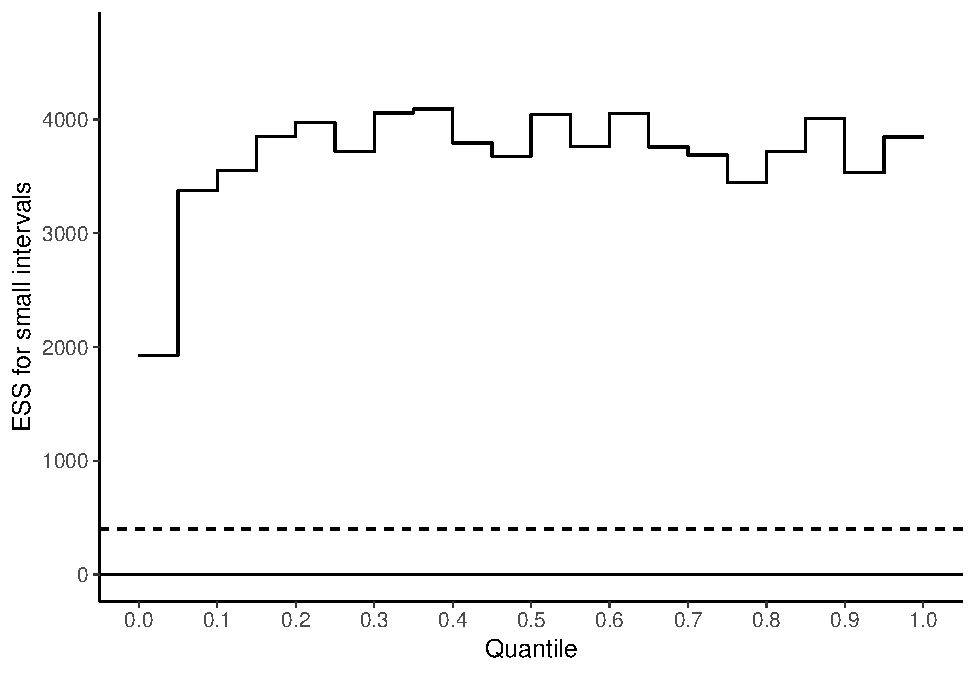
\includegraphics[width=0.6\linewidth]{graphics/local-ess-fit-ncp2-1.pdf}
  \caption{The local efficiency of small interval probability estimates for 8 schools model with non-centered parameterization.}
  \label{fig:local-ess-fit-ncp2-1}
\end{figure}
% \begin{figure}[tp]
%   \centering
%   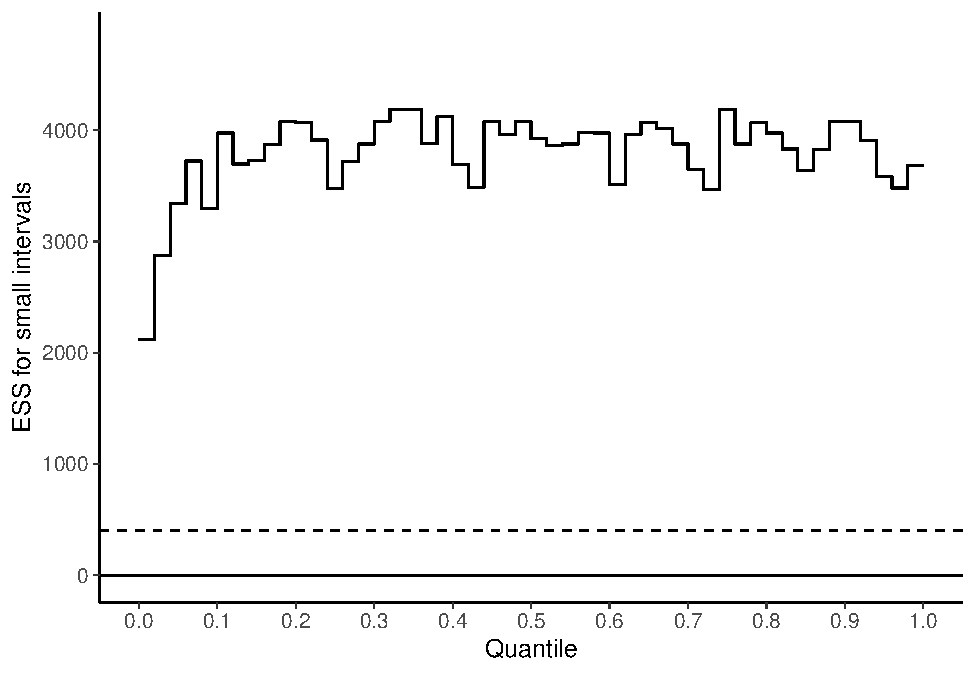
\includegraphics[width=0.6\linewidth]{graphics/local-ess-fit-ncp2-finer-1.pdf}
%   \caption{The local efficiency of small interval probability estimates with more fine resolution for 8 schools model with non-centered parameterization.}
% \end{figure}
% The sampling efficiency for different quantile estimates looks good as
% well.
\begin{figure}[tp]
  \centering
  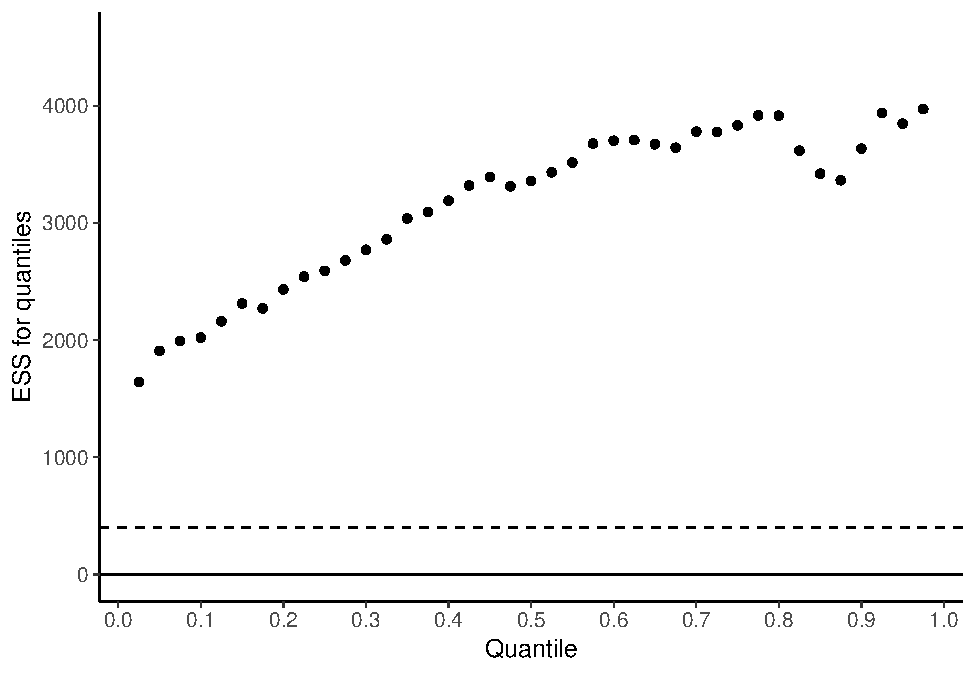
\includegraphics[width=0.6\linewidth]{graphics/quantile-ess-fit-ncp2-1.pdf}
  \caption{The efficiency of quantile estimates for 8 schools model with non-centered parameterization.}
  \label{fig:quantile-ess-fit-ncp2-1}
\end{figure}
Small $\tau$ values are still more difficult to explore, but the
relative efficiency is good.
% We may also check this with a finer resolution:
%
The rank plots of $\tau$ Figure~\ref{fig:hist-fit-ncp2-1} show no
substantial differences between chains.
\begin{figure}[tp]
  \centering
  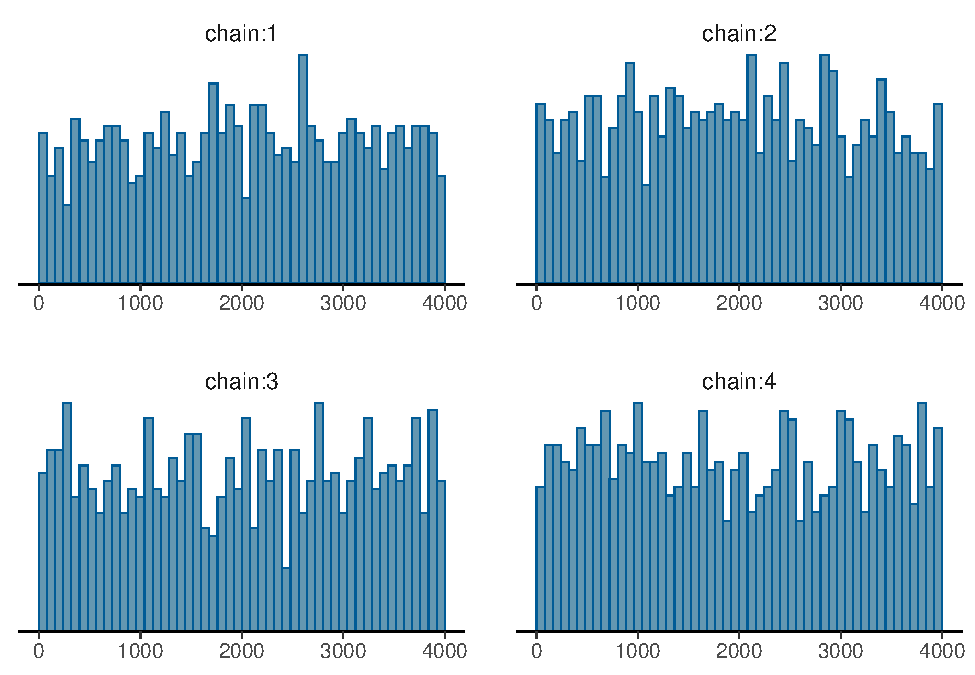
\includegraphics[width=0.6\linewidth]{graphics/hist-fit-ncp2-1.pdf}
  \caption{Rank plots of posterior draws from four chains for 8 schools model with non-centered parameterization.}
  \label{fig:hist-fit-ncp2-1}
\end{figure}

\FloatBarrier

% \hypertarget{references}{%
% \section*{References}\label{references}}
% \addcontentsline{toc}{section}{References}

% \hypertarget{refs}{}

\hypertarget{appendices}{%
\section*{Appendices}\label{appendices}}
\addcontentsline{toc}{section}{Appendices}

% \hypertarget{AppendixA}{%
% \subsection*{Appendix A: Abbreviations}\label{AppendixA}}
% \addcontentsline{toc}{subsection}{Appendix A: Abbreviations}

% The following abbreviations are used throughout the appendices:

% \begin{itemize}
% \tightlist
% \item
%   N = total number of draws
% \item
%   Rhat = classic no-split-Rhat
% \item
%   sRhat = classic split-Rhat
% \item
%   zsRhat = rank-normalized split-Rhat

%   \begin{itemize}
%   \tightlist
%   \item
%     all chains are jointly ranked and z-transformed
%   \item
%     can detect differences in location and trends
%   \end{itemize}
% \item
%   zfsRhat = rank-normalized folded split-Rhat

%   \begin{itemize}
%   \tightlist
%   \item
%     all chains are jointly ``folded'' by computing absolute deviation
%     from median, ranked and z-transformed
%   \item
%     can detect differences in scales
%   \end{itemize}
% \item
%   seff = no-split effective sample size
% \item
%   reff = seff / N
% \item
%   zsseff = rank-normalized split effective sample size

%   \begin{itemize}
%   \tightlist
%   \item
%     estimates the efficiency of mean estimate for rank normalized values
%   \end{itemize}
% \item
%   zsreff = zsseff / N
% \item
%   zfsseff = rank-normalized folded split effective sample size

%   \begin{itemize}
%   \tightlist
%   \item
%     estimates the efficiency of rank normalized \emph{mean} absolute
%     deviation
%   \end{itemize}
% \item
%   zfsreff = zfsseff / N
% \item
%   tailseff = minimum of rank-normalized split effective sample sizes of
%   the 5\% and 95\% quantiles
% \item
%   tailreff = tailseff / N
% \item
%   medsseff = median split effective sample size

%   \begin{itemize}
%   \tightlist
%   \item
%     estimates the efficiency of the median
%   \end{itemize}
% \item
%   medsreff = medsseff / N
% \item
%   madsseff = mad split effective sample size

%   \begin{itemize}
%   \tightlist
%   \item
%     estimates the efficiency of the median absolute deviation
%   \end{itemize}
% \item
%   madsreff = madsseff / N
% \end{itemize}

% \hypertarget{AppendixB}{%
% \subsection*{Appendix B: Examples of rank
% normalization}\label{AppendixB}}
% \addcontentsline{toc}{subsection}{Appendix B: Examples of rank
% normalization}

% We will illustrate the rank normalization with a few examples. First, we
% plot histograms, and empirical cumulative distribution functions (ECDF)
% with respect to the original parameter values (\(\theta\)), scaled ranks
% (ranks divided by the maximum rank), and rank normalized values (z). We
% used scaled ranks to make the plots look similar for different number of
% draws.

% 100 draws from Normal(0, 1):

% \begin{figure}[tp]
%   \centering
%   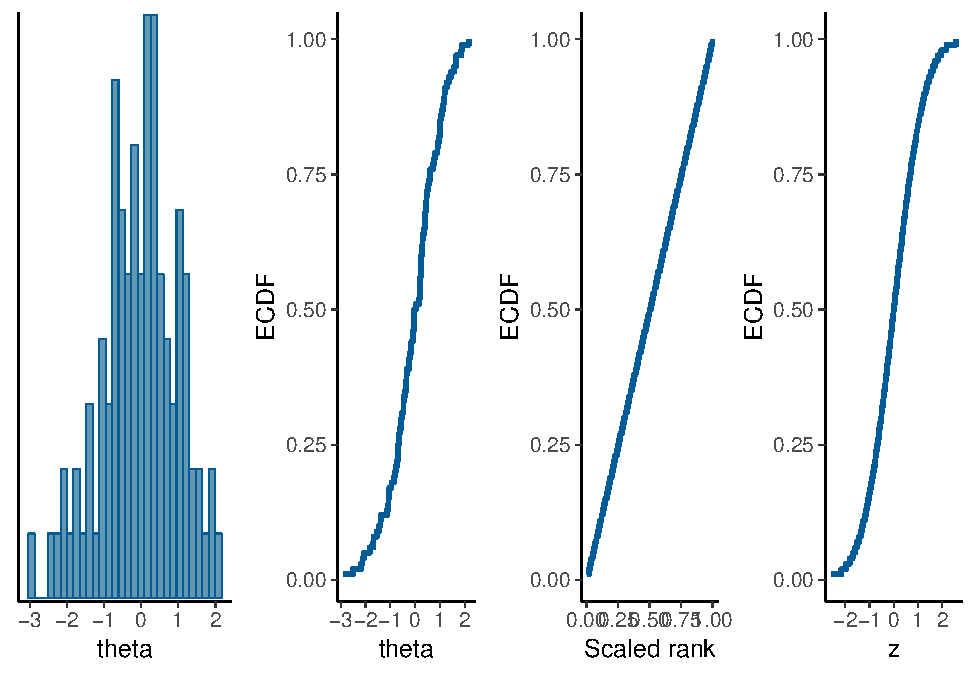
\includegraphics[width=0.6\linewidth]{graphics/ranknorm-normal-1.pdf}
% \end{figure}

% 100 draws from Exponential(1):

% \begin{figure}[tp]
%   \centering
%   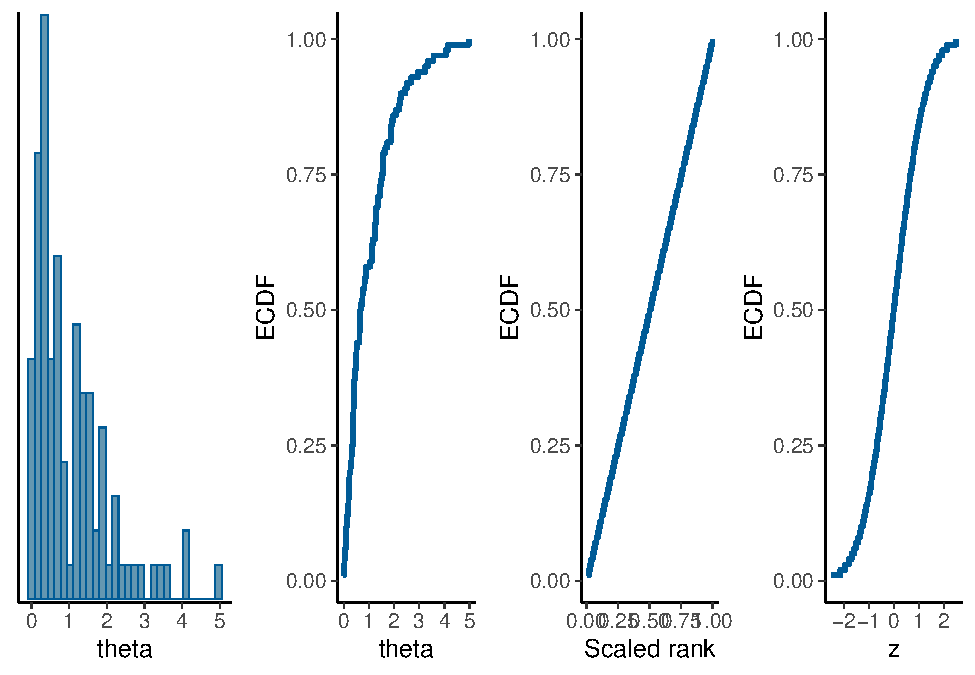
\includegraphics[width=0.6\linewidth]{graphics/ranknorm-exp-1.pdf}
% \end{figure}

% 100 draws from Cauchy(0, 1):

% \begin{figure}[tp]
%   \centering
%   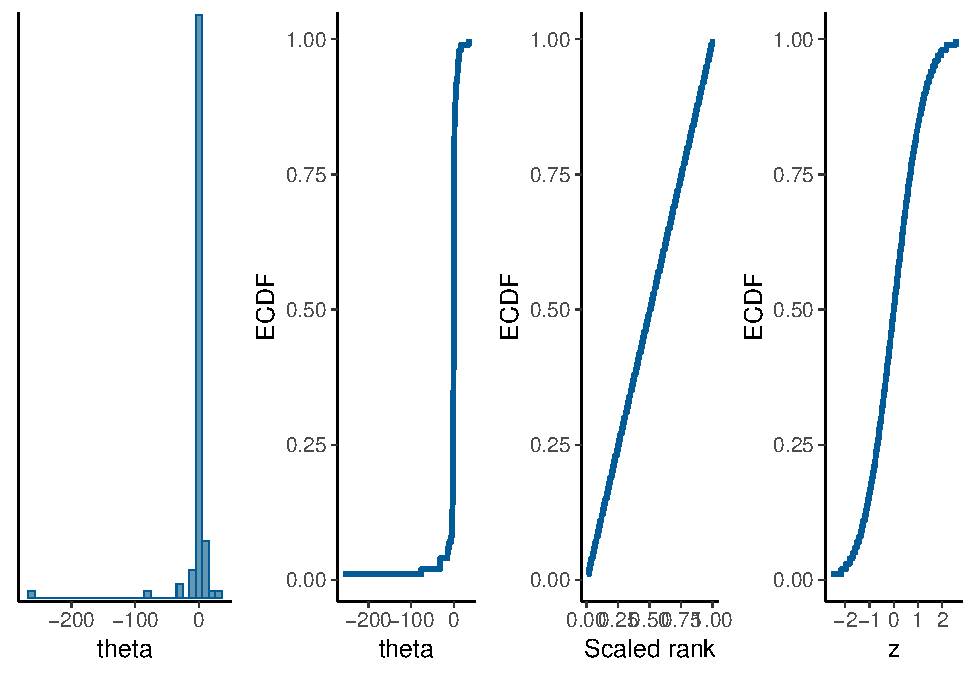
\includegraphics[width=0.6\linewidth]{graphics/ranknorm-cauchy-1.pdf}
% \end{figure}

% In the above plots, the ECDF with respect to scaled rank and rank
% normalized \(z\)-values look exactly the same for all distributions. In
% \emph{Split}-\(\widehat{R}\) and effective sample size computations, we
% rank all draws jointly, but then compare ranks and ECDF of individual
% split chains. To illustrate the variation between chains, we draw 8
% batches of 100 draws each from Normal(0, 1):

% \begin{figure}[tp]
%   \centering
%   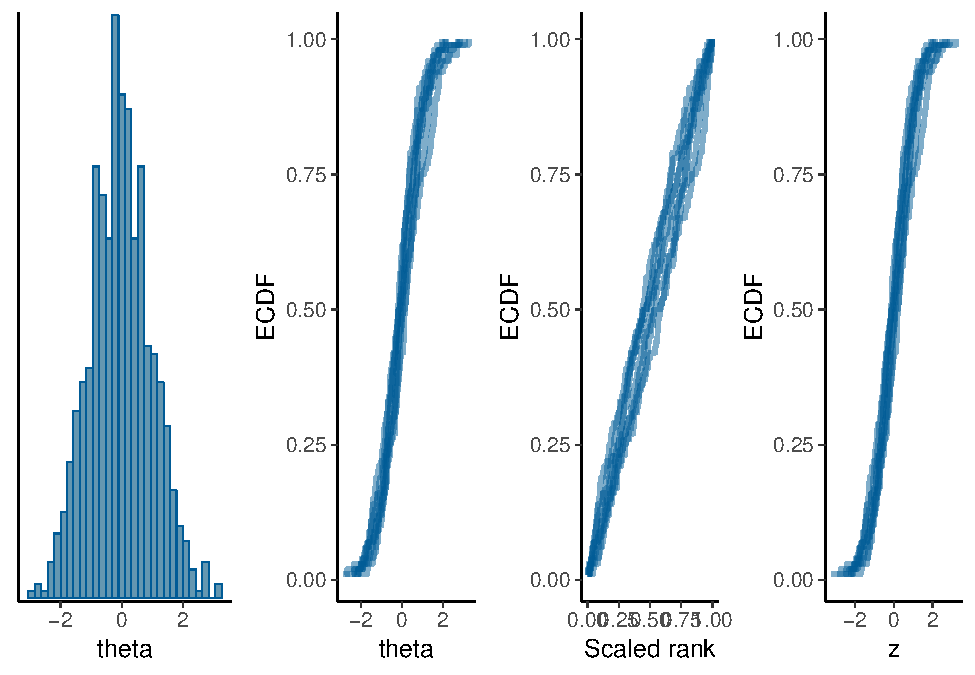
\includegraphics[width=0.6\linewidth]{graphics/ranknorm-normal2-1.pdf}
% \end{figure}

% The variation in ECDF due to the variation ranks is now visible also in
% scaled ranks and rank normalized \(z\)-values from different batches
% (chains).

% The benefit of rank normalization is more obvious for non-normal
% distribution such as Cauchy:

% \begin{figure}[tp]
%   \centering
%   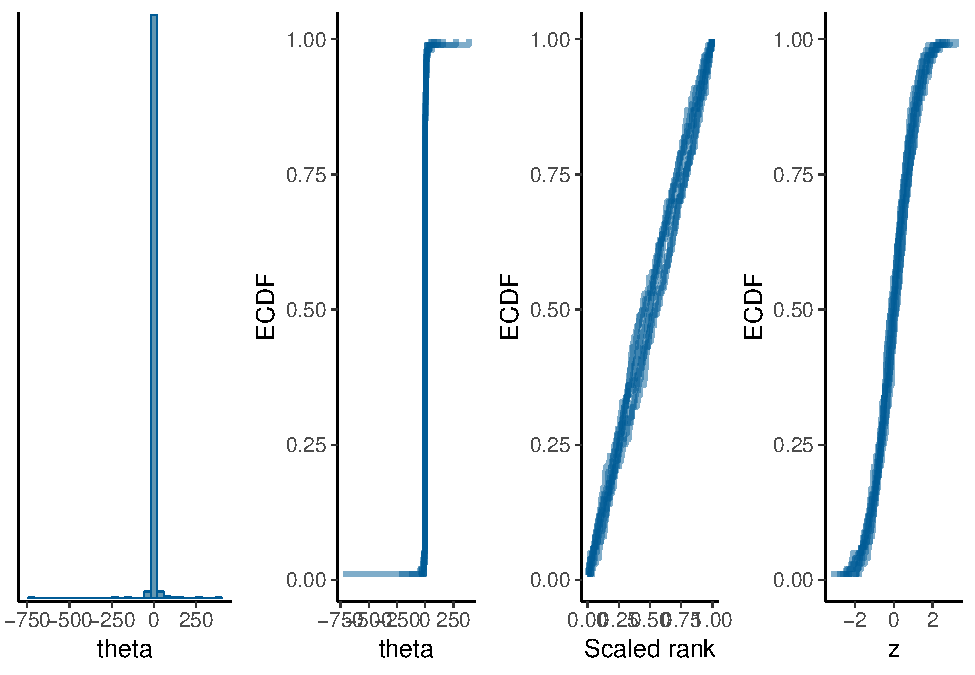
\includegraphics[width=0.6\linewidth]{graphics/ranknorm-cauchy2-1.pdf}
% \end{figure}

% Rank normalization makes the subsequent computations well defined and
% invariant under bijective transformations. This means that we get the
% same results, for example, if we use unconstrained or constrained
% parameterisations in a model.

% \hypertarget{AppendixC}{%
% \subsection*{Appendix C: Variance of the cumulative distribution
% function}\label{AppendixC}}
% \addcontentsline{toc}{subsection}{Appendix C: Variance of the cumulative
% distribution function}

% In Section 3, we had defined the empirical CDF (ECDF) for any
% \(\theta_\alpha\) as

% \[
% p(\theta \leq \theta_\alpha) \approx \bar{I}_\alpha = \frac{1}{S}\sum_{s=1}^S
% I(\theta^{(s)} \leq\theta_\alpha),
% \]

% For independent draws, \(\bar{I}_\alpha\) has a
% \({\rm Beta}(\bar{I}_\alpha+1, S - \bar{I}_\alpha + 1)\) distribution.
% Thus we can easily examine the variation of the ECDF for any
% \(\theta_\alpha\) value from a single chain. If \(\bar{I}_\alpha\) is
% not very close to \(1\) or \(S\) and \(S\) is large, we can use the
% variance of Beta distribution

% \[
% {\rm Var}[p(\theta \leq \theta_\alpha)] =
% \frac{(\bar{I}_\alpha+1)*(S-\bar{I}_\alpha+1)}{(S+2)^2(S+3)}.
% \] We illustrate uncertainty intervals of the Beta distribution and
% normal approximation of ECDF for 100 draws from Normal(0, 1):

% \begin{figure}[tp]
%   \centering
%   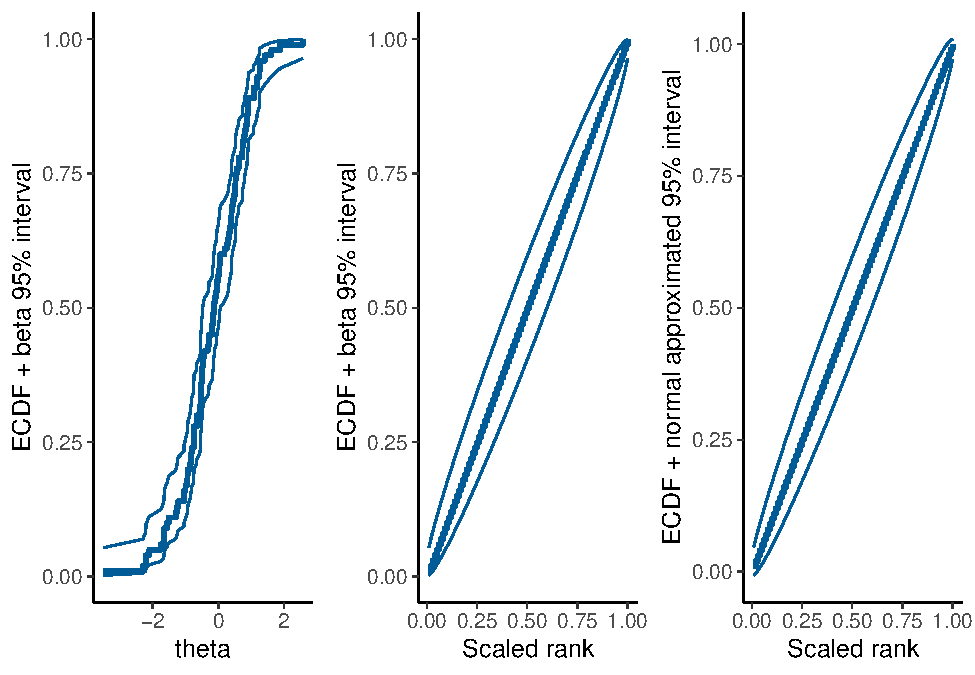
\includegraphics[width=0.6\linewidth]{graphics/ranknorm-beta-1.pdf}
% \end{figure}

% Uncertainty intervals of ECDF for draws from Cauchy(0, 1) illustrate
% again the improved visual clarity in plotting when using scaled ranks:

% \begin{figure}[tp]
%   \centering
%   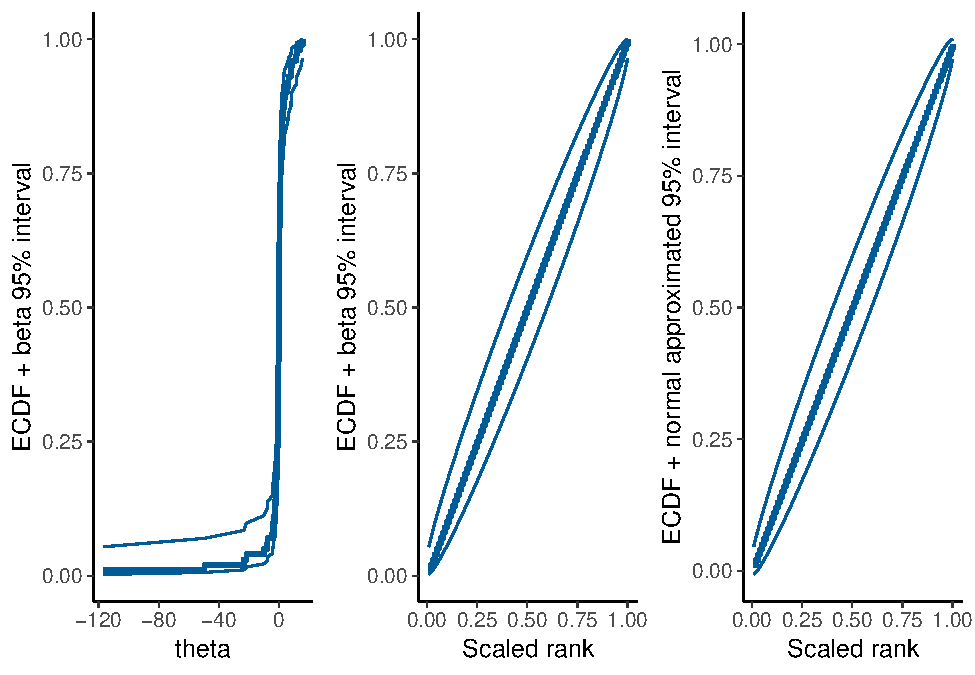
\includegraphics[width=0.6\linewidth]{graphics/ranknorm-cauchy3-1.pdf}
% \end{figure}

% The above plots illustrate that the normal approximation is accurate for
% practical purposes in MCMC diagnostics.

% \FloatBarrier

\hypertarget{AppendixD}{%
\subsection*{Appendix D: Normal distributions with additional trend,
shift or scaling}\label{AppendixD}}
\addcontentsline{toc}{subsection}{Appendix D: Normal distributions with
additional trend, shift or scaling}

This part focuses on diagnostics for

\begin{itemize}
\tightlist
\item
  all chains having a trend and a similar marginal distribution
\item
  one of the chains having a different mean
\item
  one of the chains having a lower marginal variance
\end{itemize}

To simplify, in this part, independent draws are used as a proxy for
very efficient MCMC sampling. First, we sample draws from a
standard-normal distribution. We will discuss the behavior for
non-normal distributions later. See
\protect\hyperlink{AppendixA}{Appendix A} for the abbreviations used.

\hypertarget{adding-the-same-trend-to-all-chains}{%
\subsubsection*{Adding the same trend to all
chains}\label{adding-the-same-trend-to-all-chains}}
\addcontentsline{toc}{subsubsection}{Adding the same trend to all
chains}

All chains are from the same Normal(0, 1) distribution plus a linear
trend added to all chains:

If we don't split chains, Rhat misses the trends if all chains still
have a similar marginal distribution.

\begin{figure}[tp]
  \centering
  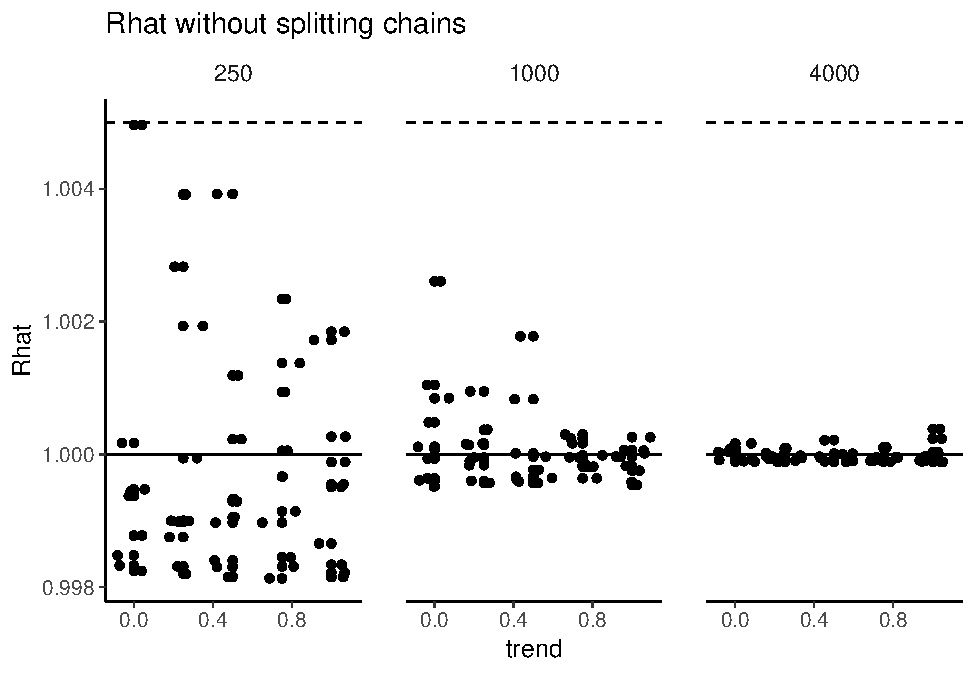
\includegraphics[width=0.6\linewidth]{graphics/rhat-same-trend-1.pdf}
\end{figure}

Split-Rhat can detect trends, even if the marginals of the chains are
similar.

\begin{figure}[tp]
  \centering
  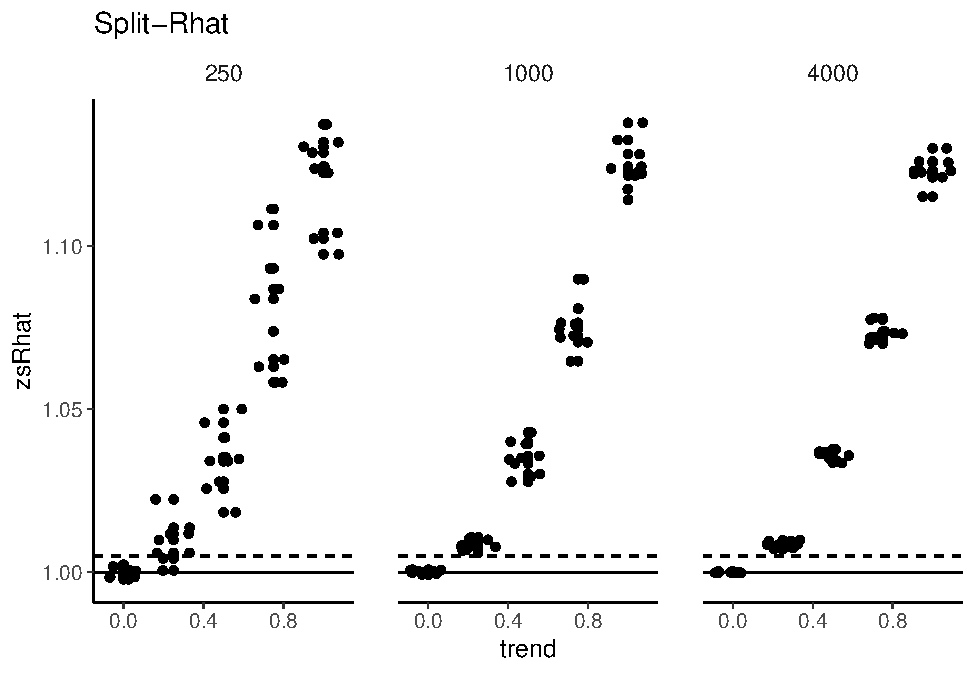
\includegraphics[width=0.6\linewidth]{graphics/zsrhat-same-trend-1.pdf}
\end{figure}

\textbf{Result:} Split-Rhat is useful for detecting non-stationarity
(i.e., trends) in the chains. If we use a threshold of \(1.01\), we can
detect trends which account for 2\% or more of the total marginal
variance. If we use a threshold of \(1.1\), we detect trends which
account for 30\% or more of the total marginal variance.

The effective sample size is based on split Rhat and within-chain
autocorrelation. We plot the relative efficiency
\(R_{\rm eff}=S_{\rm eff}/S\) for easier comparison between different
values of \(S\). In the plot below, dashed lines indicate the threshold
at which we would consider the effective sample size to be sufficient
(i.e., \(S_{\rm eff} > 400\)). Since we plot the relative efficiency
instead of the effective sample size itself, this threshold is divided
by \(S\), which we compute here as the number of iterations per chain
(variable \texttt{iter}) times the number of chains (\(4\)).

\begin{figure}[tp]
  \centering
  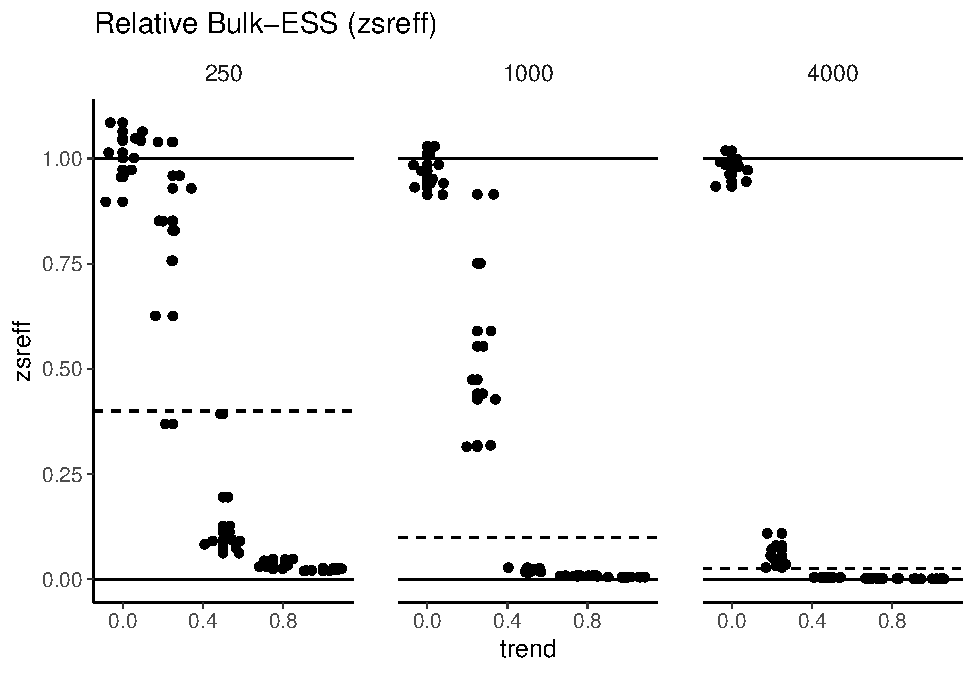
\includegraphics[width=0.6\linewidth]{graphics/zsreff-same-trend-1.pdf}
\end{figure}

\textbf{Result:} Split-Rhat is more sensitive to trends for small sample
sizes, but effective sample size becomes more sensitive for larger
samples sizes (as autocorrelations can be estimated more accurately).

\textbf{Advice:} If in doubt, run longer chains for more accurate
convergence diagnostics.

\hypertarget{shifting-one-chain}{%
\subsubsection*{Shifting one chain}\label{shifting-one-chain}}
\addcontentsline{toc}{subsubsection}{Shifting one chain}

Next we investigate the sensitivity to detect if one of the chains has
not converged to the same distribution as the others, but has a
different mean.

\begin{figure}[tp]
  \centering
  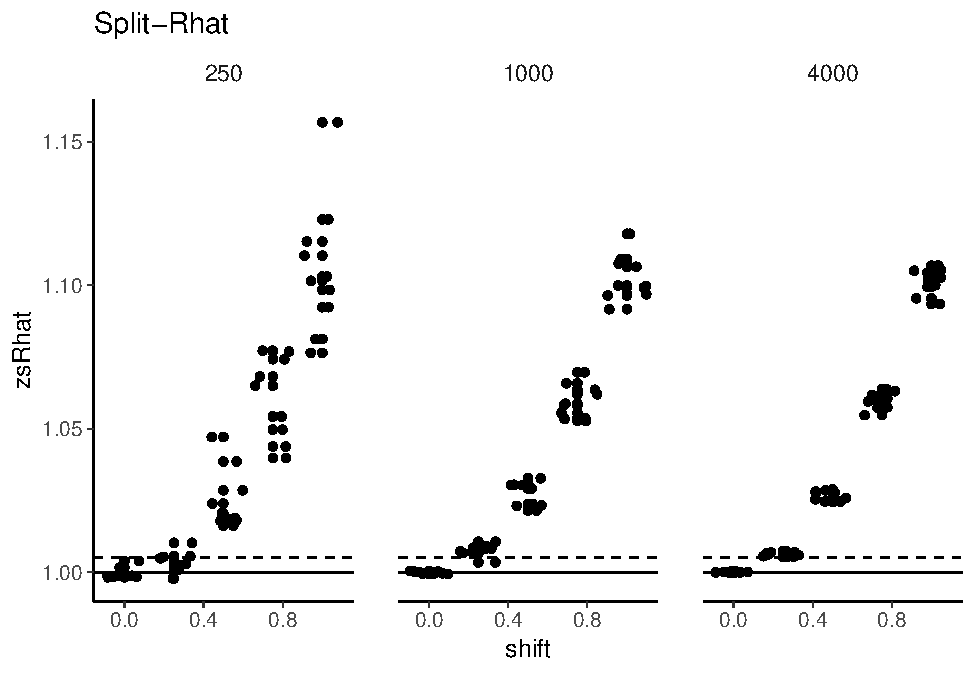
\includegraphics[width=0.6\linewidth]{graphics/zsrhat-shifted-chain-1.pdf}
\end{figure}

\textbf{Result:} If we use a threshold of \(1.01\), we can detect shifts
with a magnitude of one third or more of the marginal standard
deviation. If we use a threshold of \(1.1\), we detect shifts with a
magnitude equal to or larger than the marginal standard deviation.

\begin{figure}[tp]
  \centering
  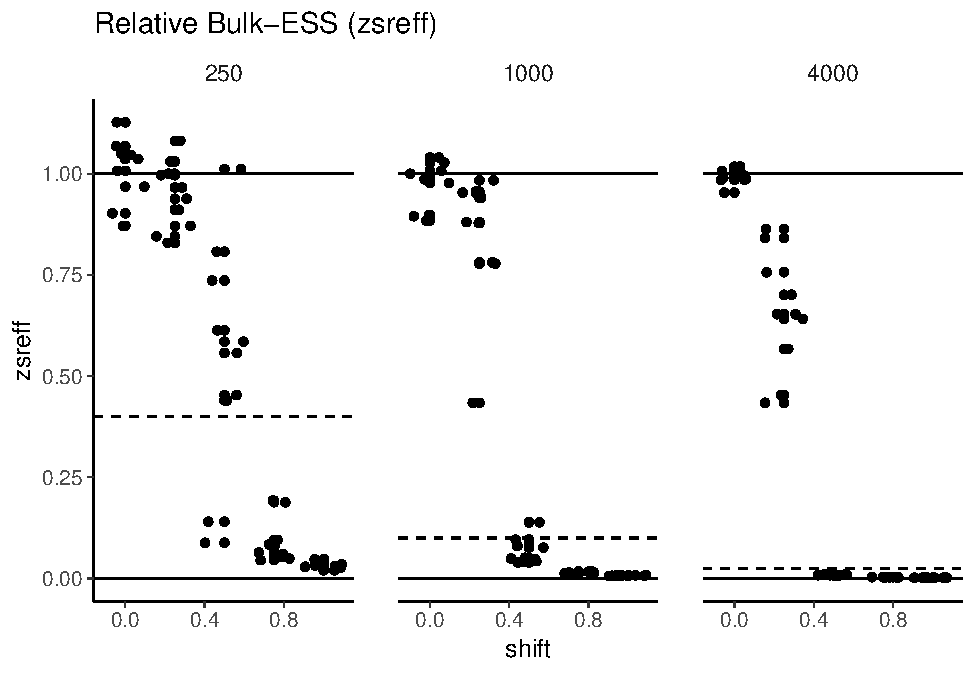
\includegraphics[width=0.6\linewidth]{graphics/zsreff-shifted-chain-1.pdf}
\end{figure}

\textbf{Result:} The effective sample size is not as sensitive, but a
shift with a magnitude of half the marginal standard deviation or more
will lead to very low relative efficiency when the total number of draws
increases.

Rank plots can be used to visualize differences between chains. Here, we
show rank plots for the case of 4 chains, 250 draws per chain, and a
shift of 0.5.

\begin{figure}[tp]
  \centering
  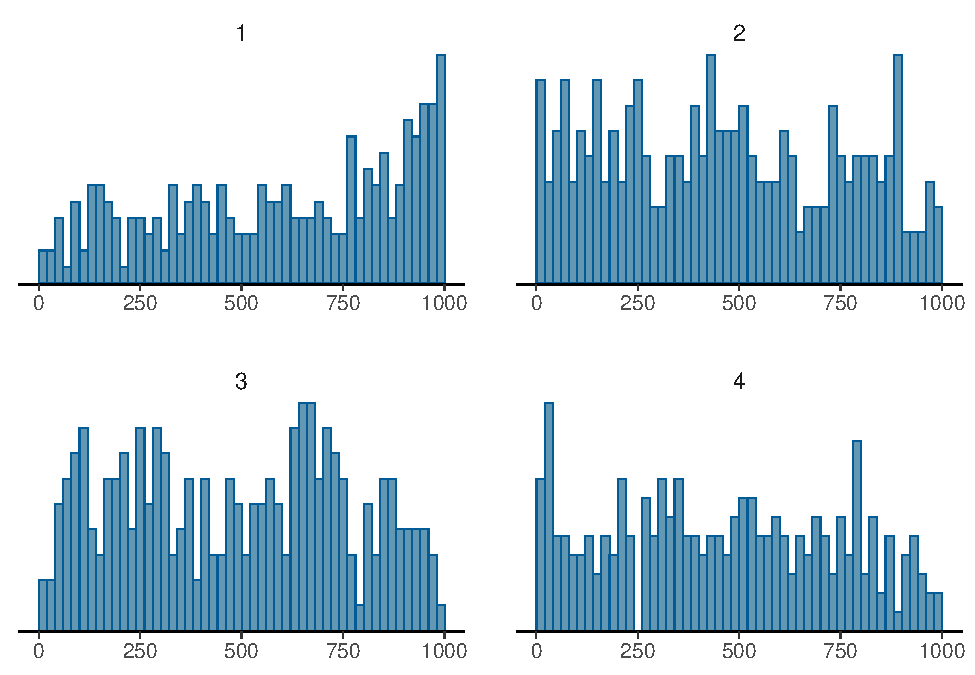
\includegraphics[width=0.6\linewidth]{graphics/hist-shifted-chain-1.pdf}
\end{figure}

Although, Rhat was less than \(1.05\) for this situation, the rank plots
clearly show that the first chains behaves differently.

\hypertarget{scaling-one-chain}{%
\subsubsection*{Scaling one chain}\label{scaling-one-chain}}
\addcontentsline{toc}{subsubsection}{Scaling one chain}

Next, we investigate the sensitivity to detect if one of the chains has
not converged to the same distribution as the others, but has lower
marginal variance.

We first look at the Rhat estimates:

\begin{figure}[tp]
  \centering
  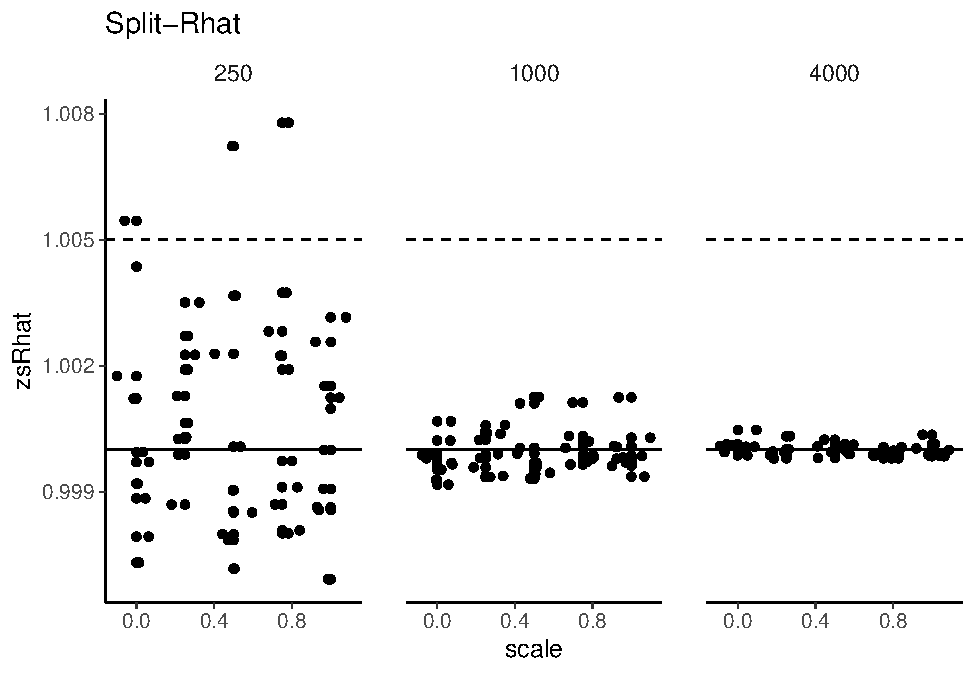
\includegraphics[width=0.6\linewidth]{graphics/zsrhat-scaled-chain-1.pdf}
\end{figure}

\textbf{Result:} Split-Rhat is not able to detect scale differences
between chains.

\begin{figure}[tp]
  \centering
  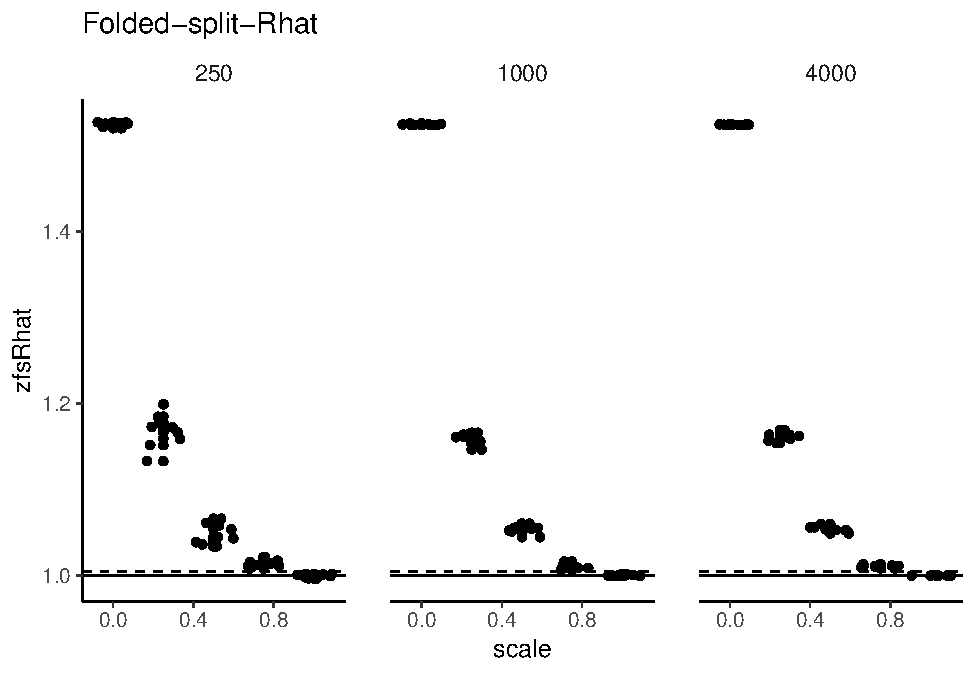
\includegraphics[width=0.6\linewidth]{graphics/zfsrhat-scaled-chain-1.pdf}
\end{figure}

\textbf{Result:} Folded-Split-Rhat focuses on scales and detects scale
differences.

\textbf{Result:} If we use a threshold of \(1.01\), we can detect a
chain with scale less than \(3/4\) of the standard deviation of the
others. If we use threshold of \(1.1\), we detect a chain with standard
deviation less than \(1/4\) of the standard deviation of the others.

Next, we look at the effective sample size estimates:

\begin{figure}[tp]
  \centering
  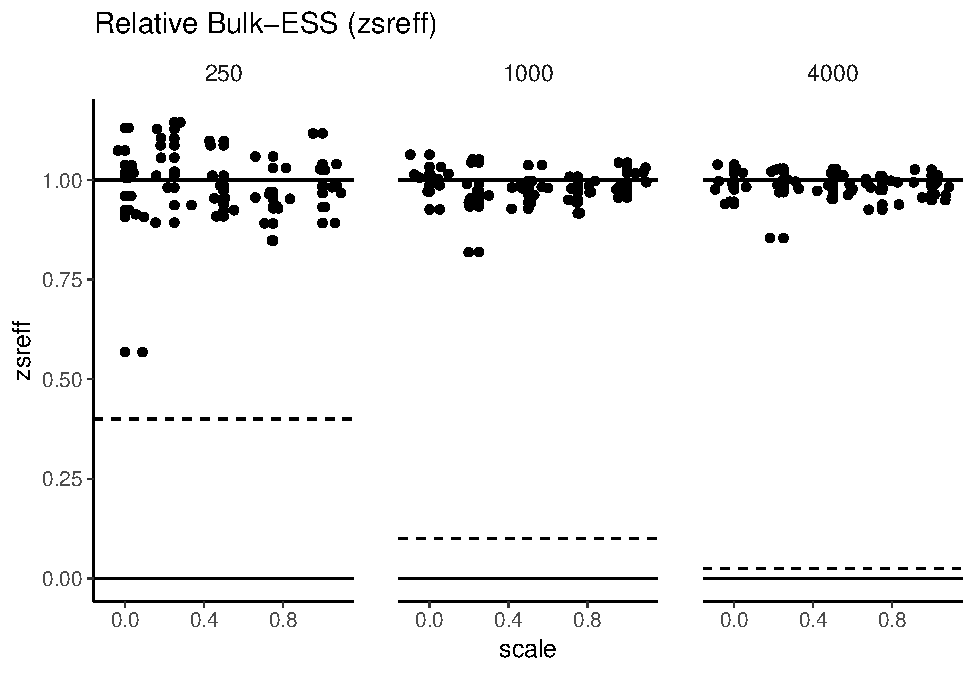
\includegraphics[width=0.6\linewidth]{graphics/zsreff-scaled-chain-1.pdf}
\end{figure}

\textbf{Result:} The bulk effective sample size of the mean does not see
a problem as it focuses on location differences between chains.

Rank plots can be used to visualize differences between chains. Here, we
show rank plots for the case of 4 chains, 250 draws per chain, and with
one chain having a standard deviation of 0.75 as opposed to a standard
deviation of 1 for the other chains.

\begin{figure}[tp]
  \centering
  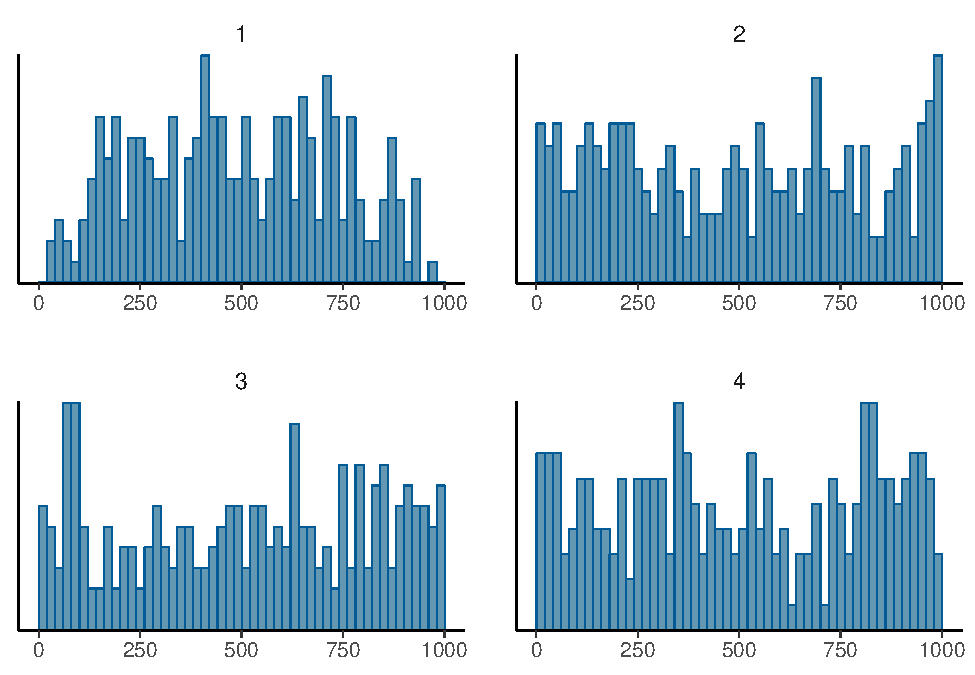
\includegraphics[width=0.6\linewidth]{graphics/hist-scaled-chain-1.pdf}
\end{figure}

Although folded Rhat is \(1.06\), the rank plots clearly show that the
first chains behaves differently.

\hypertarget{AppendixE}{%
\subsection*{Appendix E: Cauchy: A distribution with infinite mean and
variance}\label{AppendixE}}
\addcontentsline{toc}{subsection}{Appendix E: Cauchy: A distribution
with infinite mean and variance}

The classic split-Rhat is based on calculating within and between chain
variances. If the marginal distribution of a chain is such that the
variance is not defined (i.e.~infinite), the classic split-Rhat is not
well justified. In this section, we will use the Cauchy distribution as
an example of such distribution. Also in cases where mean and variance
are finite, the distribution can be far from Gaussian. Especially
distributions with very long tails cause instability for variance and
autocorrelation estimates. To alleviate these problems we will use
Split-Rhat for rank-normalized draws.

% The following Cauchy models are from Michael Betancourt's case study
% \href{https://betanalpha.github.io/assets/case_studies/fitting_the_cauchy.html}{Fitting
% The Cauchy Distribution}

\hypertarget{nominal-parameterization-of-cauchy-1}{%
\subsubsection*{Nominal parameterization of
Cauchy}\label{nominal-parameterization-of-cauchy-1}}
\addcontentsline{toc}{subsubsection}{Nominal parameterization of Cauchy}

We already looked at the nominal Cauchy model with direct
parameterization in the main text, but for completeness, we take a
closer look using different variants of the diagnostics.

\begin{verbatim}
parameters {
  vector[50] x;
}

model {
  x ~ cauchy(0, 1);
}

generated quantities {
  real I = fabs(x[1]) < 1 ? 1 : 0;
}
\end{verbatim}

\hypertarget{default-stan-options-1}{%
\paragraph{Default Stan options}\label{default-stan-options-1}}
\addcontentsline{toc}{paragraph}{Default Stan options}

Run the nominal model:

Treedepth exceedence and Bayesian Fraction of Missing Information are
dynamic HMC specific diagnostics \citep{betancourt2017conceptual}. We
get warnings about very large number of transitions after warmup that
exceeded the maximum treedepth, which is likely due to very long tails
of the Cauchy distribution. All chains have low estimated Bayesian
fraction of missing information also indicating slow mixing.

Trace plots for the first parameter look wild with occasional large
values:

\begin{figure}[tp]
  \centering
  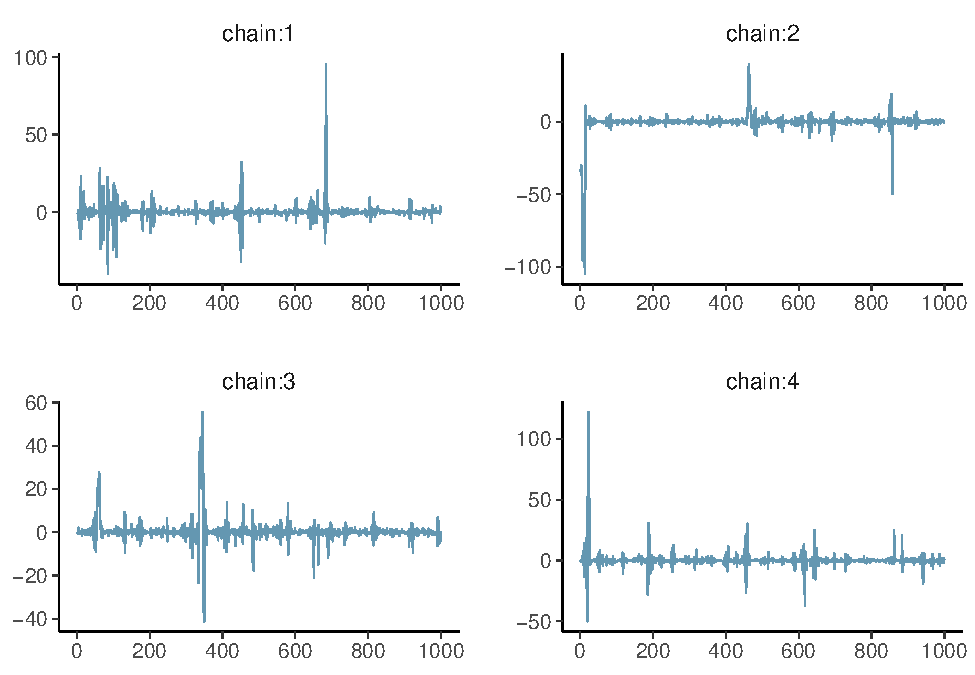
\includegraphics[width=0.6\linewidth]{graphics/trace-fit-nom-1.pdf}
\end{figure}

Let's check Rhat and ESS diagnostics.

\begin{figure}[tp]
  \centering
  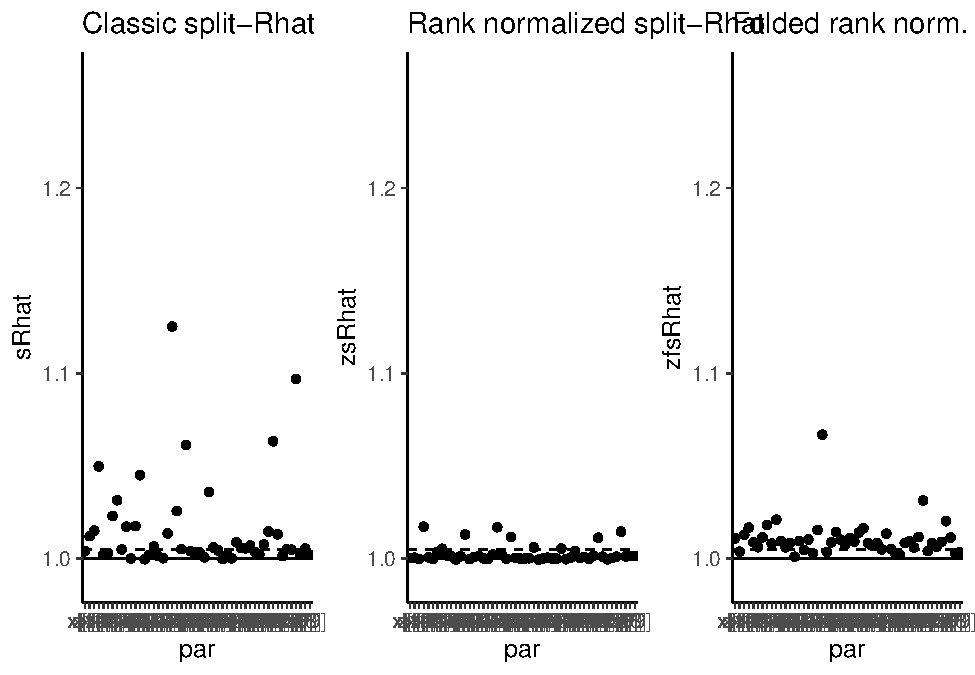
\includegraphics[width=0.6\linewidth]{graphics/rhat-fit-nom-1.pdf}
\end{figure}

For one parameter, Rhats exceed the classic threshold of 1.1. Depending
on the Rhat estimate, a few others also exceed the threshold of 1.01.
The rank normalized split-Rhat has several values over 1.01. Please note
that the classic split-Rhat is not well defined in this example, because
mean and variance of the Cauchy distribution are not finite.

\begin{figure}[tp]
  \centering
  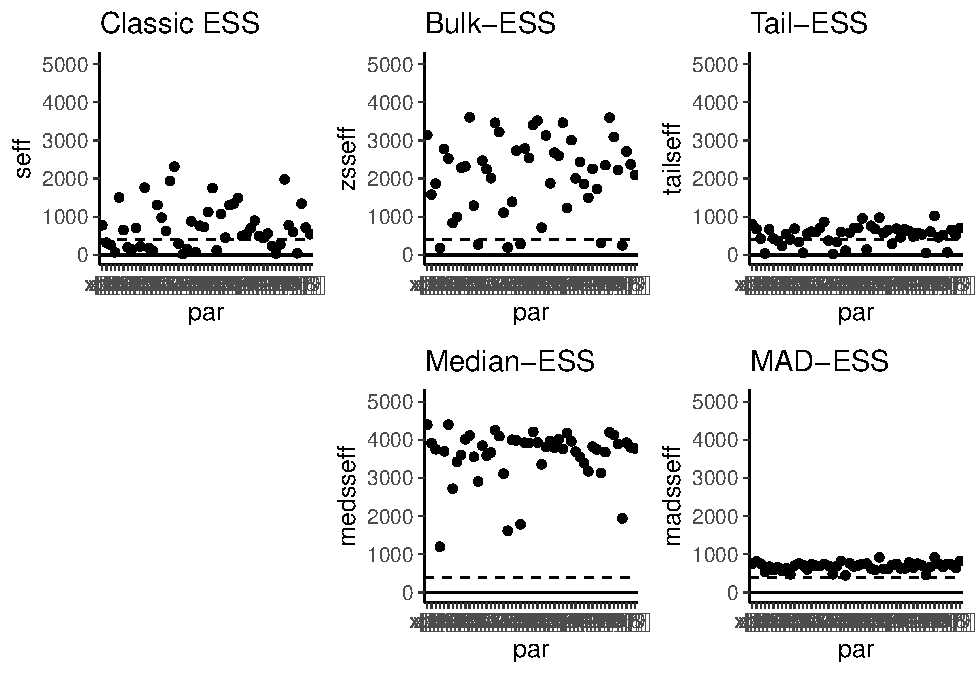
\includegraphics[width=0.6\linewidth]{graphics/ess-fit-nom-1.pdf}
\end{figure}

Both classic and new effective sample size estimates have several very
small values, and so the overall sample shouldn't be trusted.

\textbf{Result:} Effective sample size is more sensitive than
(rank-normalized) split-Rhat to detect problems of slow mixing.

We also check the log posterior value \texttt{lp\_\_} and find out that
the effective sample size is worryingly low.

\begin{verbatim}
lp__: Bulk-ESS =  117
\end{verbatim}

\begin{verbatim}
lp__: Tail-ESS =  323
\end{verbatim}

We can further analyze potential problems using local effective sample
size and rank plots. We examine x{[}36{]}, which has the smallest
tail-ESS of 117.

We examine the sampling efficiency in different parts of the posterior
by computing the effective sample size for small interval probability
estimates (see \protect\hyperlink{small_interval_S_eff}{Section
Efficiency for small interval probability estimates}). Each interval
contains \(1/k\) of the draws (e.g., with \(k=20\)). The small interval
efficiency measures mixing of an indicator function which indicates when
the values are inside the specific small interval. This gives us a local
efficiency measure which does not depend on the shape of the
distribution.

\begin{figure}[tp]
  \centering
  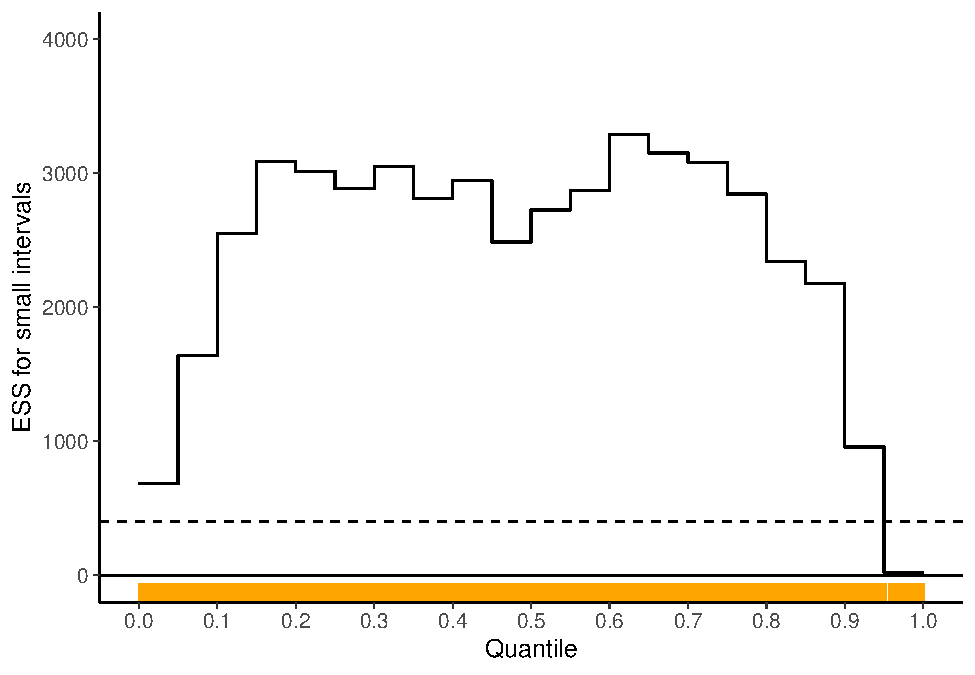
\includegraphics[width=0.6\linewidth]{graphics/local-ess-fit-nom-2-1.pdf}
\end{figure}

We see that the efficiency is worryingly low in the tails (which is
caused by slow mixing in long tails of Cauchy). Orange ticks show draws
that exceeded the maximum treedepth.

An alternative way to examine the effective sample size in different
parts of the posterior is to compute effective sample size for quantiles
(see \protect\hyperlink{quantile_S_eff}{Section Efficiency for
quantiles}). Each interval has a specified proportion of draws, and the
efficiency measures mixing of an indicator function's results which
indicate when the values are inside the specific interval.

\begin{figure}[tp]
  \centering
  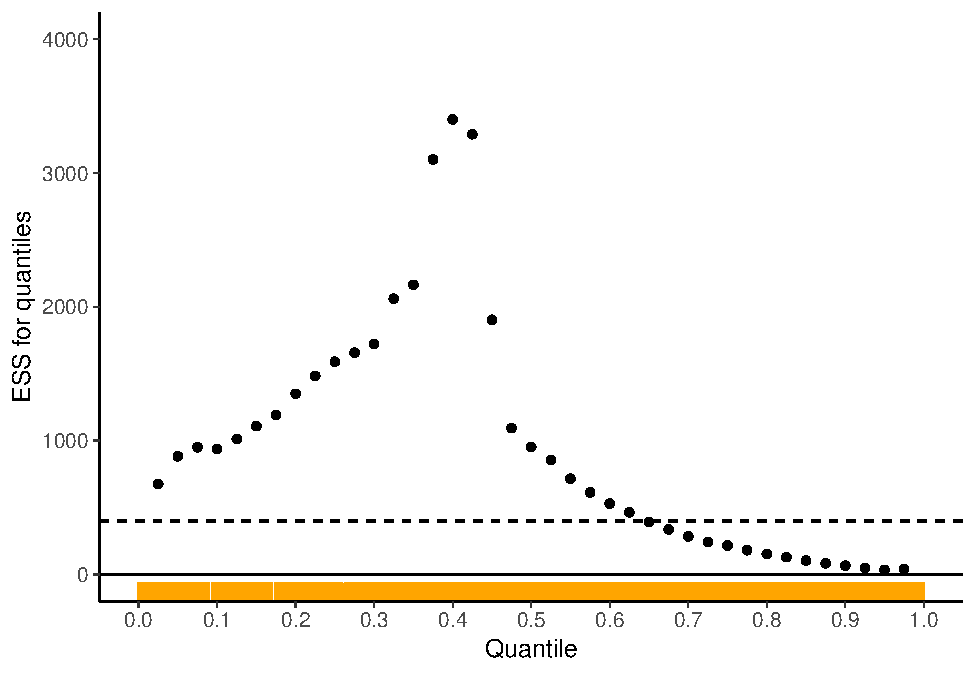
\includegraphics[width=0.6\linewidth]{graphics/quantile-ess-fit-nom-2-1.pdf}
\end{figure}

We see that the efficiency is worryingly low in the tails (which is
caused by slow mixing in long tails of Cauchy). Orange ticks show draws
that exceeded the maximum treedepth.

We can further analyze potential problems using rank plots, from which
we clearly see differences between chains.

\begin{figure}[tp]
  \centering
  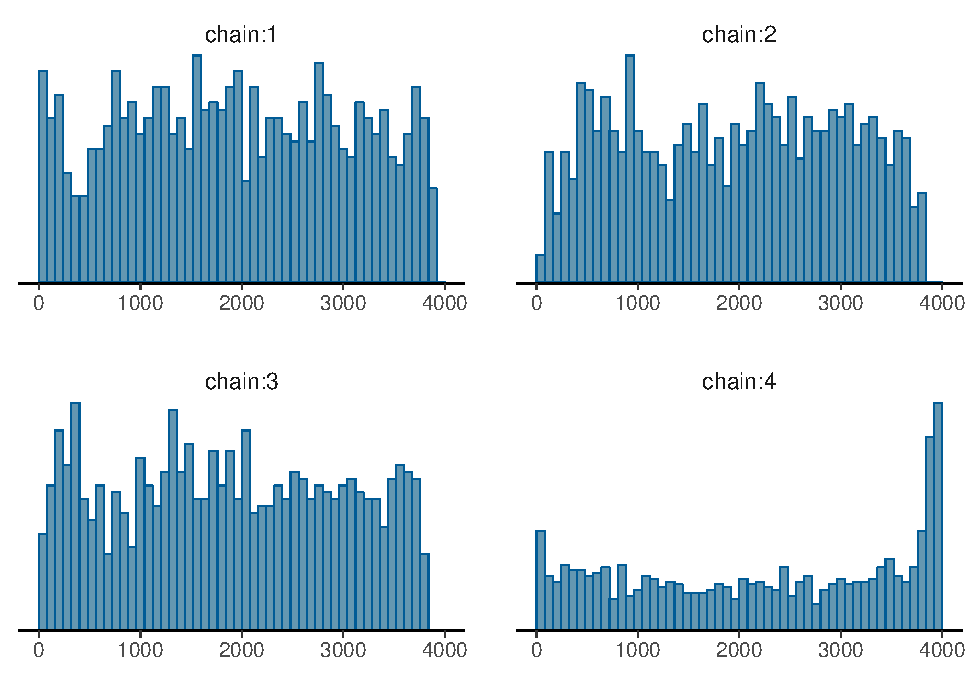
\includegraphics[width=0.6\linewidth]{graphics/hist-fit-nom-2-1.pdf}
\end{figure}

\hypertarget{default-stan-options-increased-maximum-treedepth}{%
\paragraph{Default Stan options + increased maximum
treedepth}\label{default-stan-options-increased-maximum-treedepth}}
\addcontentsline{toc}{paragraph}{Default Stan options + increased
maximum treedepth}

We can try to improve the performance by increasing
\texttt{max\_treedepth} to \(20\):

Trace plots for the first parameter still look wild with occasional
large values.

\begin{figure}[tp]
  \centering
  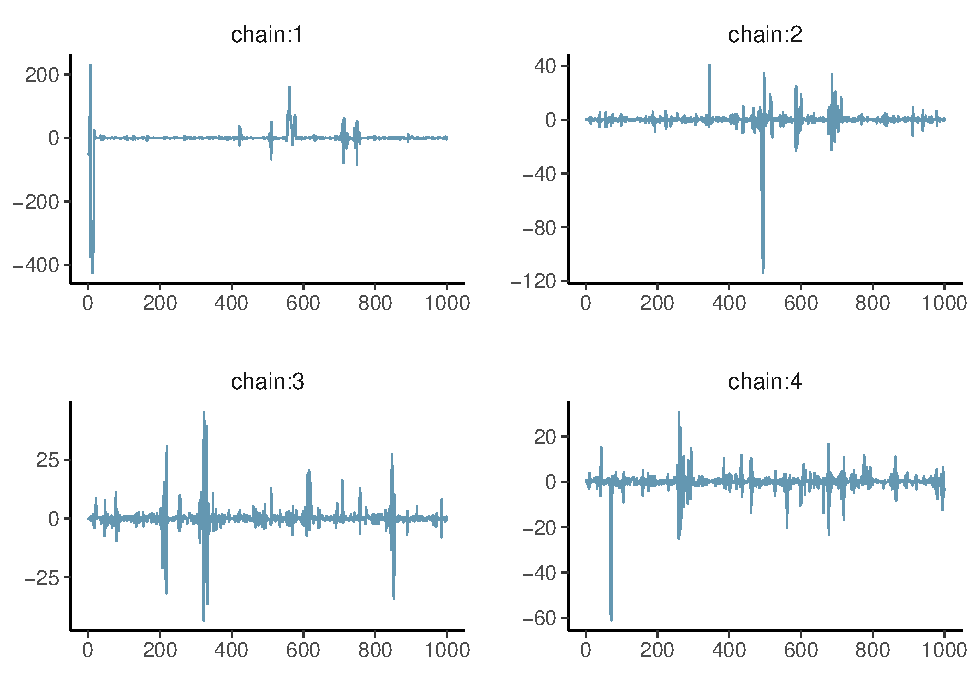
\includegraphics[width=0.6\linewidth]{graphics/trace-fit-nom-td20-1.pdf}
\end{figure}

We check the diagnostics for all \(x\).

\begin{figure}[tp]
  \centering
  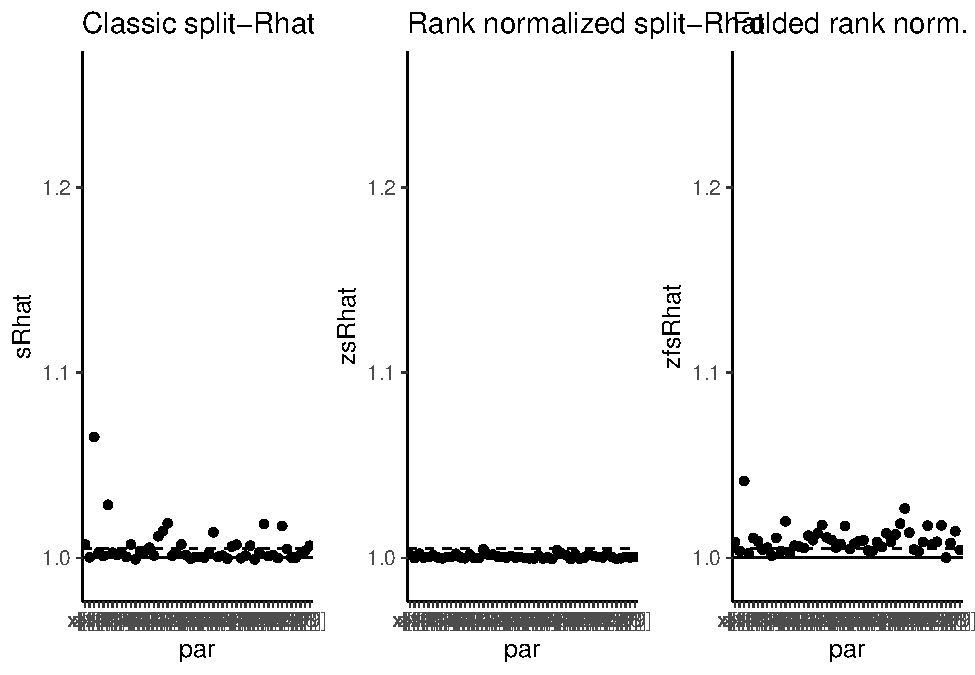
\includegraphics[width=0.6\linewidth]{graphics/rhat-fit-nom-td20-1.pdf}
\end{figure}

All Rhats are below \(1.1\), but many are over \(1.01\). Classic
split-Rhat has more variation than the rank normalized Rhat (note that
the former is not well defined). The folded rank normalized Rhat shows
that there is still more variation in the scale than in the location
between different chains.

\begin{figure}[tp]
  \centering
  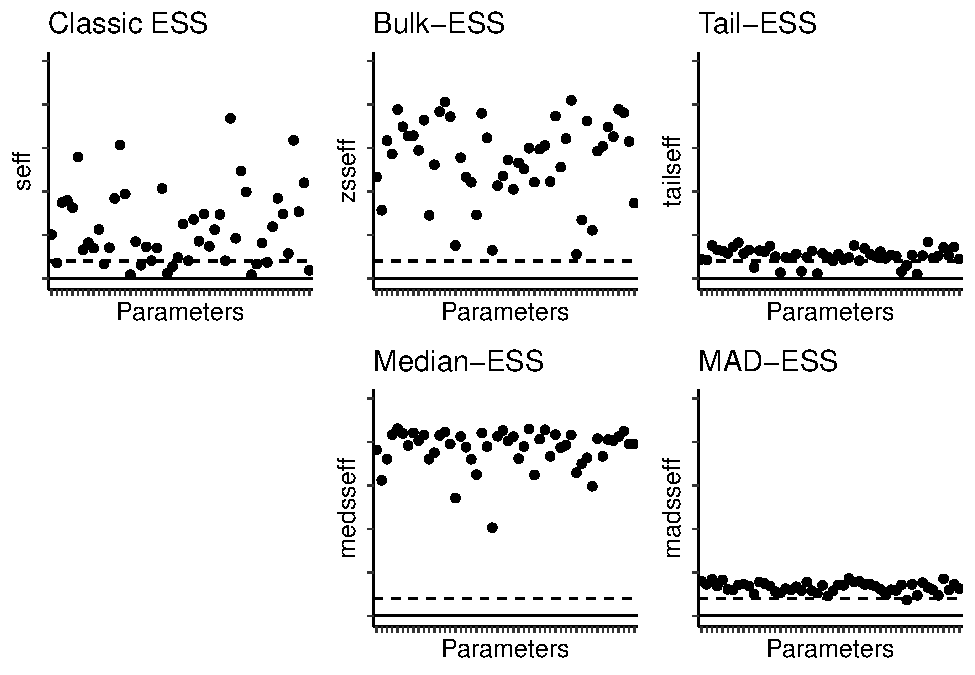
\includegraphics[width=0.6\linewidth]{graphics/ess-fit-nom-td20-1.pdf}
\end{figure}

Some classic effective sample sizes are very small. If we wouldn't
realize that the variance is infinite, we might try to run longer
chains, but in case of an infinite variance, zero relative efficiency
(ESS/S) is the truth and longer chains won't help with that. However
other quantities can be well defined, and that's why it is useful to
also look at the rank normalized version as a generic transformation to
achieve finite mean and variance. The smallest bulk-ESS is less than
1000, which is not that bad. The smallest median-ESS is larger than
2500, that is we are able to estimate the median efficiently. However,
many tail-ESS's are less than 400 indicating problems for estimating the
scale of the posterior.

\textbf{Result:} The rank normalized effective sample size is more
stable than classic effective sample size, which is not well defined for
the Cauchy distribution.

\textbf{Result:} It is useful to look at both bulk- and tail-ESS.

We check also \texttt{lp\_\_}. Although increasing
\texttt{max\_treedepth} improved bulk-ESS of \texttt{x}, the efficiency
for \texttt{lp\_\_} didn't change.

\begin{verbatim}
lp__: Bulk-ESS = 240
\end{verbatim}

\begin{verbatim}
lp__: Tail-ESS = 587
\end{verbatim}

We examine the sampling efficiency in different parts of the posterior
by computing the effective sample size for small interval probability
estimates.

\begin{figure}[tp]
  \centering
  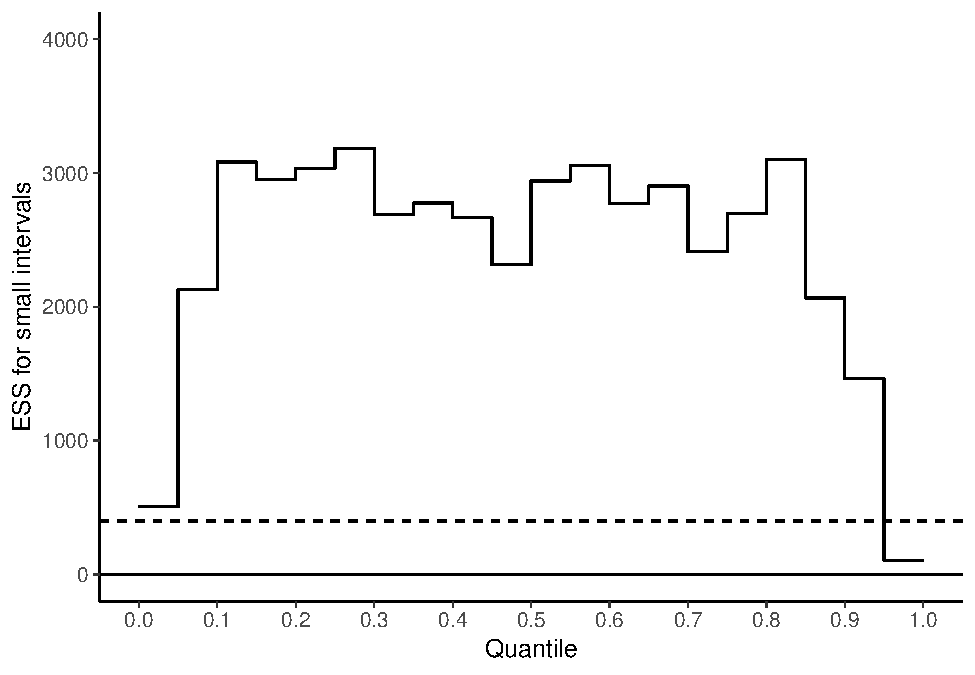
\includegraphics[width=0.6\linewidth]{graphics/local-ess-fit-nom-td20-1.pdf}
\end{figure}

It seems that increasing \texttt{max\_treedepth} has not much improved
the efficiency in the tails. We also examine the effective sample size
of different quantile estimates.

\begin{figure}[tp]
  \centering
  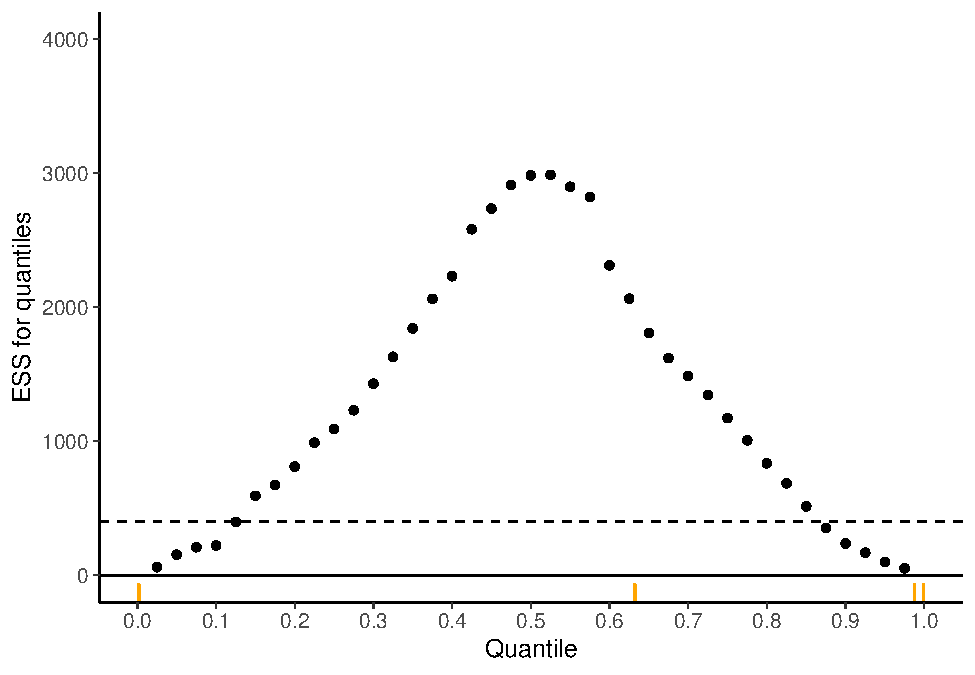
\includegraphics[width=0.6\linewidth]{graphics/quantile-ess-fit-nom-td20-1.pdf}
\end{figure}

The rank plot visualisation of x{[}11{]}, which has the smallest
tail-ESS of NaN among the \(x\), indicates clear convergence problems.

\begin{figure}[tp]
  \centering
  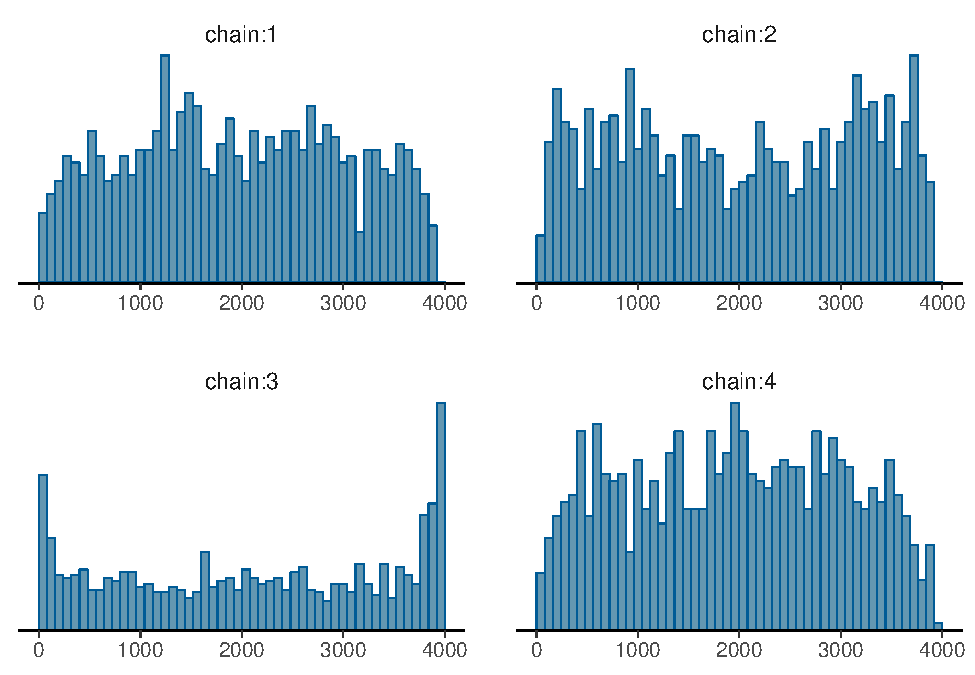
\includegraphics[width=0.6\linewidth]{graphics/hist-fit-nom-td20-1.pdf}
\end{figure}

The rank plot visualisation of \texttt{lp\_\_}, which has an effective
sample size 240, doesn't look so good either.

\begin{figure}[tp]
  \centering
  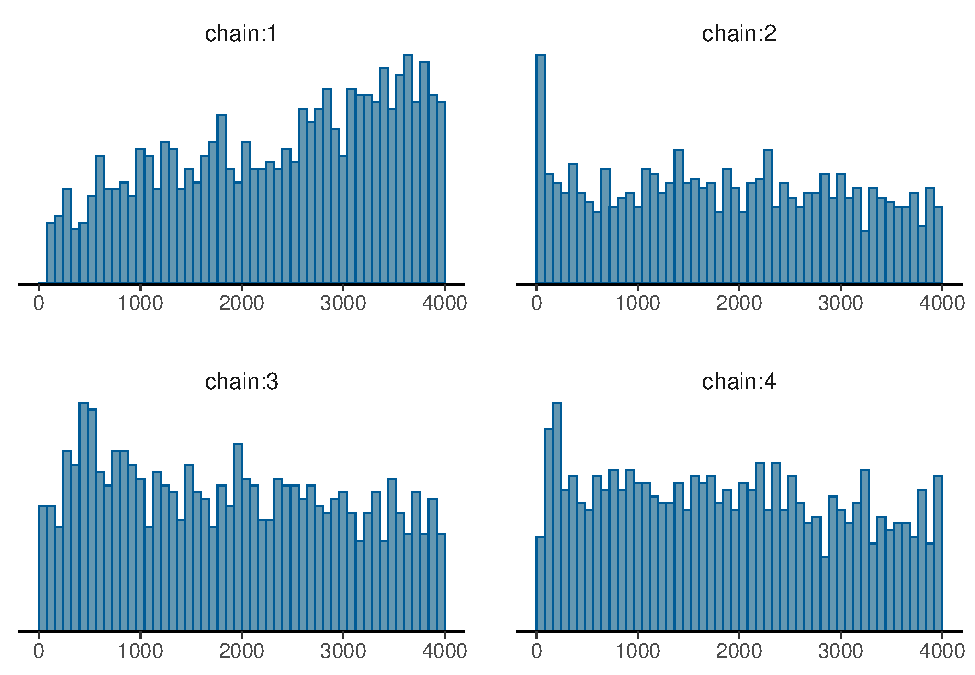
\includegraphics[width=0.6\linewidth]{graphics/hist-fit-nom-td20-lp-1.pdf}
\end{figure}

\hypertarget{default-stan-options-increased-maximum-treedepth-longer-chains}{%
\paragraph{Default Stan options + increased maximum treedepth + longer
chains}\label{default-stan-options-increased-maximum-treedepth-longer-chains}}
\addcontentsline{toc}{paragraph}{Default Stan options + increased
maximum treedepth + longer chains}

Let's try running 8 times longer chains.

Trace plots for the first parameter still look wild with occasional
large values.

\begin{figure}[tp]
  \centering
  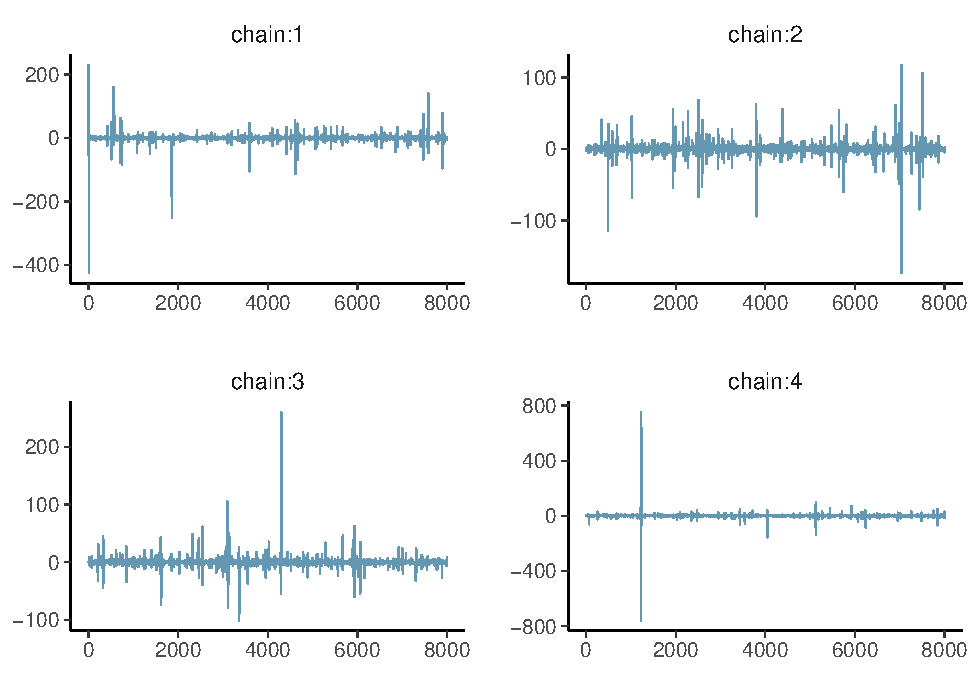
\includegraphics[width=0.6\linewidth]{graphics/trace-fit-nom-td20l-1.pdf}
\end{figure}

Let's check the diagnostics for all \(x\).

\begin{figure}[tp]
  \centering
  \includegraphics[width=0.6\linewidth]{graphics/rhat-fit-nom-td20l-1.pdf}
\end{figure}

All Rhats are below \(1.01\). The classic split-Rhat has more variation
than the rank normalized Rhat (note that the former is not well defined
in this case).

\begin{figure}[tp]
  \centering
  \includegraphics[width=0.6\linewidth]{graphics/ess-fit-nom-td20l-1.pdf}
\end{figure}

Most classic ESS's are close to zero. Running longer chains just made
most classic ESS's even smaller.

The smallest bulk-ESS are around 5000, which is not that bad. The
smallest median-ESS's are larger than 25000, that is we are able to
estimate the median efficiently. However, the smallest tail-ESS is 919
indicating problems for estimating the scale of the posterior.

\textbf{Result:} The rank normalized effective sample size is more
stable than classic effective sample size even for very long chains.

\textbf{Result:} It is useful to look at both bulk- and tail-ESS.

We also check \texttt{lp\_\_}. Although increasing the number of
iterations improved bulk-ESS of the \(x\), the relative efficiency for
\texttt{lp\_\_} didn't change.

\begin{verbatim}
lp__: Bulk-ESS = 1289
\end{verbatim}

\begin{verbatim}
lp__: Tail-ESS = 1887
\end{verbatim}

We examine the sampling efficiency in different parts of the posterior
by computing the effective sample size for small interval probability
estimates.

\begin{figure}[tp]
  \centering
  \includegraphics[width=0.6\linewidth]{graphics/local-ess-fit-nom-td20l-1.pdf}
\end{figure}

Increasing the chain length did not seem to change the relative
efficiency. With more draws from the longer chains we can use a finer
resolution for the local efficiency estimates.

\begin{figure}[tp]
  \centering
  \includegraphics[width=0.6\linewidth]{graphics/local-ess-fit-nom-td20l-finer-1.pdf}
\end{figure}

The sampling efficiency far in the tails is worryingly low. This was
more difficult to see previously with less draws from the tails. We see
similar problems in the plot of effective sample size for quantiles.

\begin{figure}[tp]
  \centering
  \includegraphics[width=0.6\linewidth]{graphics/quantile-ess-fit-nom-td20l-finer-1.pdf}
\end{figure}

Let's look at the rank plot visualisation of x{[}39{]}, which has the
smallest tail-ESS NaN among the \(x\).

\begin{figure}[tp]
  \centering
  \includegraphics[width=0.6\linewidth]{graphics/hist-fit-nom-td20l-1.pdf}
\end{figure}

Increasing the number of iterations couldn't remove the mixing problems
at the tails. The mixing problem is inherent to the nominal
parameterization of Cauchy distribution.

\hypertarget{first-alternative-parameterization-of-the-cauchy-distribution}{%
\subsubsection*{First alternative parameterization of the Cauchy
distribution}\label{first-alternative-parameterization-of-the-cauchy-distribution}}
\addcontentsline{toc}{subsubsection}{First alternative parameterization
of the Cauchy distribution}

Next, we examine an alternative parameterization and consider the Cauchy
distribution as a scale mixture of Gaussian distributions. The model has
two parameters and the Cauchy distributed \(x\) can be computed from
those. In addition to improved sampling performance, the example
illustrates that focusing on diagnostics matters.

\begin{verbatim}
parameters {
  vector[50] x_a;
  vector<lower=0>[50] x_b;
}

transformed parameters {
  vector[50] x = x_a ./ sqrt(x_b);
}

model {
  x_a ~ normal(0, 1);
  x_b ~ gamma(0.5, 0.5);
}

generated quantities {
  real I = fabs(x[1]) < 1 ? 1 : 0;
}
\end{verbatim}

We run the alternative model:

There are no warnings and the sampling is much faster.

\begin{figure}[tp]
  \centering
  \includegraphics[width=0.6\linewidth]{graphics/rhat-fit-alt1-1.pdf}
\end{figure}

All Rhats are below \(1.01\). Classic split-Rhats also look good even
though they are not well defined for the Cauchy distribution.

\begin{figure}[tp]
  \centering
  \includegraphics[width=0.6\linewidth]{graphics/ess-fit-alt1-1.pdf}
\end{figure}

\textbf{Result:} Rank normalized ESS's have less variation than classic
one which is not well defined for Cauchy.

We check \texttt{lp\_\_}:

\begin{verbatim}
lp__: Bulk-ESS = 1310
\end{verbatim}

\begin{verbatim}
lp__: Tail-ESS = 1928
\end{verbatim}

The relative efficiencies for \texttt{lp\_\_} are also much better than
with the nominal parameterization.

We examine the sampling efficiency in different parts of the posterior
by computing the effective sample size for small interval probability
estimates.

\begin{figure}[tp]
  \centering
  \includegraphics[width=0.6\linewidth]{graphics/local-ess-fit-alt1-2-1.pdf}
\end{figure}

The effective sample size is good in all parts of the posterior. We also
examine the effective sample size of different quantile estimates.

\begin{figure}[tp]
  \centering
  \includegraphics[width=0.6\linewidth]{graphics/quantile-ess-fit-alt1-2-1.pdf}
\end{figure}

We compare the mean relative efficiencies of the underlying parameters
in the new parameterization and the actual \(x\) we are interested in.

\begin{verbatim}
Mean Bulk-ESS for x = 3629.24
\end{verbatim}

\begin{verbatim}
Mean Tail-ESS for x = 2265.22
\end{verbatim}

\begin{verbatim}
Mean Bulk-ESS for x_a = 3956.06
\end{verbatim}

\begin{verbatim}
Mean Bulk-ESS for x_b = 2761.22
\end{verbatim}

\textbf{Result:} We see that the effective sample size of the
interesting \(x\) can be different from the effective sample size of the
parameters \(x_a\) and \(x_b\) that we used to compute it.

The rank plot visualisation of x{[}40{]}, which has the smallest
tail-ESS of 1823 among the \(x\) looks better than for the nominal
parameterization.

\begin{figure}[tp]
  \centering
  \includegraphics[width=0.6\linewidth]{graphics/hist-fit-alt1-2-1.pdf}
\end{figure}

Similarly, the rank plot visualisation of \texttt{lp\_\_}, which has a
relative efficiency of -81.34, 0.23, 8.08, -95.19, -80.99, -68.66, 1288,
0.32, 1303, 1296, 1310, 0.33, 1, 1, 1, 1, 1, 2366, 0.59, 1928, 0.48,
1708, 0.43, 2912, 0.73 looks better than for the nominal
parameterization.

\begin{figure}[tp]
  \centering
  \includegraphics[width=0.6\linewidth]{graphics/hist-fit-alt1-lp-1.pdf}
\end{figure}

\hypertarget{another-alternative-parameterization-of-the-cauchy-distribution}{%
\subsubsection*{Another alternative parameterization of the Cauchy
distribution}\label{another-alternative-parameterization-of-the-cauchy-distribution}}
\addcontentsline{toc}{subsubsection}{Another alternative
parameterization of the Cauchy distribution}

Another alternative parameterization is obtained by a univariate
transformation as shown in the following code (see also the 3rd
alternative in Michael Betancourt's case study).

\begin{verbatim}
parameters {
  vector<lower=0, upper=1>[50] x_tilde;
}

transformed parameters {
vector[50] x = tan(pi() * (x_tilde - 0.5));
}

model {
  // Implicit uniform prior on x_tilde
}

generated quantities {
  real I = fabs(x[1]) < 1 ? 1 : 0;
}
\end{verbatim}

We run the alternative model:

There are no warnings, and the sampling is much faster than for the
nominal model.

\begin{figure}[tp]
  \centering
  \includegraphics[width=0.6\linewidth]{graphics/rhat-fit-alt3-1.pdf}
\end{figure}

All Rhats except some folded Rhats are below 1.01. Classic split-Rhat's
look also good even though it is not well defined for the Cauchy
distribution.

\begin{figure}[tp]
  \centering
  \includegraphics[width=0.6\linewidth]{graphics/ess-fit-alt3-1.pdf}
\end{figure}

\textbf{Result:} Rank normalized relative efficiencies have less
variation than classic ones. Bulk-ESS and median-ESS are slightly larger
than 1, which is possible for antithetic Markov chains which have
negative correlation for odd lags.

We also take a closer look at the \texttt{lp\_\_} value:

\begin{verbatim}
lp__: Bulk-ESS = 1494
\end{verbatim}

\begin{verbatim}
lp__: Tail-ESS = 1884
\end{verbatim}

The effective sample size for these are also much better than with the
nominal parameterization.

We examine the sampling efficiency in different parts of the posterior
by computing the effective sample size for small interval probability
estimates.

\begin{figure}[tp]
  \centering
  \includegraphics[width=0.6\linewidth]{graphics/local-ess-fit-alt3-1.pdf}
\end{figure}

We examine also the sampling efficiency of different quantile estimates.

\begin{figure}[tp]
  \centering
  \includegraphics[width=0.6\linewidth]{graphics/quantile-ess-fit-alt3-1.pdf}
\end{figure}

The effective sample size in tails is worse than for the first
alternative parameterization, although it's still better than for the
nominal parameterization.

We compare the mean effective sample size of the underlying parameter in
the new parameterization and the actually Cauchy distributed \(x\) we
are interested in.

\begin{verbatim}
Mean bulk-seff for x = 4702.98
\end{verbatim}

\begin{verbatim}
Mean tail-seff for x = 1602.7
\end{verbatim}

\begin{verbatim}
Mean bulk-seff for x_tilde = 4702.98
\end{verbatim}

\begin{verbatim}
Mean tail-seff for x_tilde = 1612.14
\end{verbatim}

The Rank plot visualisation of x{[}5{]}, which has the smallest tail-ESS
of 1891 among the \(x\) reveals shows good efficiency, similar to the
results for \texttt{lp\_\_}.

\begin{figure}[tp]
  \centering
  \includegraphics[width=0.6\linewidth]{graphics/hist-fit-alt3-1.pdf}
\end{figure}

\begin{figure}[tp]
  \centering
  \includegraphics[width=0.6\linewidth]{graphics/hist-fit-alt3-lp-1.pdf}
\end{figure}

\hypertarget{half-cauchy-distribution-with-nominal-parameterization}{%
\subsubsection*{Half-Cauchy distribution with nominal
parameterization}\label{half-cauchy-distribution-with-nominal-parameterization}}
\addcontentsline{toc}{subsubsection}{Half-Cauchy distribution with
nominal parameterization}

Half-Cauchy priors are common and, for example, in Stan usually set
using the nominal parameterization. However, when the constraint
\texttt{\textless{}lower=0\textgreater{}} is used, Stan does the
sampling automatically in the unconstrained \texttt{log(x)} space, which
changes the geometry crucially.

\begin{verbatim}
parameters {
  vector<lower=0>[50] x;
}

model {
  x ~ cauchy(0, 1);
}

generated quantities {
  real I = fabs(x[1]) < 1 ? 1 : 0;
}
\end{verbatim}

We run the half-Cauchy model with nominal parameterization (and positive
constraint).

There are no warnings and the sampling is much faster than for the full
Cauchy distribution with nominal parameterization.

\begin{figure}[tp]
  \centering
  \includegraphics[width=0.6\linewidth]{graphics/rhat-fit-half-nom-1.pdf}
\end{figure}

All Rhats are below \(1.01\). Classic split-Rhats also look good even
though they are not well defined for the half-Cauchy distribution.

\begin{figure}[tp]
  \centering
  \includegraphics[width=0.6\linewidth]{graphics/ess-fit-half-nom-1.pdf}
\end{figure}

\textbf{Result:} Rank normalized effective sample size have less
variation than classic ones. Some Bulk-ESS and median-ESS are larger
than 1, which is possible for antithetic Markov chains which have
negative correlation for odd lags.

Due to the \texttt{\textless{}lower=0\textgreater{}} constraint, the
sampling was made in the \texttt{log(x)} space, and we can also check
the performance in that space.

\begin{figure}[tp]
  \centering
  \includegraphics[width=0.6\linewidth]{graphics/ess-fit-half-nom-2-1.pdf}
\end{figure}

\(\log(x)\) is quite close to Gaussian, and thus classic effective
sample size is also close to rank normalized ESS which is exactly the
same as for the original \(x\) as rank normalization is invariant to
bijective transformations.

\textbf{Result:} The rank normalized effective sample size is close to
the classic effective sample size for transformations which make the
distribution close to Gaussian.

We examine the sampling efficiency in different parts of the posterior
by computing the effective sample size for small interval probability
estimates.

\begin{figure}[tp]
  \centering
  \includegraphics[width=0.6\linewidth]{graphics/local-ess-fit-half-nom-1.pdf}
\end{figure}

The effective sample size is good overall, with only a small dip in
tails. We can also examine the effective sample size of different
quantile estimates.

\begin{figure}[tp]
  \centering
  \includegraphics[width=0.6\linewidth]{graphics/quantile-ess-fit-half-nom-1.pdf}
\end{figure}

The rank plot visualisation of x{[}32{]}, which has the smallest
tail-ESS of 1742 among \(x\), looks good.

\begin{figure}[tp]
  \centering
  \includegraphics[width=0.6\linewidth]{graphics/hist-fit-half-nom-1.pdf}
\end{figure}

The rank plot visualisation of \texttt{lp\_\_} reveals some small
differences in the scales, but it's difficult to know whether this small
variation from uniform is relevant.

\begin{figure}[tp]
  \centering
  \includegraphics[width=0.6\linewidth]{graphics/hist-fit-half-nom-lp-1.pdf}
\end{figure}

\hypertarget{alternative-parameterization-of-the-half-cauchy-distribution}{%
\subsubsection*{Alternative parameterization of the half-Cauchy
distribution}\label{alternative-parameterization-of-the-half-cauchy-distribution}}
\addcontentsline{toc}{subsubsection}{Alternative parameterization of the
half-Cauchy distribution}

\begin{verbatim}
parameters {
  vector<lower=0>[50] x_a;
  vector<lower=0>[50] x_b;
}

transformed parameters {
  vector[50] x = x_a .* sqrt(x_b);
}

model {
  x_a ~ normal(0, 1);
  x_b ~ inv_gamma(0.5, 0.5);
}

generated quantities {
  real I = fabs(x[1]) < 1 ? 1 : 0;
}
\end{verbatim}

Run half-Cauchy with alternative parameterization

There are no warnings and the sampling is as fast for the half-Cauchy
nominal model.

\begin{figure}[tp]
  \centering
  \includegraphics[width=0.6\linewidth]{graphics/rhat-fit-half-reparam-1.pdf}
\end{figure}

\begin{figure}[tp]
  \centering
  \includegraphics[width=0.6\linewidth]{graphics/ess-fit-half-reparam-1.pdf}
\end{figure}

\textbf{Result:} The Rank normalized relative efficiencies have less
variation than classic ones which is not well defined for the Cauchy
distribution. Based on bulk-ESS and median-ESS, the efficiency for
central quantities is much lower, but based on tail-ESS and MAD-ESS, the
efficiency in the tails is slightly better than for the half-Cauchy
distribution with nominal parameterization. We also see that a
parameterization which is good for the full Cauchy distribution is not
necessarily good for the half-Cauchy distribution as the
\texttt{\textless{}lower=0\textgreater{}} constraint additionally
changes the parameterization.

We also check the \texttt{lp\_\_} values:

\begin{verbatim}
lp__: Bulk-ESS = 977
\end{verbatim}

\begin{verbatim}
lp__: Tail-ESS = 1750
\end{verbatim}

We examine the sampling efficiency in different parts of the posterior
by computing the effective sample size for small interval probability
estimates.

\begin{figure}[tp]
  \centering
  \includegraphics[width=0.6\linewidth]{graphics/local-ess-fit-half-reparam-1.pdf}
\end{figure}

We also examine the effective sample size for different quantile
estimates.

\begin{figure}[tp]
  \centering
  \includegraphics[width=0.6\linewidth]{graphics/quantile-ess-fit-half-reparam-1.pdf}
\end{figure}

The effective sample size near zero is much worse than for the
half-Cauchy distribution with nominal parameterization.

The Rank plot visualisation of x{[}20{]}, which has the smallest
tail-ESS of NaN among the \(x\), reveals deviations from uniformity,
which is expected with lower effective sample size.

\begin{figure}[tp]
  \centering
  \includegraphics[width=0.6\linewidth]{graphics/hist-fit-half-reparam-1.pdf}
\end{figure}

A similar result is obtained when looking at the rank plots of
\texttt{lp\_\_}.

\begin{figure}[tp]
  \centering
  \includegraphics[width=0.6\linewidth]{graphics/hist-fit-half-reparam-lp-1.pdf}
\end{figure}

\hypertarget{the-cauchy-distribution-with-jags}{%
\subsubsection*{The Cauchy distribution with
Jags}\label{the-cauchy-distribution-with-jags}}
\addcontentsline{toc}{subsubsection}{The Cauchy distribution with Jags}

So far, we have run all models in Stan, but we want to also investigate
whether similar problems arise with probabilistic programming languages
that use other samplers than variants of Hamiltonian Monte-Carlo. Thus,
we will fit the eight schools models also with Jags, which uses a
dialect of the BUGS language to specify models. Jags uses a clever mix
of Gibbs and Metropolis-Hastings sampling. This kind of sampling does
not scale well to high dimensional posteriors of strongly interdependent
parameters, but for the relatively simple models discussed in this case
study it should work just fine.

The Jags code for the nominal parameteriztion of the cauchy distribution
looks as follows:

\begin{verbatim}
model {
  for (i in 1:50) {
    x[i] ~ dt(0, 1, 1)
  }
}
\end{verbatim}

First, we initialize the Jags model for reusage later.

\begin{verbatim}
Compiling model graph
   Resolving undeclared variables
   Allocating nodes
Graph information:
   Observed stochastic nodes: 0
   Unobserved stochastic nodes: 50
   Total graph size: 52

Initializing model
\end{verbatim}

Next, we sample 1000 iterations for each of the 4 chains for easy
comparison with the corresponding Stan results.

We summarize the model as follows:

\begin{verbatim}
Inference for the input samples (4 chains: each with iter = 1000; warmup = 0):

         Q5   Q50  Q95   Mean    SD  Rhat Bulk_ESS Tail_ESS
x[1]  -6.16 -0.02 5.78  -3.03 297.0     1     3933     4085
x[2]  -6.73  0.00 6.07  -1.13  57.9     1     4091     3930
x[3]  -6.66  0.01 6.70  -1.23  57.4     1     4026     3826
x[4]  -5.73  0.02 6.51  -0.18  26.2     1     3971     3930
x[5]  -5.72 -0.02 6.20   1.60 119.0     1     4023     3766
x[6]  -6.80 -0.01 5.86   4.80 258.0     1     4037     3925
x[7]  -5.73  0.02 5.85  -0.88  43.8     1     3871     3905
x[8]  -6.19  0.00 6.62   0.21 144.0     1     4103     3753
x[9]  -6.36  0.00 6.63   0.01  28.0     1     4001     4012
x[10] -5.94  0.01 6.99  -0.34  98.4     1     4237     3914
x[11] -6.94 -0.01 6.32  -0.56  25.0     1     3917     3894
x[12] -5.47 -0.01 6.16   0.62  27.7     1     3780     3846
x[13] -6.88 -0.07 6.05  -1.24  91.1     1     3424     3719
x[14] -6.53 -0.03 6.39   2.22 163.0     1     4011     3801
x[15] -6.61 -0.01 6.78   0.11  35.4     1     3628     3685
x[16] -6.46  0.00 5.72 -12.40 521.0     1     4050     3996
x[17] -5.81  0.00 6.42   0.13  37.5     1     4081     3917
x[18] -6.16  0.01 6.35  -8.24 342.0     1     4142     3958
x[19] -6.16  0.00 6.38  -0.24  70.4     1     3879     3785
x[20] -6.59  0.02 6.33   5.38 278.0     1     3864     3888
x[21] -6.46  0.00 5.95   0.91  37.9     1     3820     3598
x[22] -6.33  0.01 6.28  -7.71 518.0     1     3906     3773
x[23] -6.27  0.00 6.82  -3.28 217.0     1     4128     4015
x[24] -7.49 -0.04 5.80   2.30 191.0     1     3993     4103
x[25] -6.19  0.00 5.48   0.36  61.3     1     4163     3852
x[26] -6.12 -0.07 6.31  -2.66 281.0     1     3132     3734
x[27] -6.47  0.02 6.32   1.17  65.6     1     3985     3867
x[28] -6.28  0.02 6.77   3.67 109.0     1     3961     3973
x[29] -5.88 -0.01 6.08  -2.32  68.4     1     3983     3908
x[30] -6.44  0.01 7.10   1.35  55.3     1     4075     3941
x[31] -6.08  0.02 6.21  -0.63  34.1     1     4078     3687
x[32] -5.36 -0.02 6.46  -2.29  73.4     1     3815     3891
x[33] -5.90  0.00 5.84  -0.24  17.7     1     4001     3412
x[34] -6.24 -0.03 6.42  -1.51 132.0     1     3968     3865
x[35] -6.18  0.01 6.41   1.18  49.7     1     3810     3931
x[36] -7.02 -0.01 5.90   6.74 484.0     1     3953     3770
x[37] -6.65 -0.02 6.13   0.14  33.9     1     4048     4101
x[38] -5.83  0.01 6.22   1.97 114.0     1     4172     3840
x[39] -6.28  0.01 6.19   0.15  82.9     1     3933     3929
x[40] -6.31 -0.01 6.57   1.04  97.9     1     4218     3891
x[41] -5.74  0.00 6.57   0.71  54.1     1     3669     3699
x[42] -5.49  0.02 5.59  -0.66  58.2     1     4068     3852
x[43] -6.79 -0.04 6.45  -0.02 109.0     1     3777     3949
x[44] -5.93  0.02 6.17  -0.16  32.9     1     3649     3857
x[45] -6.64  0.00 6.47  -0.33  49.4     1     3919     3869
x[46] -5.41  0.02 6.86   3.27 145.0     1     4069     4013
x[47] -6.27  0.00 5.96  -0.68  22.6     1     3962     4013
x[48] -6.64 -0.02 5.79  -2.35  71.5     1     4015     4016
x[49] -6.71  0.01 6.10   5.69 562.0     1     3886     3809
x[50] -7.00  0.00 6.21   8.79 614.0     1     3830     3884

For each parameter, Bulk_ESS and Tail_ESS are crude measures of 
effective sample size for bulk and tail quantities respectively (good values is 
ESS > 400), and Rhat is the potential scale reduction factor on rank normalized
split chains (at convergence, Rhat = 1).
\end{verbatim}

The overall results look very promising with Rhats = 1 and ESS values
close to the total number of draws of 4000. We take a detailed look at
x{[}26{]}, which has the smallest bulk-ESS of 3132.

We examine the sampling efficiency in different parts of the posterior
by computing the efficiency estimates for small interval probability
estimates.

\begin{figure}[tp]
  \centering
  \includegraphics[width=0.6\linewidth]{graphics/local-ess-jags-nom-1.pdf}
\end{figure}

The efficiency estimate is good in all parts of the posterior. Further,
we examine the sampling efficiency of different quantile estimates.

\begin{figure}[tp]
  \centering
  \includegraphics[width=0.6\linewidth]{graphics/quantile-ess-jags-nom-1.pdf}
\end{figure}

Rank plots also look rather similar across chains.

\begin{figure}[tp]
  \centering
  \includegraphics[width=0.6\linewidth]{graphics/hist-jags-nom-1.pdf}
\end{figure}

\textbf{Result:} Jags seems to be able to sample from the nominal
parameterization of the Cauchy distribution just fine.

\hypertarget{AppendixF}{%
\subsection*{Appendix F: Hierarchical model: Eight
Schools}\label{AppendixF}}
\addcontentsline{toc}{subsection}{Appendix F: Hierarchical model: Eight
Schools}

We continue with our discussion about hierarchical models on the Eight
Schools data, which we started in
\protect\hyperlink{eightschools}{Section Eight Schools}. We also analyse
the performance of different variants of the diagnostics.

\hypertarget{a-centered-eight-schools-model-1}{%
\subsubsection*{A Centered Eight Schools
model}\label{a-centered-eight-schools-model-1}}
\addcontentsline{toc}{subsubsection}{A Centered Eight Schools model}

\begin{verbatim}
data {
  int<lower=0> J;
  real y[J];
  real<lower=0> sigma[J];
}

parameters {
  real mu;
  real<lower=0> tau;
  real theta[J];
}

model {
  mu ~ normal(0, 5);
  tau ~ cauchy(0, 5);
  theta ~ normal(mu, tau);
  y ~ normal(theta, sigma);
}
\end{verbatim}

In the main text, we observed that the centered parameterization of this
hierarchical model did not work well with the default MCMC options of
Stan plus increased \texttt{adapt\_delta}, and so we directly try to fit
the model with longer chains.

\hypertarget{centered-parameterization-with-longer-chains}{%
\paragraph{Centered parameterization with longer
chains}\label{centered-parameterization-with-longer-chains}}
\addcontentsline{toc}{paragraph}{Centered parameterization with longer
chains}

Low efficiency can be sometimes compensated with longer chains. Let's
check 10 times longer chain.

\begin{verbatim}
Inference for the input samples (4 chains: each with iter = 20000; warmup = 10000):

             Q5    Q50   Q95   Mean   SD  Rhat Bulk_ESS Tail_ESS
mu        -0.99   4.84 10.30   4.88 3.57  1.05       71      189
tau        0.33   2.81 10.00   3.67 3.31  1.08       45       17
theta[1]  -1.36   6.43 16.30   6.76 5.64  1.01      407     9491
theta[2]  -2.48   5.47 12.60   5.42 4.80  1.02      153     9429
theta[3]  -4.92   4.66 11.50   4.41 5.43  1.03      117    10374
theta[4]  -2.89   5.34 12.40   5.23 4.97  1.03      140     9670
theta[5]  -4.48   4.32 10.70   4.09 4.94  1.04       89     4758
theta[6]  -4.15   4.70 11.30   4.49 5.08  1.03      118    11277
theta[7]  -0.88   6.60 15.50   6.83 5.11  1.01      449    11102
theta[8]  -3.46   5.41 13.30   5.34 5.49  1.02      172    10408
lp__     -24.90 -14.80  0.22 -13.80 7.59  1.07       50       86

For each parameter, Bulk_ESS and Tail_ESS are crude measures of 
effective sample size for bulk and tail quantities respectively (good values is 
ESS > 400), and Rhat is the potential scale reduction factor on rank normalized
split chains (at convergence, Rhat = 1).
\end{verbatim}

\begin{verbatim}
Inference for the input samples (4 chains: each with iter = 20000; warmup = 10000):

           mean se_mean   sd     Q5    Q50   Q95 seff reff sseff zseff
mu         4.88    0.49 3.57  -0.99   4.84 10.30   53 0.00    71    54
tau        3.67    0.30 3.31   0.33   2.81 10.00  123 0.00   173    35
theta[1]   6.76    0.22 5.64  -1.36   6.43 16.30  666 0.02  1060   281
theta[2]   5.42    0.43 4.80  -2.48   5.47 12.60  124 0.00   169   113
theta[3]   4.41    0.53 5.43  -4.92   4.66 11.50  105 0.00   146    86
theta[4]   5.23    0.46 4.97  -2.89   5.34 12.40  118 0.00   163   105
theta[5]   4.09    0.57 4.94  -4.48   4.32 10.70   76 0.00   102    69
theta[6]   4.49    0.51 5.08  -4.15   4.70 11.30  100 0.00   137    87
theta[7]   6.83    0.23 5.11  -0.88   6.60 15.50  512 0.01   745   309
theta[8]   5.34    0.43 5.49  -3.46   5.41 13.30  162 0.00   231   125
lp__     -13.80    1.32 7.59 -24.90 -14.80  0.22   33 0.00    44    37
         zsseff zsreff  Rhat sRhat zRhat zsRhat zfsRhat zfsseff zfsreff
mu           71   0.00  1.05  1.05  1.05   1.05    1.02     152    0.00
tau          45   0.00  1.02  1.02  1.08   1.08    1.01    1040    0.03
theta[1]    407   0.01  1.01  1.01  1.01   1.01    1.00    3300    0.08
theta[2]    153   0.00  1.02  1.02  1.02   1.02    1.00    1820    0.05
theta[3]    117   0.00  1.03  1.02  1.03   1.03    1.01     736    0.02
theta[4]    140   0.00  1.02  1.02  1.03   1.03    1.01    1470    0.04
theta[5]     89   0.00  1.03  1.03  1.04   1.04    1.01     375    0.01
theta[6]    118   0.00  1.03  1.03  1.03   1.03    1.01     644    0.02
theta[7]    449   0.01  1.01  1.01  1.01   1.01    1.00    2760    0.07
theta[8]    172   0.00  1.02  1.02  1.02   1.02    1.00    2820    0.07
lp__         50   0.00  1.08  1.08  1.07   1.07    1.06      55    0.00
         tailseff tailreff medsseff medsreff madsseff madsreff
mu            189     0.00      174        0      174     0.00
tau            17     0.00      175        0      167     0.00
theta[1]     9490     0.24      177        0      268     0.01
theta[2]     9430     0.24      173        0      177     0.00
theta[3]    10400     0.26      168        0      172     0.00
theta[4]     9670     0.24      167        0      167     0.00
theta[5]     4760     0.12      170        0      178     0.00
theta[6]    11300     0.28      176        0      176     0.00
theta[7]    11100     0.28      179        0      852     0.02
theta[8]    10400     0.26      166        0      191     0.00
lp__           86     0.00      170        0      157     0.00
\end{verbatim}

We still get a whole bunch of divergent transitions so it's clear that
the results can't be trusted even if all other diagnostics were good.
Still, it may be worth looking at additional diagnostics to better
understand what's happening.

Some rank-normalized split-Rhats are still larger than \(1.01\).
Bulk-ESS for $\tau$ and \texttt{lp\_\_} are around 800 which
corresponds to low relative efficiency of \(1\%\), but is above our
recommendation of ESS\textgreater{}400. In this kind of cases, it is
useful to look at the local efficiency estimates, too (and the larger
number of divergences is clear indication of problems, too).

We examine the sampling efficiency in different parts of the posterior
by computing the effective sample size for small intervals for
$\tau$.

\begin{figure}[tp]
  \centering
  \includegraphics[width=0.6\linewidth]{graphics/local-ess-fit-cp2-tau-1.pdf}
\end{figure}

We see that the sampling has difficulties in exploring small
$\tau$ values. As ESS\textless{}400 for small probability
intervals in case of small $\tau$ values, we may suspect that we
may miss substantial amount of posterior mass and get biased estimates.

We also examine the effective sample size of different quantile
estimates.

\begin{figure}[tp]
  \centering
  \includegraphics[width=0.6\linewidth]{graphics/quantile-ess-fit-cp2-tau-1.pdf}
\end{figure}

Several quantile estimates have ESS\textless{}400, which raises a doubt
that there are convergence problems and we may have significant bias.

Let's see how the Bulk-ESS and Tail-ESS changes when we use more and
more draws.

\begin{figure}[tp]
  \centering
  \includegraphics[width=0.6\linewidth]{graphics/change-ess-fit-cp2-tau-1.pdf}
\end{figure}

We see that given recommendation that Bulk-ESS\textgreater{}400 and
Tail-ESS\textgreater{}400, they are not sufficient to detect convergence
problems in this case, even the tail quantile estimates are able to
detect these problems.

The rank plot visualisation of $\tau$ also shows clear sticking
and mixing problems.

\begin{figure}[tp]
  \centering
  \includegraphics[width=0.6\linewidth]{graphics/hist-fit-cp2-tau-1.pdf}
\end{figure}

Similar results are obtained for \texttt{lp\_\_}, which is closely
connected to $\tau$ for this model.

\begin{figure}[tp]
  \centering
  \includegraphics[width=0.6\linewidth]{graphics/hist-fit-cp2-lp-1.pdf}
\end{figure}

We may also examine small interval efficiencies for \texttt{mu}.

\begin{figure}[tp]
  \centering
  \includegraphics[width=0.6\linewidth]{graphics/local-ess-fit-cp2-mu-1.pdf}
\end{figure}

There are gaps of poor efficiency which again indicates problems in the
mixing of the chains. However, these problems do not occur for any
specific range of values of \texttt{mu} as was the case for
$\tau$. This tells us that it's probably not \texttt{mu} with
which the sampler has problems, but more likely $\tau$ or a
related quantity.

As we observed divergences, we shouldn't trust any Monte Carlo standard
error (MCSE) estimates as they are likely biased, as well. However, for
illustration purposes, we compute the MCSE, tail quantiles and
corresponding effective sample sizes for the median of \texttt{mu} and
$\tau$. Comparing to the shorter MCMC run, using 10 times more
draws has not reduced the MCSE to one third as would be expected without
problems in the mixing of the chains.

\begin{verbatim}
  mcse  Q05  Q95   Seff
1 0.37 4.22 5.43 173.52
\end{verbatim}

\begin{verbatim}
  mcse  Q05  Q95   Seff
1 0.27 2.38 3.27 174.86
\end{verbatim}

\hypertarget{centered-parameterization-with-very-long-chains}{%
\paragraph{Centered parameterization with very long
chains}\label{centered-parameterization-with-very-long-chains}}
\addcontentsline{toc}{paragraph}{Centered parameterization with very
long chains}

For further evidence, let's check 100 times longer chains than the
default. This is not something we would recommend doing in practice, as
it is not able to solve any problems with divergences as illustrated
below.

\begin{verbatim}
Inference for the input samples (4 chains: each with iter = 200000; warmup = 100000):

             Q5    Q50   Q95   Mean   SD  Rhat Bulk_ESS Tail_ESS
mu        -1.10   4.37  9.83   4.37 3.33     1    18335    30265
tau        0.47   2.94 10.00   3.80 3.21     1     2200      769
theta[1]  -1.59   5.73 16.40   6.29 5.69     1    23832   110854
theta[2]  -2.53   4.85 12.80   4.94 4.76     1    27789   136002
theta[3]  -5.06   4.09 11.90   3.87 5.36     1    39355   122761
theta[4]  -2.95   4.68 12.60   4.75 4.86     1    32607   138545
theta[5]  -4.55   3.79 10.80   3.55 4.72     1    34479    44492
theta[6]  -4.16   4.16 11.60   4.01 4.91     1    37000    92227
theta[7]  -1.03   5.92 15.60   6.38 5.16     1    20685    58049
theta[8]  -3.49   4.74 13.50   4.85 5.39     1    36212   125498
lp__     -25.00 -15.20 -2.08 -14.60 6.87     1     2541     1074

For each parameter, Bulk_ESS and Tail_ESS are crude measures of 
effective sample size for bulk and tail quantities respectively (good values is 
ESS > 400), and Rhat is the potential scale reduction factor on rank normalized
split chains (at convergence, Rhat = 1).
\end{verbatim}

\begin{verbatim}
Inference for the input samples (4 chains: each with iter = 200000; warmup = 100000):

           mean se_mean   sd     Q5    Q50   Q95  seff reff sseff zseff
mu         4.37    0.02 3.33  -1.10   4.37  9.83 18400 0.05 18400 18400
tau        3.80    0.03 3.21   0.47   2.94 10.00  9360 0.02  9390  2210
theta[1]   6.29    0.03 5.69  -1.59   5.73 16.40 31000 0.08 31100 23800
theta[2]   4.94    0.03 4.76  -2.53   4.85 12.80 32900 0.08 33000 27700
theta[3]   3.87    0.02 5.36  -5.06   4.09 11.90 53600 0.13 53600 39200
theta[4]   4.75    0.02 4.86  -2.95   4.68 12.60 39500 0.10 39700 32500
theta[5]   3.55    0.02 4.72  -4.55   3.79 10.80 41400 0.10 41800 34300
theta[6]   4.01    0.02 4.91  -4.16   4.16 11.60 45900 0.11 46100 36800
theta[7]   6.38    0.03 5.16  -1.03   5.92 15.60 24700 0.06 24700 20700
theta[8]   4.85    0.02 5.39  -3.49   4.74 13.50 50200 0.13 50200 36400
lp__     -14.60    0.14 6.87 -25.00 -15.20 -2.08  2410 0.01  2410  2540
         zsseff zsreff  Rhat sRhat zRhat zsRhat zfsRhat zfsseff zfsreff
mu        18300   0.05     1     1     1      1       1   28800    0.07
tau        2200   0.01     1     1     1      1       1   32900    0.08
theta[1]  23800   0.06     1     1     1      1       1   40600    0.10
theta[2]  27800   0.07     1     1     1      1       1   41800    0.10
theta[3]  39400   0.10     1     1     1      1       1   31400    0.08
theta[4]  32600   0.08     1     1     1      1       1   38700    0.10
theta[5]  34500   0.09     1     1     1      1       1   37200    0.09
theta[6]  37000   0.09     1     1     1      1       1   36600    0.09
theta[7]  20700   0.05     1     1     1      1       1   35100    0.09
theta[8]  36200   0.09     1     1     1      1       1   38900    0.10
lp__       2540   0.01     1     1     1      1       1    2940    0.01
         tailseff tailreff medsseff medsreff madsseff madsreff
mu          30300     0.08    16300     0.04    18300     0.05
tau           769     0.00    10900     0.03    15400     0.04
theta[1]   111000     0.28    15300     0.04    18800     0.05
theta[2]   136000     0.34    15100     0.04    18500     0.05
theta[3]   123000     0.31    16700     0.04    22100     0.06
theta[4]   139000     0.35    16500     0.04    19000     0.05
theta[5]    44500     0.11    16600     0.04    18900     0.05
theta[6]    92200     0.23    16400     0.04    18200     0.05
theta[7]    58000     0.15    14800     0.04    17400     0.04
theta[8]   125000     0.31    15400     0.04    16100     0.04
lp__         1070     0.00    10100     0.03    13800     0.03
\end{verbatim}

Rhat, Bulk-ESS and Tail-ESS are not able to detect problems, although
Tail-ESS for $\tau$ is suspiciously low compared to total number
of draws.

\begin{figure}[tp]
  \centering
  \includegraphics[width=0.6\linewidth]{graphics/local-ess-fit-cp3-tau-1.pdf}
\end{figure}

\begin{figure}[tp]
  \centering
  \includegraphics[width=0.6\linewidth]{graphics/quantile-ess-fit-cp3-tau-1.pdf}
\end{figure}

And the rank plots of $\tau$ also show sticking and mixing
problems for small values of $\tau$.

\begin{figure}[tp]
  \centering
  \includegraphics[width=0.6\linewidth]{graphics/hist-fit-cp3-tau-1.pdf}
\end{figure}

What we do see is an advantage of rank plots over trace plots as even
with 100000 draws per chain, rank plots don't get crowded and the mixing
problems of chains is still easy to see.

With centered parameterization the mean estimate tends to get smaller
with more draws. With 400000 draws using the centered parameterization
the mean estimate is 3.77 (se 0.03). With 40000 draws using the
non-centered parameterization the mean estimate is 3.6 (se 0.02). The
difference is more than 8 sigmas. We are able to see the convergence
problems in the centered parameterization case, if we do look carefully
(or use divergence diagnostic ), but we do see that Rhat, Bulk-ESS,
Tail-ESS and Monte Carlo error estimates for the mean can't be trusted
if other diagnostics indicate convergence problems!

\hypertarget{centered-parameterization-with-very-long-chains-and-thinning}{%
\paragraph{Centered parameterization with very long chains and
thinning}\label{centered-parameterization-with-very-long-chains-and-thinning}}
\addcontentsline{toc}{paragraph}{Centered parameterization with very
long chains and thinning}

When autocorrelation time is high, it has been common to thin the chains
by saving only a small portion of the draws. This will throw away useful
information also for convergence diagnostics. With 400000 iterations per
chain, thinning of 200 and 4 chains, we again end up with 4000
iterations as with the default settings.

We observe several divergent transitions and the estimated Bayesian
fraction of missing information is also low, which indicate convergence
problems and potentially biased estimates.

Unfortunately the thinning makes Rhat and ESS estimates to miss the
problems. The posterior mean is still biased, being more than 3 sigmas
away from the estimate obtained using non-centered parameterization.

\begin{verbatim}
Inference for the input samples (4 chains: each with iter = 400000; warmup = 200000):

             Q5    Q50   Q95   Mean   SD  Rhat Bulk_ESS Tail_ESS
mu        -0.91   4.46  9.73   4.40 3.24     1     3784     3648
tau        0.46   2.89 10.00   3.75 3.16     1     3625     2447
theta[1]  -1.66   5.63 16.20   6.24 5.74     1     4101     3691
theta[2]  -2.17   4.84 12.60   5.04 4.62     1     3950     3946
theta[3]  -4.54   4.16 11.90   3.98 5.21     1     4121     3819
theta[4]  -3.02   4.73 12.40   4.75 4.83     1     4026     4188
theta[5]  -4.38   3.75 10.60   3.55 4.68     1     3790     3839
theta[6]  -3.76   4.30 11.80   4.18 4.86     1     4057     4059
theta[7]  -0.96   5.91 15.40   6.34 5.00     1     4154     3813
theta[8]  -3.54   4.64 13.50   4.78 5.33     1     4040     3968
lp__     -25.10 -15.00 -1.64 -14.40 6.99     1     3689     2616

For each parameter, Bulk_ESS and Tail_ESS are crude measures of 
effective sample size for bulk and tail quantities respectively (good values is 
ESS > 400), and Rhat is the potential scale reduction factor on rank normalized
split chains (at convergence, Rhat = 1).
\end{verbatim}

\begin{verbatim}
Inference for the input samples (4 chains: each with iter = 400000; warmup = 200000):

           mean se_mean   sd     Q5    Q50   Q95 seff reff sseff zseff
mu         4.40    0.05 3.24  -0.91   4.46  9.73 3740 0.93  3780  3740
tau        3.75    0.05 3.16   0.46   2.89 10.00 4010 1.00  4000  3620
theta[1]   6.24    0.09 5.74  -1.66   5.63 16.20 4060 1.02  4070  4100
theta[2]   5.04    0.07 4.62  -2.17   4.84 12.60 3920 0.98  3940  3940
theta[3]   3.98    0.08 5.21  -4.54   4.16 11.90 4100 1.02  4100  4120
theta[4]   4.75    0.08 4.83  -3.02   4.73 12.40 3960 0.99  4010  3970
theta[5]   3.55    0.08 4.68  -4.38   3.75 10.60 3720 0.93  3810  3740
theta[6]   4.18    0.08 4.86  -3.76   4.30 11.80 3940 0.99  4030  4010
theta[7]   6.34    0.08 5.00  -0.96   5.91 15.40 4120 1.03  4130  4140
theta[8]   4.78    0.08 5.33  -3.54   4.64 13.50 3970 0.99  3990  4010
lp__     -14.40    0.12 6.99 -25.10 -15.00 -1.64 3500 0.88  3560  3690
         zsseff zsreff  Rhat sRhat zRhat zsRhat zfsRhat zfsseff zfsreff
mu         3780   0.95     1     1     1      1       1    3660    0.91
tau        3620   0.91     1     1     1      1       1    4100    1.02
theta[1]   4100   1.03     1     1     1      1       1    4200    1.05
theta[2]   3950   0.99     1     1     1      1       1    4050    1.01
theta[3]   4120   1.03     1     1     1      1       1    3810    0.95
theta[4]   4030   1.01     1     1     1      1       1    3920    0.98
theta[5]   3790   0.95     1     1     1      1       1    3580    0.90
theta[6]   4060   1.01     1     1     1      1       1    3880    0.97
theta[7]   4150   1.04     1     1     1      1       1    4060    1.02
theta[8]   4040   1.01     1     1     1      1       1    3750    0.94
lp__       3690   0.92     1     1     1      1       1    3190    0.80
         tailseff tailreff medsseff medsreff madsseff madsreff
mu           3650     0.91     4190     1.05     3800     0.95
tau          2450     0.61     3960     0.99     3820     0.95
theta[1]     3690     0.92     4120     1.03     3900     0.98
theta[2]     3950     0.99     3560     0.89     4060     1.01
theta[3]     3820     0.95     4080     1.02     3810     0.95
theta[4]     4190     1.05     3500     0.87     3880     0.97
theta[5]     3840     0.96     3830     0.96     3840     0.96
theta[6]     4060     1.01     4000     1.00     3820     0.96
theta[7]     3810     0.95     4260     1.06     3870     0.97
theta[8]     3970     0.99     4140     1.03     3830     0.96
lp__         2620     0.65     3840     0.96     3910     0.98
\end{verbatim}

Diagnostic plots for $\tau$ look reasonable as well.

\begin{figure}[tp]
  \centering
  \includegraphics[width=0.6\linewidth]{graphics/local-ess-fit-cp4-tau-1.pdf}
\end{figure}

\begin{figure}[tp]
  \centering
  \includegraphics[width=0.6\linewidth]{graphics/quantile-ess-fit-cp4-tau-1.pdf}
\end{figure}

\begin{figure}[tp]
  \centering
  \includegraphics[width=0.6\linewidth]{graphics/change-ess-fit-cp4-tau-1.pdf}
\end{figure}

However, the rank plots seem still to show the problem.

\begin{figure}[tp]
  \centering
  \includegraphics[width=0.6\linewidth]{graphics/hist-fit-cp4-tau-1.pdf}
\end{figure}

\hypertarget{non-centered-eight-schools-model-1}{%
\subsubsection*{Non-centered Eight Schools
model}\label{non-centered-eight-schools-model-1}}
\addcontentsline{toc}{subsubsection}{Non-centered Eight Schools model}

In the following, we want to expand our understanding of the
non-centered parameterization of the hierarchical model fit to the eight
schools data.

\begin{verbatim}
data {
  int<lower=0> J;
  real y[J];
  real<lower=0> sigma[J];
}

parameters {
  real mu;
  real<lower=0> tau;
  real theta_tilde[J];
}

transformed parameters {
  real theta[J];
  for (j in 1:J)
    theta[j] = mu + tau * theta_tilde[j];
}

model {
  mu ~ normal(0, 5);
  tau ~ cauchy(0, 5);
  theta_tilde ~ normal(0, 1);
  y ~ normal(theta, sigma);
}
\end{verbatim}

\hypertarget{non-centered-parameterization-with-default-mcmc-options}{%
\paragraph{Non-centered parameterization with default MCMC
options}\label{non-centered-parameterization-with-default-mcmc-options}}
\addcontentsline{toc}{paragraph}{Non-centered parameterization with
default MCMC options}

In the main text, we have already seen that the non-centered
parameterization works better than the centered parameterization, at
least when we use an increased \texttt{adapt\_delta} value. Let's see
what happens when using the default MCMC option of Stan.

We observe a few divergent transitions with the default of
\texttt{adapt\_delta=0.8}. Let's analyze the sample.

\begin{verbatim}
Inference for the input samples (4 chains: each with iter = 2000; warmup = 1000):

                   Q5   Q50   Q95  Mean   SD  Rhat Bulk_ESS Tail_ESS
mu              -0.98  4.41  9.52  4.38 3.24     1     4083     2378
tau              0.25  2.77  9.77  3.61 3.16     1     2303     1795
theta_tilde[1]  -1.31  0.35  1.88  0.32 0.97     1     4571     2604
theta_tilde[2]  -1.41  0.14  1.64  0.12 0.92     1     5771     3078
theta_tilde[3]  -1.62 -0.10  1.49 -0.09 0.96     1     4966     3054
theta_tilde[4]  -1.43  0.03  1.51  0.05 0.91     1     5442     2830
theta_tilde[5]  -1.67 -0.17  1.35 -0.16 0.91     1     4273     3005
theta_tilde[6]  -1.64 -0.08  1.48 -0.07 0.95     1     5192     2981
theta_tilde[7]  -1.25  0.39  1.88  0.36 0.97     1     3898     2800
theta_tilde[8]  -1.51  0.07  1.68  0.08 0.97     1     4848     2863
theta[1]        -1.38  5.68 15.80  6.27 5.60     1     3790     2549
theta[2]        -2.29  4.88 12.80  5.03 4.62     1     5002     2920
theta[3]        -4.28  4.08 11.90  3.95 5.24     1     4001     3036
theta[4]        -2.74  4.66 12.10  4.64 4.63     1     4699     3063
theta[5]        -4.13  3.89 10.40  3.63 4.54     1     4310     3184
theta[6]        -4.11  4.19 11.30  3.95 4.88     1     4965     2806
theta[7]        -0.84  5.86 15.20  6.28 4.94     1     4599     3296
theta[8]        -3.24  4.77 13.50  4.91 5.37     1     4461     3288
lp__           -11.10 -6.47 -3.68 -6.81 2.30     1     1711     2385

For each parameter, Bulk_ESS and Tail_ESS are crude measures of 
effective sample size for bulk and tail quantities respectively (good values is 
ESS > 400), and Rhat is the potential scale reduction factor on rank normalized
split chains (at convergence, Rhat = 1).
\end{verbatim}

\begin{verbatim}
Inference for the input samples (4 chains: each with iter = 2000; warmup = 1000):

                mean se_mean   sd     Q5   Q50   Q95 seff reff sseff zseff
mu              4.38    0.05 3.24  -0.98  4.41  9.52 4020 1.01  4040  4070
tau             3.61    0.06 3.16   0.25  2.77  9.77 2680 0.67  2700  2290
theta_tilde[1]  0.32    0.01 0.97  -1.31  0.35  1.88 4530 1.13  4570  4530
theta_tilde[2]  0.12    0.01 0.92  -1.41  0.14  1.64 5740 1.44  5760  5750
theta_tilde[3] -0.09    0.01 0.96  -1.62 -0.10  1.49 4930 1.23  4970  4920
theta_tilde[4]  0.05    0.01 0.91  -1.43  0.03  1.51 5370 1.34  5440  5380
theta_tilde[5] -0.16    0.01 0.91  -1.67 -0.17  1.35 4220 1.06  4270  4230
theta_tilde[6] -0.07    0.01 0.95  -1.64 -0.08  1.48 5180 1.30  5200  5180
theta_tilde[7]  0.36    0.02 0.97  -1.25  0.39  1.88 3880 0.97  3890  3890
theta_tilde[8]  0.08    0.01 0.97  -1.51  0.07  1.68 4840 1.21  4850  4830
theta[1]        6.27    0.09 5.60  -1.38  5.68 15.80 3500 0.88  3530  3770
theta[2]        5.03    0.07 4.62  -2.29  4.88 12.80 4890 1.22  4930  4960
theta[3]        3.95    0.09 5.24  -4.28  4.08 11.90 3800 0.95  3820  3970
theta[4]        4.64    0.07 4.63  -2.74  4.66 12.10 4550 1.14  4580  4680
theta[5]        3.63    0.07 4.54  -4.13  3.89 10.40 4130 1.03  4170  4260
theta[6]        3.95    0.07 4.88  -4.11  4.19 11.30 4730 1.18  4820  4920
theta[7]        6.28    0.07 4.94  -0.84  5.86 15.20 4420 1.10  4420  4520
theta[8]        4.91    0.08 5.37  -3.24  4.77 13.50 4050 1.01  4070  4440
lp__           -6.81    0.06 2.30 -11.10 -6.47 -3.68 1680 0.42  1680  1700
               zsseff zsreff  Rhat sRhat zRhat zsRhat zfsRhat zfsseff
mu               4080   1.02     1     1     1      1       1    1780
tau              2300   0.58     1     1     1      1       1    3130
theta_tilde[1]   4570   1.14     1     1     1      1       1    2140
theta_tilde[2]   5770   1.44     1     1     1      1       1    1980
theta_tilde[3]   4970   1.24     1     1     1      1       1    2140
theta_tilde[4]   5440   1.36     1     1     1      1       1    2010
theta_tilde[5]   4270   1.07     1     1     1      1       1    2260
theta_tilde[6]   5190   1.30     1     1     1      1       1    2080
theta_tilde[7]   3900   0.97     1     1     1      1       1    2260
theta_tilde[8]   4850   1.21     1     1     1      1       1    1900
theta[1]         3790   0.95     1     1     1      1       1    2530
theta[2]         5000   1.25     1     1     1      1       1    2300
theta[3]         4000   1.00     1     1     1      1       1    2550
theta[4]         4700   1.17     1     1     1      1       1    2650
theta[5]         4310   1.08     1     1     1      1       1    2780
theta[6]         4960   1.24     1     1     1      1       1    2670
theta[7]         4600   1.15     1     1     1      1       1    2490
theta[8]         4460   1.12     1     1     1      1       1    2470
lp__             1710   0.43     1     1     1      1       1    2490
               zfsreff tailseff tailreff medsseff medsreff madsseff
mu                0.44     2380     0.59     4240     1.06     2340
tau               0.78     1800     0.45     3150     0.79     3170
theta_tilde[1]    0.54     2600     0.65     4490     1.12     2490
theta_tilde[2]    0.50     3080     0.77     5350     1.34     2410
theta_tilde[3]    0.53     3050     0.76     5400     1.35     2450
theta_tilde[4]    0.50     2830     0.71     4820     1.21     2420
theta_tilde[5]    0.57     3000     0.75     4280     1.07     2690
theta_tilde[6]    0.52     2980     0.75     4760     1.19     2410
theta_tilde[7]    0.56     2800     0.70     3820     0.96     2780
theta_tilde[8]    0.48     2860     0.72     4350     1.09     2000
theta[1]          0.63     2550     0.64     4360     1.09     2790
theta[2]          0.58     2920     0.73     4230     1.06     2540
theta[3]          0.64     3040     0.76     4000     1.00     2970
theta[4]          0.66     3060     0.77     4550     1.14     2860
theta[5]          0.70     3180     0.80     4520     1.13     2690
theta[6]          0.67     2810     0.70     4760     1.19     3150
theta[7]          0.62     3300     0.82     4320     1.08     2910
theta[8]          0.62     3290     0.82     4400     1.10     2640
lp__              0.62     2380     0.60     1990     0.50     2800
               madsreff
mu                 0.59
tau                0.79
theta_tilde[1]     0.62
theta_tilde[2]     0.60
theta_tilde[3]     0.61
theta_tilde[4]     0.60
theta_tilde[5]     0.67
theta_tilde[6]     0.60
theta_tilde[7]     0.70
theta_tilde[8]     0.50
theta[1]           0.70
theta[2]           0.64
theta[3]           0.74
theta[4]           0.71
theta[5]           0.67
theta[6]           0.79
theta[7]           0.73
theta[8]           0.66
lp__               0.70
\end{verbatim}

All Rhats are close to 1, and ESSs are good despite a few divergent
transitions. Small interval and quantile plots of $\tau$ reveal
some sampling problems for small $\tau$ values, but not nearly as
strong as for the centered parameterization.

\begin{figure}[tp]
  \centering
  \includegraphics[width=0.6\linewidth]{graphics/local-ess-fit-ncp-tau-1.pdf}
\end{figure}

\begin{figure}[tp]
  \centering
  \includegraphics[width=0.6\linewidth]{graphics/quantile-ess-fit-ncp-tau-1.pdf}
\end{figure}

Overall, the non-centered parameterization looks good even for the
default settings of \texttt{adapt\_delta}, and increasing it to 0.95
gets rid of the last remaining problems. This stands in sharp contrast
to what we observed for the centered parameterization, where increasing
\texttt{adapt\_delta} didn't help at all. Actually, this is something we
observe quite often: A suboptimal parameterization can cause problems
that are not simply solved by tuning the sampler. Instead, we have to
adjust our model to achieve trustworthy inference.

\hypertarget{eight-schools-with-jags}{%
\subsubsection*{Eight Schools with Jags}\label{eight-schools-with-jags}}
\addcontentsline{toc}{subsubsection}{Eight Schools with Jags}

We will also run the centered and non-centered parameterizations of the
eight schools model with Jags.

\hypertarget{centered-eight-schools-model-1}{%
\paragraph{Centered Eight Schools
Model}\label{centered-eight-schools-model-1}}
\addcontentsline{toc}{paragraph}{Centered Eight Schools Model}

The Jags code for the centered eight schools model looks as follows:

\begin{verbatim}
model {
  for (j in 1:J) {
    sigma_prec[j] <- pow(sigma[j], -2)
    theta[j] ~ dnorm(mu, tau_prec)
    y[j] ~ dnorm(theta[j], sigma_prec[j])
  }
  mu ~ dnorm(0, pow(5, -2))
  tau ~ dt(0, pow(5, -2), 1)T(0, )
  tau_prec <- pow(tau, -2)
}
\end{verbatim}

First, we initialize the Jags model for reusage later.

\begin{verbatim}
Compiling model graph
   Resolving undeclared variables
   Allocating nodes
Graph information:
   Observed stochastic nodes: 8
   Unobserved stochastic nodes: 10
   Total graph size: 40

Initializing model
\end{verbatim}

Next, we sample 1000 iterations for each of the 4 chains for easy
comparison with the corresponding Stan results.

Convergence diagnostics indicate problems in the sampling of \texttt{mu}
and $\tau$, but also to a lesser degree in all other paramters.

\begin{verbatim}
Inference for the input samples (4 chains: each with iter = 1000; warmup = 0):

            Q5  Q50   Q95 Mean   SD  Rhat Bulk_ESS Tail_ESS
mu       -1.00 4.41  9.82 4.42 3.26  1.02      189      447
tau       0.29 2.99  9.96 3.73 3.11  1.08       59       53
theta[1] -1.42 5.71 16.70 6.37 5.57  1.02      280      685
theta[2] -2.33 5.03 13.00 5.03 4.66  1.01      364      956
theta[3] -5.08 4.26 11.90 3.97 5.24  1.01      317      995
theta[4] -2.76 4.92 12.60 4.83 4.82  1.01      374     1001
theta[5] -4.67 3.83 10.70 3.58 4.79  1.01      341      889
theta[6] -4.20 4.29 11.70 4.12 4.83  1.01      377     1052
theta[7] -0.68 5.87 15.40 6.37 4.98  1.02      256      736
theta[8] -3.69 4.97 13.60 4.89 5.35  1.01      415      805

For each parameter, Bulk_ESS and Tail_ESS are crude measures of 
effective sample size for bulk and tail quantities respectively (good values is 
ESS > 400), and Rhat is the potential scale reduction factor on rank normalized
split chains (at convergence, Rhat = 1).
\end{verbatim}

We also see problems in the sampling of $\tau$ using various
diagnostic plots.

\begin{figure}[tp]
  \centering
  \includegraphics[width=0.6\linewidth]{graphics/local-ess-jags-cp-tau-1.pdf}
\end{figure}

\begin{figure}[tp]
  \centering
  \includegraphics[width=0.6\linewidth]{graphics/quantile-ess-jags-cp-tau-1.pdf}
\end{figure}

\begin{figure}[tp]
  \centering
  \includegraphics[width=0.6\linewidth]{graphics/change-ess-jags-cp-tau-1.pdf}
\end{figure}

Let's see what happens if we run 10 times longer chains.

Convergence looks better now, although $\tau$ is still estimated
not very efficiently.

\begin{verbatim}
Inference for the input samples (4 chains: each with iter = 1000; warmup = 0):

            Q5  Q50   Q95 Mean   SD  Rhat Bulk_ESS Tail_ESS
mu       -0.89 4.39 10.20 4.40 3.35  1.06       71      251
tau       0.13 2.37  8.37 3.07 2.69  1.09       36       32
theta[1] -1.34 5.35 14.70 5.79 5.07  1.06       88      924
theta[2] -1.70 4.89 12.30 4.83 4.49  1.04      106      959
theta[3] -3.77 4.10 11.60 3.94 4.89  1.03      148      591
theta[4] -2.34 4.73 12.40 4.68 4.61  1.04      126     1054
theta[5] -3.44 4.01 11.10 3.85 4.46  1.03      153      374
theta[6] -3.37 4.23 11.60 4.07 4.70  1.03      154      619
theta[7] -0.93 5.39 14.60 5.94 4.74  1.07       98      450
theta[8] -2.54 4.68 12.60 4.74 4.82  1.04      130      850

For each parameter, Bulk_ESS and Tail_ESS are crude measures of 
effective sample size for bulk and tail quantities respectively (good values is 
ESS > 400), and Rhat is the potential scale reduction factor on rank normalized
split chains (at convergence, Rhat = 1).
\end{verbatim}

The diagnostic plots of quantiles and small intervals tell a similar
story.

\begin{figure}[tp]
  \centering
  \includegraphics[width=0.6\linewidth]{graphics/local-ess-jags-cp-tau-longer-1.pdf}
\end{figure}

\begin{figure}[tp]
  \centering
  \includegraphics[width=0.6\linewidth]{graphics/quantile-ess-jags-cp-tau-longer-1.pdf}
\end{figure}

Notably, however, the increase in effective sample size of tau is linear
in the total number of draws indicating that convergence for
$\tau$ may be achieved by simply running longer chains.

\begin{figure}[tp]
  \centering
  \includegraphics[width=0.6\linewidth]{graphics/change-ess-jags-cp-tau-longer-1.pdf}
\end{figure}

\textbf{Result:} Similar to Stan, Jags also has convergence problems
with the centered parameterization of the eight schools model.

\hypertarget{non-centered-eight-schools-model-2}{%
\paragraph{Non-Centered Eight Schools
Model}\label{non-centered-eight-schools-model-2}}
\addcontentsline{toc}{paragraph}{Non-Centered Eight Schools Model}

The Jags code for the non-centered eight schools model looks as follows:

\begin{verbatim}
model {
  for (j in 1:J) {
    sigma_prec[j] <- pow(sigma[j], -2)
    theta_tilde[j] ~ dnorm(0, 1)
    theta[j] = mu + tau * theta_tilde[j]
    y[j] ~ dnorm(theta[j], sigma_prec[j])
  }
  mu ~ dnorm(0, pow(5, -2))
  tau ~ dt(0, pow(5, -2), 1)T(0, )
}
\end{verbatim}

First, we initialize the Jags model for reusage later.

\begin{verbatim}
Compiling model graph
   Resolving undeclared variables
   Allocating nodes
Graph information:
   Observed stochastic nodes: 8
   Unobserved stochastic nodes: 10
   Total graph size: 55

Initializing model
\end{verbatim}

Next, we sample 1000 iterations for each of the 4 chains for easy
comparison with the corresponding Stan results.

Convergence diagnostics indicate much better mixing than for the
centered eight school model.

\begin{verbatim}
Inference for the input samples (4 chains: each with iter = 1000; warmup = 0):

            Q5  Q50  Q95 Mean   SD  Rhat Bulk_ESS Tail_ESS
mu       -1.00 4.43 10.1 4.44 3.39     1     2897     3447
tau       0.26 2.74 10.2 3.64 3.28     1     1031      965
theta[1] -1.63 5.63 16.5 6.30 5.76     1     3218     2337
theta[2] -2.60 4.91 12.8 5.00 4.78     1     4015     2912
theta[3] -5.00 4.07 11.9 3.86 5.35     1     3189     2725
theta[4] -2.54 4.78 12.4 4.88 4.79     1     3440     3488
theta[5] -4.44 3.91 10.9 3.64 4.67     1     3480     3560
theta[6] -4.16 4.12 11.4 3.94 4.77     1     3345     2715
theta[7] -1.06 5.95 15.9 6.42 5.16     1     3081     2721
theta[8] -3.43 4.83 13.7 4.92 5.36     1     4112     3115

For each parameter, Bulk_ESS and Tail_ESS are crude measures of 
effective sample size for bulk and tail quantities respectively (good values is 
ESS > 400), and Rhat is the potential scale reduction factor on rank normalized
split chains (at convergence, Rhat = 1).
\end{verbatim}

Specifically, the mixing of $\tau$ looks much better although we
still see some problems in the estimation of larger quantiles.

\begin{figure}[tp]
  \centering
  \includegraphics[width=0.6\linewidth]{graphics/local-ess-jags-ncp-tau-1.pdf}
\end{figure}

\begin{figure}[tp]
  \centering
  \includegraphics[width=0.6\linewidth]{graphics/quantile-ess-jags-ncp-tau-1.pdf}
\end{figure}

Change in effective sample size is roughly linear indicating that some
remaining convergence problems are likely to be solved by running longer
chains.

\begin{figure}[tp]
  \centering
  \includegraphics[width=0.6\linewidth]{graphics/change-ess-jags-ncp-tau-1.pdf}
\end{figure}

\textbf{Result:} Similar to Stan, Jags can sample from the non-centered
parameterization of the eight schools model much better than from the
centered parameterization.

\hypertarget{AppendixG}{%
\subsection*{Appendix G: Dynamic HMC and effective sample
size}\label{AppendixG}}
\addcontentsline{toc}{subsection}{Appendix G: Dynamic HMC and effective
sample size}

We have already seen that the effective sample size of dynamic HMC can
be higher than with independent draws. The next example illustrates
interesting relative efficiency phenomena due to the properties of
dynamic HMC algorithms.

We sample from a simple 16-dimensional standard normal model.

\begin{verbatim}
data {
  int<lower=1> J;
}
parameters {
  vector[J] x;
}
model {
  x ~ normal(0, 1);
}
\end{verbatim}

\begin{verbatim}
Inference for the input samples (4 chains: each with iter = 10000; warmup = 0):

          Q5   Q50   Q95  Mean   SD  Rhat Bulk_ESS Tail_ESS
x[1]   -1.66  0.00  1.65  0.00 1.00     1    98264    28709
x[2]   -1.64 -0.01  1.64  0.00 1.00     1    95812    29664
x[3]   -1.63  0.00  1.62  0.00 0.99     1    98640    28669
x[4]   -1.65  0.00  1.66  0.01 1.01     1    97302    29166
x[5]   -1.64  0.00  1.63  0.00 1.00     1   101542    29930
x[6]   -1.65  0.00  1.65  0.00 1.00     1    96292    28376
x[7]   -1.63  0.01  1.63  0.00 0.99     1    96016    29238
x[8]   -1.65 -0.01  1.65  0.00 1.00     1   100375    29893
x[9]   -1.64  0.01  1.65  0.00 1.00     1   101141    28621
x[10]  -1.62 -0.01  1.63  0.00 0.99     1   103126    29411
x[11]  -1.65  0.01  1.66  0.00 1.00     1    95886    28488
x[12]  -1.62  0.00  1.63  0.01 0.99     1    98433    29228
x[13]  -1.62  0.01  1.65  0.00 0.99     1    98181    27421
x[14]  -1.63  0.00  1.63  0.00 0.99     1    97313    27507
x[15]  -1.63  0.01  1.64  0.01 0.99     1    95223    29139
x[16]  -1.66  0.00  1.65  0.00 1.01     1    99980    29639
lp__  -13.00 -7.66 -3.92 -7.95 2.79     1    14489    19627

For each parameter, Bulk_ESS and Tail_ESS are crude measures of 
effective sample size for bulk and tail quantities respectively (good values is 
ESS > 400), and Rhat is the potential scale reduction factor on rank normalized
split chains (at convergence, Rhat = 1).
\end{verbatim}

\begin{verbatim}
Inference for the input samples (4 chains: each with iter = 10000; warmup = 0):

       mean se_mean   sd     Q5   Q50   Q95   seff reff  sseff  zseff
x[1]   0.00    0.00 1.00  -1.66  0.00  1.65  97800 2.45  98400  97700
x[2]   0.00    0.00 1.00  -1.64 -0.01  1.64  95400 2.39  95700  95500
x[3]   0.00    0.00 0.99  -1.63  0.00  1.62  98400 2.46  98700  98300
x[4]   0.01    0.00 1.01  -1.65  0.00  1.66  96600 2.42  97300  96700
x[5]   0.00    0.00 1.00  -1.64  0.00  1.63 101000 2.53 102000 101000
x[6]   0.00    0.00 1.00  -1.65  0.00  1.65  96000 2.40  96300  96000
x[7]   0.00    0.00 0.99  -1.63  0.01  1.63  95600 2.39  96100  95500
x[8]   0.00    0.00 1.00  -1.65 -0.01  1.65  99900 2.50 100000  99900
x[9]   0.00    0.00 1.00  -1.64  0.01  1.65 101000 2.52 101000 101000
x[10]  0.00    0.00 0.99  -1.62 -0.01  1.63 102000 2.55 103000 102000
x[11]  0.00    0.00 1.00  -1.65  0.01  1.66  95200 2.38  95900  95200
x[12]  0.01    0.00 0.99  -1.62  0.00  1.63  97800 2.45  98400  97900
x[13]  0.00    0.00 0.99  -1.62  0.01  1.65  97700 2.44  98200  97700
x[14]  0.00    0.00 0.99  -1.63  0.00  1.63  96800 2.42  97300  96800
x[15]  0.01    0.00 0.99  -1.63  0.01  1.64  94900 2.37  95200  95000
x[16]  0.00    0.00 1.01  -1.66  0.00  1.65  99500 2.49 100000  99400
lp__  -7.95    0.02 2.79 -13.00 -7.66 -3.92  14900 0.37  14900  14500
      zsseff zsreff  Rhat sRhat zRhat zsRhat zfsRhat zfsseff zfsreff
x[1]   98300   2.46     1     1     1      1       1   16400    0.41
x[2]   95800   2.40     1     1     1      1       1   16500    0.41
x[3]   98600   2.47     1     1     1      1       1   16200    0.40
x[4]   97300   2.43     1     1     1      1       1   16100    0.40
x[5]  102000   2.54     1     1     1      1       1   16800    0.42
x[6]   96300   2.41     1     1     1      1       1   16600    0.41
x[7]   96000   2.40     1     1     1      1       1   17100    0.43
x[8]  100000   2.51     1     1     1      1       1   16400    0.41
x[9]  101000   2.53     1     1     1      1       1   15900    0.40
x[10] 103000   2.58     1     1     1      1       1   16500    0.41
x[11]  95900   2.40     1     1     1      1       1   16000    0.40
x[12]  98400   2.46     1     1     1      1       1   15300    0.38
x[13]  98200   2.45     1     1     1      1       1   15400    0.38
x[14]  97300   2.43     1     1     1      1       1   16500    0.41
x[15]  95200   2.38     1     1     1      1       1   16700    0.42
x[16] 100000   2.50     1     1     1      1       1   16400    0.41
lp__   14500   0.36     1     1     1      1       1   21500    0.54
      tailseff tailreff medsseff medsreff madsseff madsreff
x[1]     28700     0.72    82400     2.06    19200     0.48
x[2]     29700     0.74    75500     1.89    19200     0.48
x[3]     28700     0.72    78600     1.97    18700     0.47
x[4]     29200     0.73    81100     2.03    19100     0.48
x[5]     29900     0.75    80000     2.00    20100     0.50
x[6]     28400     0.71    79000     1.98    19600     0.49
x[7]     29200     0.73    81700     2.04    19500     0.49
x[8]     29900     0.75    79300     1.98    18800     0.47
x[9]     28600     0.72    81100     2.03    18700     0.47
x[10]    29400     0.74    76900     1.92    19200     0.48
x[11]    28500     0.71    79200     1.98    18300     0.46
x[12]    29200     0.73    81800     2.05    18700     0.47
x[13]    27400     0.69    80600     2.02    18200     0.46
x[14]    27500     0.69    77600     1.94    19000     0.48
x[15]    29100     0.73    80400     2.01    19600     0.49
x[16]    29600     0.74    82300     2.06    18800     0.47
lp__     19600     0.49    17100     0.43    23600     0.59
\end{verbatim}

The Bulk-ESS for all \(x\) is larger than 95223. However tail-ESS for
all \(x\) is less than 29930. Further, bulk-ESS for \texttt{lp\_\_} is
only 14489.\\
If we take a look at all the Stan examples in this notebook, we see that
the bulk-ESS for \texttt{lp\_\_} is always below 0.5. This is because
\texttt{lp\_\_} correlates strongly with the total energy in HMC, which
is sampled using a random walk proposal once per iteration. Thus, it's
likely that \texttt{lp\_\_} has some random walk behavior, as well,
leading to autocorrelation and a small relative efficiency. At the same
time, adaptive HMC can create antithetic Markov chains which have
negative auto-correlations at odd lags. This results in a bulk-ESS
greater than S for some parameters.

Let's check the effective sample size in different parts of the
posterior by computing the effective sample size for small interval
estimates for \texttt{x{[}1{]}}.

\begin{figure}[tp]
  \centering
  \includegraphics[width=0.6\linewidth]{graphics/local-ess-fit-n-1.pdf}
\end{figure}

The effective sample size for probability estimate for a small interval
is close to 1 with a slight drop in the tails. This is a good result,
but far from the effective sample size for the bulk, mean, and median
estimates. Let's check the effective sample size for quantiles.

\begin{figure}[tp]
  \centering
  \includegraphics[width=0.6\linewidth]{graphics/quantile-ess-fit-n-1.pdf}
\end{figure}

Central quantile estimates have higher effective sample size than tail
quantile estimates.

The total energy of HMC should affect how far in the tails a chain in
one iteration can go. Fat tails of the target have high energy, and thus
only chains with high total energy can reach there. This will suggest
that the random walk in total energy would cause random walk in the
variance of \(x\). Let's check the second moment of \(x\).

\begin{verbatim}
Inference for the input samples (4 chains: each with iter = 10000; warmup = 0):

      Q5  Q50  Q95 Mean   SD  Rhat Bulk_ESS Tail_ESS
x[1]   0 0.46 3.85 1.01 1.44     1    16443    18225
x[2]   0 0.44 3.80 0.99 1.42     1    16492    19392
x[3]   0 0.45 3.80 0.98 1.39     1    16148    18342
x[4]   0 0.45 3.95 1.01 1.46     1    16070    18288
x[5]   0 0.45 3.86 1.00 1.42     1    16785    18672
x[6]   0 0.45 3.91 1.00 1.42     1    16572    17525
x[7]   0 0.45 3.74 0.99 1.39     1    17097    19120
x[8]   0 0.46 3.80 1.00 1.42     1    16397    18152
x[9]   0 0.45 3.81 1.00 1.41     1    15922    18049
x[10]  0 0.44 3.73 0.98 1.39     1    16461    18098
x[11]  0 0.46 3.85 1.00 1.41     1    16008    19463
x[12]  0 0.45 3.75 0.99 1.41     1    15368    17674
x[13]  0 0.44 3.83 0.98 1.38     1    15371    16755
x[14]  0 0.45 3.75 0.98 1.37     1    16461    17715
x[15]  0 0.45 3.77 0.98 1.38     1    16655    19241
x[16]  0 0.47 3.86 1.01 1.41     1    16400    19741

For each parameter, Bulk_ESS and Tail_ESS are crude measures of 
effective sample size for bulk and tail quantities respectively (good values is 
ESS > 400), and Rhat is the potential scale reduction factor on rank normalized
split chains (at convergence, Rhat = 1).
\end{verbatim}

\begin{verbatim}
Inference for the input samples (4 chains: each with iter = 10000; warmup = 0):

      mean se_mean   sd Q5  Q50  Q95  seff reff sseff zseff zsseff zsreff
x[1]  1.01    0.01 1.44  0 0.46 3.85 14700 0.37 14700 16400  16400   0.41
x[2]  0.99    0.01 1.42  0 0.44 3.80 15500 0.39 15500 16500  16500   0.41
x[3]  0.98    0.01 1.39  0 0.45 3.80 14700 0.37 14700 16100  16100   0.40
x[4]  1.01    0.01 1.46  0 0.45 3.95 14500 0.36 14500 16000  16100   0.40
x[5]  1.00    0.01 1.42  0 0.45 3.86 15000 0.38 15000 16800  16800   0.42
x[6]  1.00    0.01 1.42  0 0.45 3.91 14400 0.36 14400 16500  16600   0.41
x[7]  0.99    0.01 1.39  0 0.45 3.74 15500 0.39 15500 17100  17100   0.43
x[8]  1.00    0.01 1.42  0 0.46 3.80 14800 0.37 14800 16400  16400   0.41
x[9]  1.00    0.01 1.41  0 0.45 3.81 13400 0.34 13500 15900  15900   0.40
x[10] 0.98    0.01 1.39  0 0.44 3.73 14700 0.37 14700 16400  16500   0.41
x[11] 1.00    0.01 1.41  0 0.46 3.85 15100 0.38 15100 16000  16000   0.40
x[12] 0.99    0.01 1.41  0 0.45 3.75 14200 0.36 14200 15300  15400   0.38
x[13] 0.98    0.01 1.38  0 0.44 3.83 13500 0.34 13500 15400  15400   0.38
x[14] 0.98    0.01 1.37  0 0.45 3.75 14500 0.36 14600 16400  16500   0.41
x[15] 0.98    0.01 1.38  0 0.45 3.77 15400 0.39 15400 16700  16700   0.42
x[16] 1.01    0.01 1.41  0 0.47 3.86 15600 0.39 15600 16400  16400   0.41
       Rhat sRhat zRhat zsRhat zfsRhat zfsseff zfsreff tailseff tailreff
x[1]      1     1     1      1       1   18400    0.46    18200     0.46
x[2]      1     1     1      1       1   19700    0.49    19400     0.48
x[3]      1     1     1      1       1   18500    0.46    18300     0.46
x[4]      1     1     1      1       1   19000    0.47    18300     0.46
x[5]      1     1     1      1       1   19500    0.49    18700     0.47
x[6]      1     1     1      1       1   17500    0.44    17500     0.44
x[7]      1     1     1      1       1   19000    0.48    19100     0.48
x[8]      1     1     1      1       1   18900    0.47    18200     0.45
x[9]      1     1     1      1       1   18400    0.46    18000     0.45
x[10]     1     1     1      1       1   18600    0.46    18100     0.45
x[11]     1     1     1      1       1   19500    0.49    19500     0.49
x[12]     1     1     1      1       1   18700    0.47    17700     0.44
x[13]     1     1     1      1       1   18500    0.46    16800     0.42
x[14]     1     1     1      1       1   18800    0.47    17700     0.44
x[15]     1     1     1      1       1   19600    0.49    19200     0.48
x[16]     1     1     1      1       1   20100    0.50    19700     0.49
      medsseff medsreff madsseff madsreff
x[1]     19200     0.48    23300     0.58
x[2]     19300     0.48    24900     0.62
x[3]     18700     0.47    23900     0.60
x[4]     19200     0.48    23900     0.60
x[5]     20100     0.50    25000     0.63
x[6]     19600     0.49    22600     0.57
x[7]     19600     0.49    23300     0.58
x[8]     18800     0.47    24200     0.60
x[9]     18700     0.47    22200     0.55
x[10]    19100     0.48    23900     0.60
x[11]    18400     0.46    24700     0.62
x[12]    18600     0.46    24000     0.60
x[13]    18300     0.46    24100     0.60
x[14]    19100     0.48    23400     0.59
x[15]    19600     0.49    24500     0.61
x[16]    18800     0.47    24400     0.61
\end{verbatim}

The mean of the bulk-ESS for \(x_j^2\) is 16290.62, which is quite close
to the bulk-ESS for \texttt{lp\_\_}. This is not that surprising as the
potential energy in normal model is proportional to
\(\sum_{j=1}^J x_j^2\).

Let's check the effective sample size in different parts of the
posterior by computing the effective sample size for small interval
probability estimates for \texttt{x{[}1{]}\^{}2}.

\begin{figure}[tp]
  \centering
  \includegraphics[width=0.6\linewidth]{graphics/local-ess-fit-n-2-1.pdf}
\end{figure}

The effective sample size is mostly a bit below 1, but for the right
tail of \(x_1^2\) the effective sample size drops. This is likely due to
only some iterations having high enough total energy to obtain draws
from the high energy part of the tail. Let's check the effective sample
size for quantiles.

\begin{figure}[tp]
  \centering
  \includegraphics[width=0.6\linewidth]{graphics/quantile-ess-fit-n-2-1.pdf}
\end{figure}

We can see the correlation between \texttt{lp\_\_} and magnitude of
\texttt{x{[}1{]}} in the following plot.

\begin{figure}[tp]
  \centering
  \includegraphics[width=0.6\linewidth]{graphics/qplot-fit-n-1.pdf}
\end{figure}

Low \texttt{lp\_\_} values corresponds to high energy and more variation
in \texttt{x{[}1{]}}, and high \texttt{lp\_\_} corresponds to low energy
and small variation in \texttt{x{[}1{]}}. Finally \(\sum_{j=1}^J x_j^2\)
is perfectly correlated with \texttt{lp\_\_}.

\begin{figure}[tp]
  \centering
  \includegraphics[width=0.6\linewidth]{graphics/qplot-fit-n-2-1.pdf}
\end{figure}

This shows that even if we get high effective sample size estimates for
central quantities (like mean or median), it is important to look at the
relative efficiency of scale and tail quantities, as well. The effective
sample size of \texttt{lp\_\_} can also indicate problems of sampling in
the tails.

\newpage

\hypertarget{refs}{}

\bibliography{rhat}


\end{document}
